%This file is part of diplom-kovalev
%Copyright (C) 2012 Maxim Kovalev.
%Permission is granted to copy, distribute and/or modify this document
%under the terms of the GNU Free Documentation License, Version 1.3
%or any later version published by the Free Software Foundation;
%with no Invariant Sections, no Front-Cover Texts, and no Back-Cover Texts.
%A copy of the license is included in the section entitled "GNU
%Free Documentation License".

\documentclass[a4paper,14pt]{extreport}
\usepackage[T2A,T1]{fontenc}
\usepackage[utf8]{inputenc}
\usepackage[english,russian]{babel}
\usepackage[unicode]{hyperref}
\hypersetup{colorlinks,
	citecolor=black,
	filecolor=black,
	linkcolor=black,
	urlcolor=black,
	bookmarksopen=true,
	pdftex}
\hfuzz = .6pt % avoid black boxes
\usepackage{amssymb,amsfonts,amsmath,mathtext,cite,enumerate,float} 
\usepackage{graphicx}
\graphicspath{{images/}}
\usepackage[absolute]{textpos}
\usepackage{afterpage}
\usepackage[titletoc]{appendix}
\usepackage{titlesec}
\usepackage{listings}
\usepackage{caption}
\usepackage{subcaption}
\usepackage{cmap}


\makeatletter %	иначе не работают вместе hyperref, appendix и babel
\let\oriAlph\Alph
\let\orialph\alph
\renewcommand{\@resets@pp}{\par
	\@ppsavesec
	\stepcounter{@pps}
	\setcounter{section}{0}%
	\if@chapter@pp
		\setcounter{chapter}{0}%
		\renewcommand\@chapapp{\appendixname}%
		\renewcommand\thechapter{\@Alph\c@chapter}%
	\else
		\setcounter{subsection}{0}%
		\renewcommand\thesection{\@Alph\c@section}%
	\fi
	\if@pphyper
		\if@chapter@pp
			\renewcommand{\theHchapter}{\theH@pps.\oriAlph{chapter}}%
		\else
			\renewcommand{\theHsection}{\theH@pps.\oriAlph{section}}%
		\fi
		\def\Hy@chapapp{appendix}%
	\fi
	\restoreapp
}
\makeatother


\makeatletter
\renewcommand{\@biblabel}[1]{#1.} %Заменяем библиографию с квадратных скобок на точку
\renewcommand\bibname{Литература}
\makeatother

\bibliographystyle{unsrt}

\usepackage{geometry}	%Меняем поля страницы
\geometry{left=2cm}	% левое поле
\geometry{right=1.5cm}	% правое поле
\geometry{top=1cm}	% верхнее поле
\geometry{bottom=2cm}	% нижнее поле

\renewcommand{\theenumi}{\arabic{enumi}}					% Меняем везде перечисления на цифра.цифра
\renewcommand{\labelenumi}{\arabic{enumi}}					% Меняем везде перечисления на цифра.цифра
\renewcommand{\theenumii}{.\arabic{enumii}}					% Меняем везде перечисления на цифра.цифра
\renewcommand{\labelenumii}{\arabic{enumi}.\arabic{enumii}.}			% Меняем везде перечисления на цифра.цифра
\renewcommand{\theenumiii}{.\arabic{enumiii}}					% Меняем везде перечисления на цифра.цифра
\renewcommand{\labelenumiii}{\arabic{enumi}.\arabic{enumii}.\arabic{enumiii}.}	% Меняем везде перечисления на цифра.цифра

\renewcommand{\baselinestretch}{1.25} %полуторный интервал 


\titleformat{\chapter}[hang] 
{\normalfont\huge\bfseries}{\thechapter}{1em}{} 
\titleformat{\section}[hang] 
{\normalfont\large\bfseries}{\thesection}{1em}{} 
\titleformat{\subsection}[hang] 
{\normalfont\normalsize\bfseries}{\thesubsection}{1em}{} 
\titleformat{\subsubsection}[hang] 
{\normalfont\small\bfseries}{\thesubsubsection}{1em}{} 
\setcounter{secnumdepth}{4}
\setcounter{tocdepth}{4}


\begin{document}
%This file is part of diplom-kovalev
%Copyright (C) 2012 Maxim Kovalev.
%Permission is granted to copy, distribute and/or modify this document
%under the terms of the GNU Free Documentation License, Version 1.3
%or any later version published by the Free Software Foundation;
%with no Invariant Sections, no Front-Cover Texts, and no Back-Cover Texts.
%A copy of the license is included in the section entitled "GNU
%Free Documentation License".

\begin{titlepage}
\newpage

\begin{center}
\hrulefill\\
{\smallМИНИСТЕРСТВО ОБРАЗОВАНИЯ И НАУКИ РОССИЙСКОЙ ФЕДЕРАЦИИ\\
МОСКОВСКИЙ ГОСУДАРСТВЕННЫЙ ИНСТИТУТ ЭЛЕКТРОНИКИ И МАТЕМАТИКИ\\*
(ТЕХНИЧЕСКИЙ УНИВЕРСИТЕТ)}\\*
\vspace{1em}
КАФЕДРА ИНФОРМАЦИОННО--КОММУНИКАЦИОННЫЕ ТЕХНОЛОГИИ
\end{center}


\vspace{1em}

\begin{center}
\Large Пояснительная записка \\ к дипломной работе на тему:
\end{center}

\vspace{1em}

\begin{center}
\textsc{\textbf{Разработка системы позиционирования транспорта по сигналам сотовых сетей}}
\end{center}

\vfill

\begin{flushleft}
Студент: \hfill Ковалев М.М.\\
\vspace{3em}
Руководитель проекта: \hfill Столяров Д.О.\\
\vspace{3em}
Допущен к защите: \hfill <<\rule{1em}{0.01pt}>> \rule{5em}{0.01pt} 2012 г.\\
\vspace{2.5em}
Консультанты проекта:\\
Охрана труда: \hfill Михайлов Е.Б.\\
\vspace{2.5em}
Заведующий кафедрой: \hfill Азаров В.Н.\\
\end{flushleft}

\vspace{\fill}

\begin{center}
Москва, 2012г.
\end{center}

\end{titlepage}
	% это титульный лист
%This file is part of diplom-kovalev
%Copyright (C) 2012 Maxim Kovalev.
%Permission is granted to copy, distribute and/or modify this document
%under the terms of the GNU Free Documentation License, Version 1.3
%or any later version published by the Free Software Foundation;
%with no Invariant Sections, no Front-Cover Texts, and no Back-Cover Texts.
%A copy of the license is included in the section entitled "GNU
%Free Documentation License".

%\chapter*{Техническое задание}
\addcontentsline{toc}{chapter}{Техническое задание}
\afterpage{%
	\newpage%
	\thispagestyle{empty}%
	\begin{textblock*}{297mm}(0mm,0mm)%
		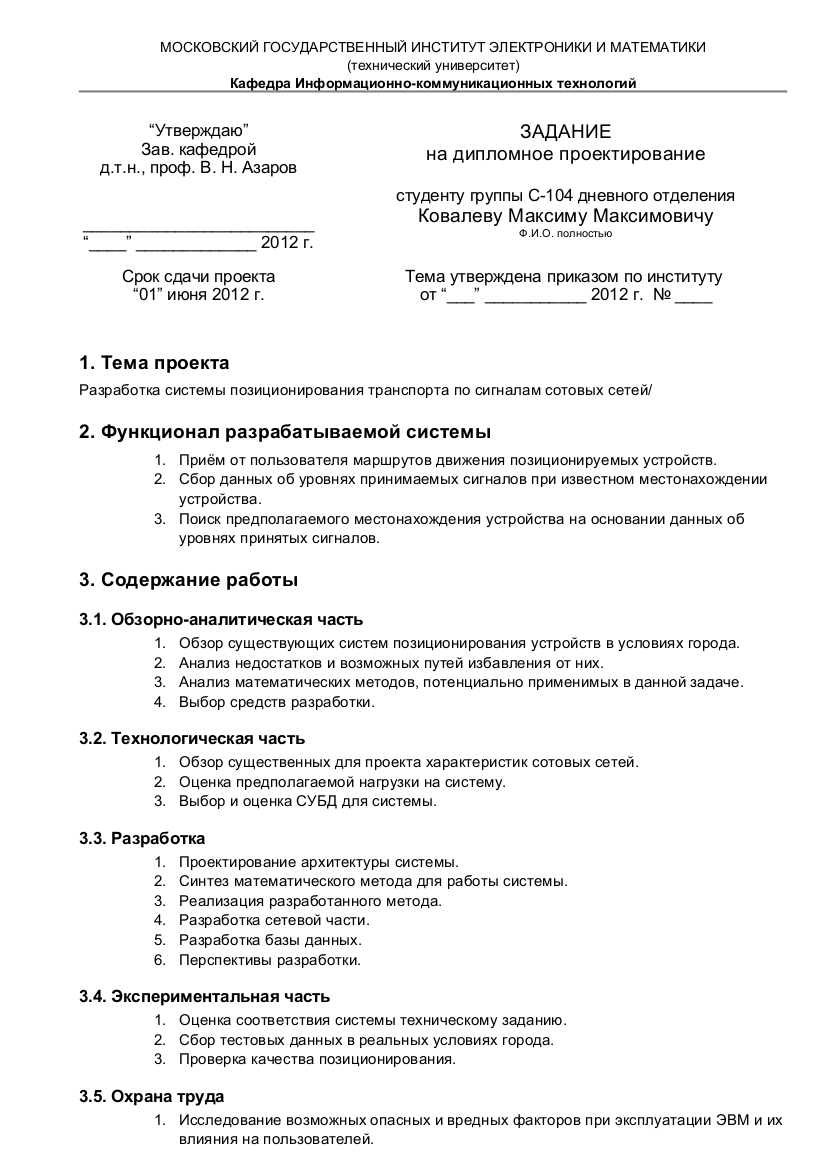
\includegraphics{task-kovalev-page-1.png}%
	\end{textblock*}%
	\null%
	\newpage}

\afterpage{%
	\newpage%
	\thispagestyle{empty}%
	\begin{textblock*}{297mm}(0mm,0mm)%
		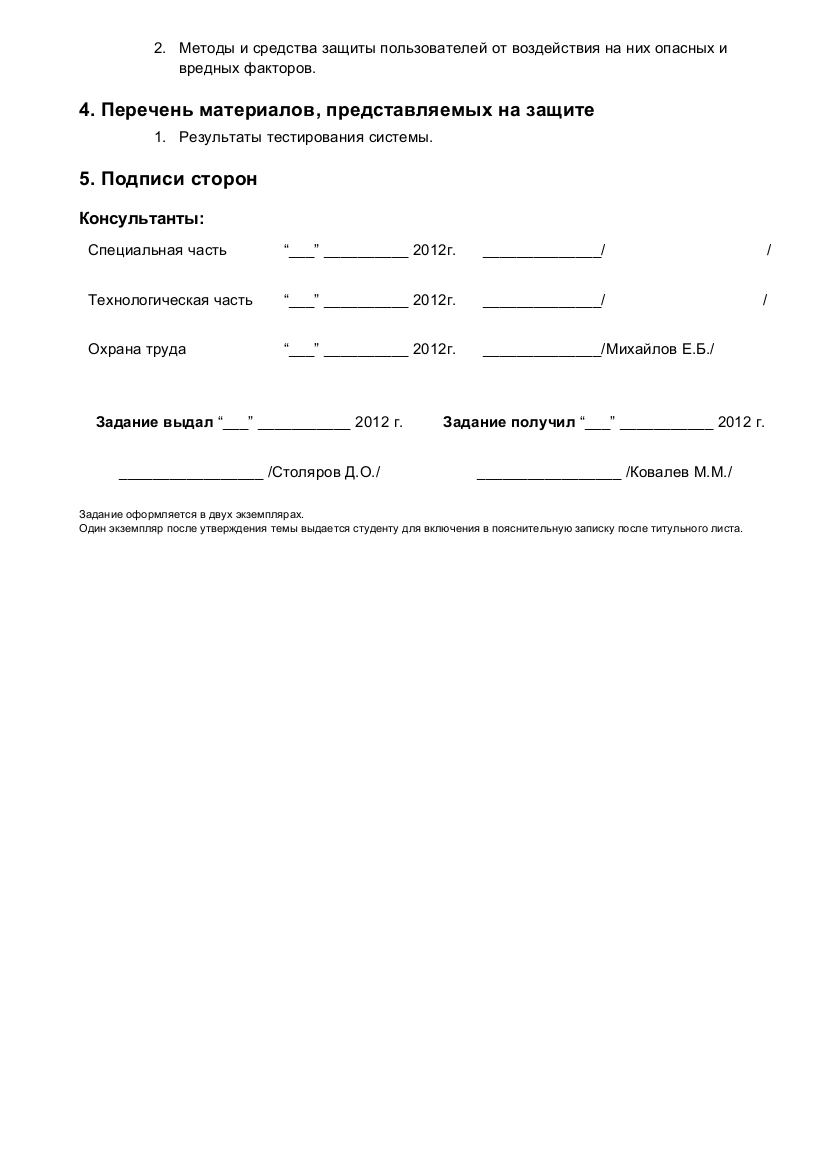
\includegraphics{task-kovalev-page-2.png}%
	\end{textblock*}%
	\null%
	\newpage}

%This file is part of diplom-kovalev
%Copyright (C) 2012 Maxim Kovalev.
%Permission is granted to copy, distribute and/or modify this document
%under the terms of the GNU Free Documentation License, Version 1.3
%or any later version published by the Free Software Foundation;
%with no Invariant Sections, no Front-Cover Texts, and no Back-Cover Texts.
%A copy of the license is included in the section entitled "GNU
%Free Documentation License".

\chapter*{Аннотация}
\addcontentsline{toc}{chapter}{Аннотация}

В данной работе создан и проверен новый метод позиционирования мобильных устройств на основе информации о принимаемых ими уровнях сигналов от базовых станций сетей GSM, рассчитанный на стационарную установку позиционируемых устройств на наземном общественном транспорте. Использование априорной информации о неизменном маршруте движения каждого транспортного средства позволило свести задачу от двухмерной (поиск широты и долготы) к одномерной (поиск расстояния от фиксированной точки на маршруте) и полностью отказаться от применения метода триангуляции в пользу статистического подхода.

Разработанный алгоритм был реализован в прототипе системы позиционирования, после чего проверен на тестовом отрезке пути в реальных городских условиях. Достигнута средняя погрешность определения положения в 49 метров, что лучше, чем у современных систем, основанных на триангуляции, но ещё не позволяет сравниться с системами спутниковой навигации, а потому для достижения возможности внедрения наравне со спутниковыми системами, требуется дополнительная научная и техническая работа.

Исходные коды компонентов разработанной системы, текстовые журналы экспериментов, а также исходные коды данной пояснительной записки в форматах \LaTeX{} и Graphviz вместе с использованными растровыми изображениями доступны в репозитории Subversion по адресу http://svn.auditory.ru/repos/tatmon.

В соответствие с GNU Free Documentation License\cite{gnufdl}, данная работа является свободным документом:
\bigskip
\begin{quote}
    Copyright \copyright{}  2012  Maxim Kovalev.
    Permission is granted to copy, distribute and/or modify this document
    under the terms of the GNU Free Documentation License, Version 1.3
    or any later version published by the Free Software Foundation;
    with no Invariant Sections, no Front-Cover Texts, and no Back-Cover Texts.
\end{quote}
\bigskip


\tableofcontents		% это оглавление, которое генерируется автоматически
\chapter{Введение}

{\bf Актуальность.} На рубеже нулевых и десятых годов XXI века, параллельно идущие процессы удешевления как средств, так и услуг мобильного доступа в сеть Интернет, а также удешевления и миниатюризации средств спутниковой навигации привели к появлению принципиально нового вида онлайн-услуг --- служб, основанных на местоположении (location-based service, LBS)\cite{ruwikilbs}. Одним из таких сервисов является удалённое наблюдение за местонахождением транспортных средств, с помощью установленных на них автономных <<маяков>>, различными способами определяющих собственное местонахождение и передающих данные о нём через мобильный интернет. Владельцы личных автомобилей преимущественно используют подобные средства в следящих противоугонных системах\cite{enwikivetrasy}, но эти средства применимы и в городском транспортном хозяйстве. Помимо непосредственно городских властей, в чьи интересы входит наблюдение за транспортными потоками для задач городского планирования, пресечения злоупотребления служебным положением со стороны недобросовестных водителей и прочих глобальных целей, подобные данные могут быть интересны и простым пассажирам. В связи с трудностью прогнозирования транспортной обстановки, реальный график движения наземного общественного транспорта в часы пик может существенным образом отличаться от расписания. Наблюдение же реальной динамики движения позволило бы создать систему, делающую динамически изменяющиеся прогнозы фактического времени прибытия транспорта и предполагаемого времени в пути, о результатах которого уведомляющую пассажиров через такие каналы как электронные табло на остановках и в самих транспортных средствах, через беспроводную связь подключённые к серверу системы, web-сервис, доступный через стационарные или планшетные компьютеры, приложение для смартфонов (см. рис. \ref{fig:yakazan}), SMS или USSD сервис для любого типа мобильных телефонов и другие. Подобные системы уже начинают внедрять по всему миру\cite{itsrapidbus}\cite{spbtrans}\cite{novosib}\cite{yakazan}, однако по-прежнему сравнительно высокая стоимость приёмников GPS и ГЛОНАСС тормозит процесс внедрения. С другой стороны, существуют сервисы позиционирования мобильных телефонов, использующие для своей работы только информацию о сигналах от базовых станций сотовой сети, но их проблемой является недостаточная точность позиционирования. При этом, на общественном транспорте используются те же системы, что и на личном, хотя между ними есть огромная разница: общественный транспорт движется по заранее известным и неизменным маршрутам, что фактически позволяет свести задачу его позиционирования от двухмерного случая к одномерному. Но эта технологическая ниша оказалась фактически незанятой.

\begin{figure}[h]
	\center{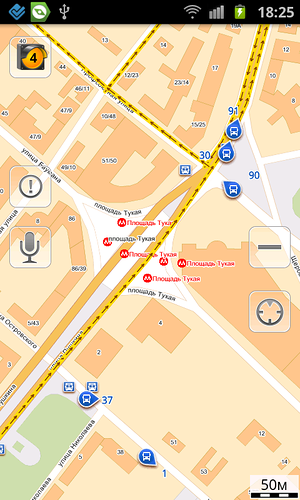
\includegraphics[width=0.5\linewidth]{yakazan.png}}
	\caption{Приложение от Яндекс, в реальном времени показывающее автобусы Казани. Изображение из блога Яндекса\cite{yakazan}}
	\label{fig:yakazan}
\end{figure}

{\bf Целью} данной работы является проверка предположения о возможности существенного повышения точности позиционирования транспортных средств, по сравнению с существующими универсальными системами, при условии заранее известного маршрута движения, а также удешевления подобной системы, по сравнению со случаем использования спутниковой навигации. Для достижения этой цели требуется создать и протестировать прототип подобной системы позиционирования, который, в случае успеха, в дальнейшем может быть доработан до промышленного образца, внедрён и коммерциализирован, однако эти цели уже выходят за рамки данной работы.

{\bf Задачи}, которые требуется решить на пути к данной цели, таковы:

\begin{itemize}
	\item
		Формулировка одномерной задачи позиционирования на местности;
	\item
		Анализ принципов работы существующих систем позиционирования и поиск в них избыточности относительно одномерной задачи позиционирования;
	\item
		Создание математического метода, устраняющего указанную избыточность в пользу большей точности;
	\item
		Проектирование архитектуры системы с учётом разработанного метода и реализация её прототипа:
	\item
		Тестирование созданного прототипа.
\end{itemize}

{\bf Публикации.} Помимо данной пояснительной записки, результаты данной работы также были дважды представлены на разных стадиях на конференции студентов, аспирантов и молодых специалистов МИЭМ (см. <<\nameref{chap:publications}>> на стр. \pageref{chap:publications}). Данная работа также выиграла конкурс грантов <<Участник Молодёжного Научно-Инновационного Конкурса>> в марте 2011 года\cite{umnikwinners}.

\chapter{Обзорно-аналитическая часть}
\section{Существующие системы позиционирования}
На сегодняшний день, наибольшее распространение получили\cite{ruwikilbs} два вида систем позиционирования: основанные на спутниковой навигации и основанные на принимаемых уровнях сигналов от базовых станций сотовых сетей.

\subsection{Спутниковая навигация}
\label{subsec:satnav}
Спутниковые системы позиционирования, такие как GPS и ГЛОНАСС, в качестве опорных точек используют орбитальную группировку спутников, специально запущенных для целей навигации. Орбитальные элементы для всех спутников известны, а потому вычислить местонахождение каждого из них в любой момент времени возможно с большой точностью. После того, как они вычислены, можно осуществлять непосредственно позиционирование.

\begin{figure}[h]
	\center{
		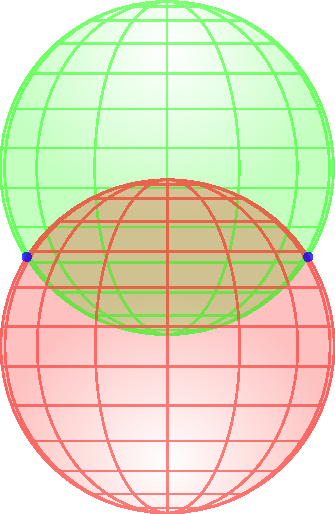
\includegraphics[width=0.4\linewidth]{Lat_2spheres_2.pdf}
		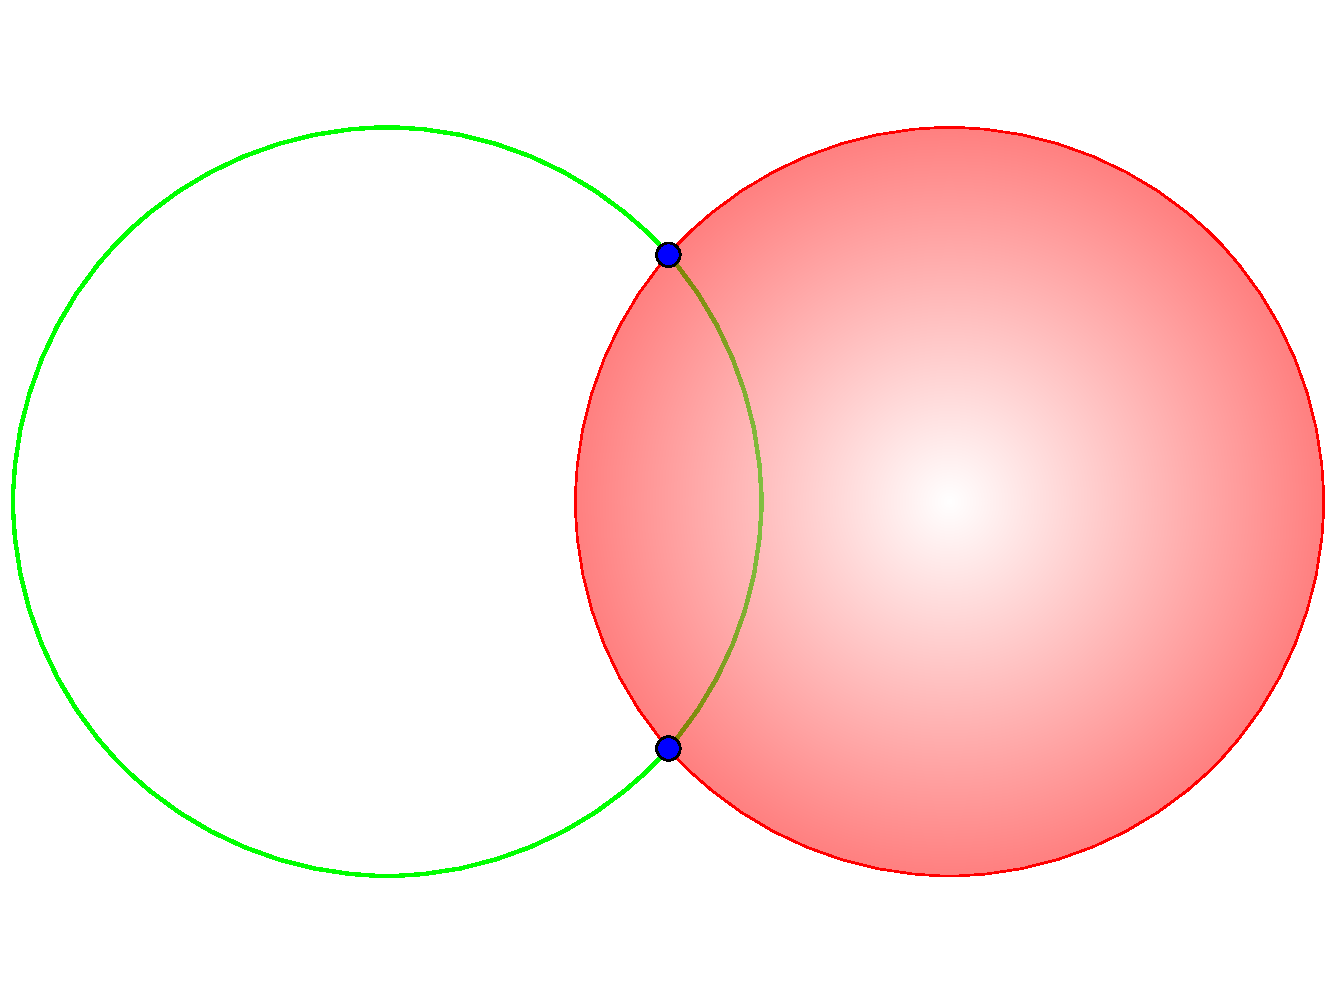
\includegraphics[width=0.4\linewidth]{Circle_sphere_2-colour.pdf}
	}
	\caption{Две пересекающиеся сферы образуют окружность. Третья сфера, пересекая эту окружность, образует две точки. Изображения из фонда Wikimedia Commons.}
	\label{fig:2-3-spheres-intersect}
\end{figure}
GPS использует метод трилатерации, в котором измеряется расстояние от приёмника до трёх видимых спутников. Три сферы, пересекаясь, дают две возможные точки, причём расположенные на разной высоте (см. рис. \ref{fig:2-3-spheres-intersect}), а потому правильной считается ближайшая к поверхности Земли. Для измерения расстояния оценивается время прохождения сигнала от спутника до приёмника. Средняя высота орбит спутников GPS над поверхностью Земли составляет порядка $2\cdot10^7$ метров\cite{enwikigps}, что, с учётом скорости света, равной $3\cdot10^8$ м/с, даёт характерное время прохождения сигнала около 60 миллисекунд. Чтобы при таком порядке задержки обеспечить достаточную точность позиционирования, все спутники оборудованы синхронизированными атомными часами, дающими точность около 14 наносекунд\cite{enwikigps}, причём для её обеспечения приходится учитывать эффекты специальной теории относительности, применительно к движению спутника. Было бы крайне дорого обеспечивать каждый приёмник такими же часами, а потому точное время он вычисляет каждый раз, когда принимает сигнал от спутника, решая уравнения метода трилатерации и относительно положения, и относительно времени.

В случае, когда в области видимости находится более, чем 4 спутника, система уравнений, описывающих положение приёмника, становится избыточной, количество уравнений превышает количества неизвестных. В этом случае, с одной стороны, можно выбрать набор спутников, использование которых даёт наибольшую точность позиционирования, оценивая величину геометрического ухудшения точности (geometric dilution of precision --- GDOP), с другой --- решать избыточную систему уравнений одним из приближённых численных методов, таких как метод наименьших квадратов, чтобы получить лучшую оценку положения автоматически\cite{enwikigps}.

Характерное же расстояние от мобильного устройства до базовой станции сотовой сети, в зависимости от стандарта, составляет $10^2$--$10^4$ метров. Для обеспечения соответствующей точности трилатерации в таких сетях, потребовалось бы пропорционально снизить погрешность точного времени, что представляется трудноосуществимым, поскольку для синхронизации часов базовых станций используется как раз сигнал GPS\cite{gsmclockcalibr}. В связи с этим, в отсутствие возможности использования сигнала GPS (отсутствие приёмника или видимости спутников), применяются иные методы.

\subsection{Позиционирование в сотовых сетях}
Как было показано в пункте \ref{subsec:satnav}, метод оценки расстояния между источником и приёмником, с помощью измерения задержки прохождения сигнала для сотовых сетей неприменим. Однако, остаётся возможность измерить амплитуду принимаемого сигнала, убывающую обратно пропорционально квадрату расстояния. Стандартный GSM-модуль может предоставить информацию об амплитуде принимаемого сигнала не только от базовой станции, через которую идёт передача данных, но и обо всех окружающих, сигнал которых можно принять. Информация эта представляется в виде логарифмической величины received signal strength indicator (RSSI), преобразованную из стандартной единицы измерения --- децибел мощности (dBm) --- в дискретную единицу измерения asu, представляющую из себя целое число в диапазоне от 0 до 31, где 0 соответствует самому малому уровню сигнала, доступному в шкале, а 31 --- самому большому\cite{androidnecelinf}.

\subsubsection{Распространение сигнала на открытой местности}
Максимальный радиус действия одной базовой станции в сети GSM составляет 35 километров на открытой местности, а в условиях городской застройки плотность их расстановки может составлять вплоть до одной станции на 400 метров\cite{enwikicellsite}. Максимальная излучаемая мощность базовой станции стандарта DCS 1800 составляет 40 Вт\cite{gsmts}. Длина волны частотой 1800 МГц составляет $3\cdot10^8\text{(м/с)}/1800\cdot10^6\text{(Гц)} = 16\text{(см)}$. Примем эту величину за характерный размер излучателя и вычислим плотность потока электромагнитного излучения, считая, что 40 Вт излучения проходят через сферу диаметром 16 см:
\begin{equation}
	\label{eq:40wdensity}
	\frac{40\text{(Вт)}}{\pi\cdot0,16^2\text{(м)}} = 497\text{(Вт/м}^2\text{)}
\end{equation}
Отсюда, зависимость мощности излучения от расстояния до базовой станции составит:
\begin{equation}
	\label{eq:p40ofr}
	P = \frac{40^2}{497\cdot{}\pi{}\cdot{}R^2}
\end{equation}
Построим график этой зависимости.

\begin{figure}[h]
	\center{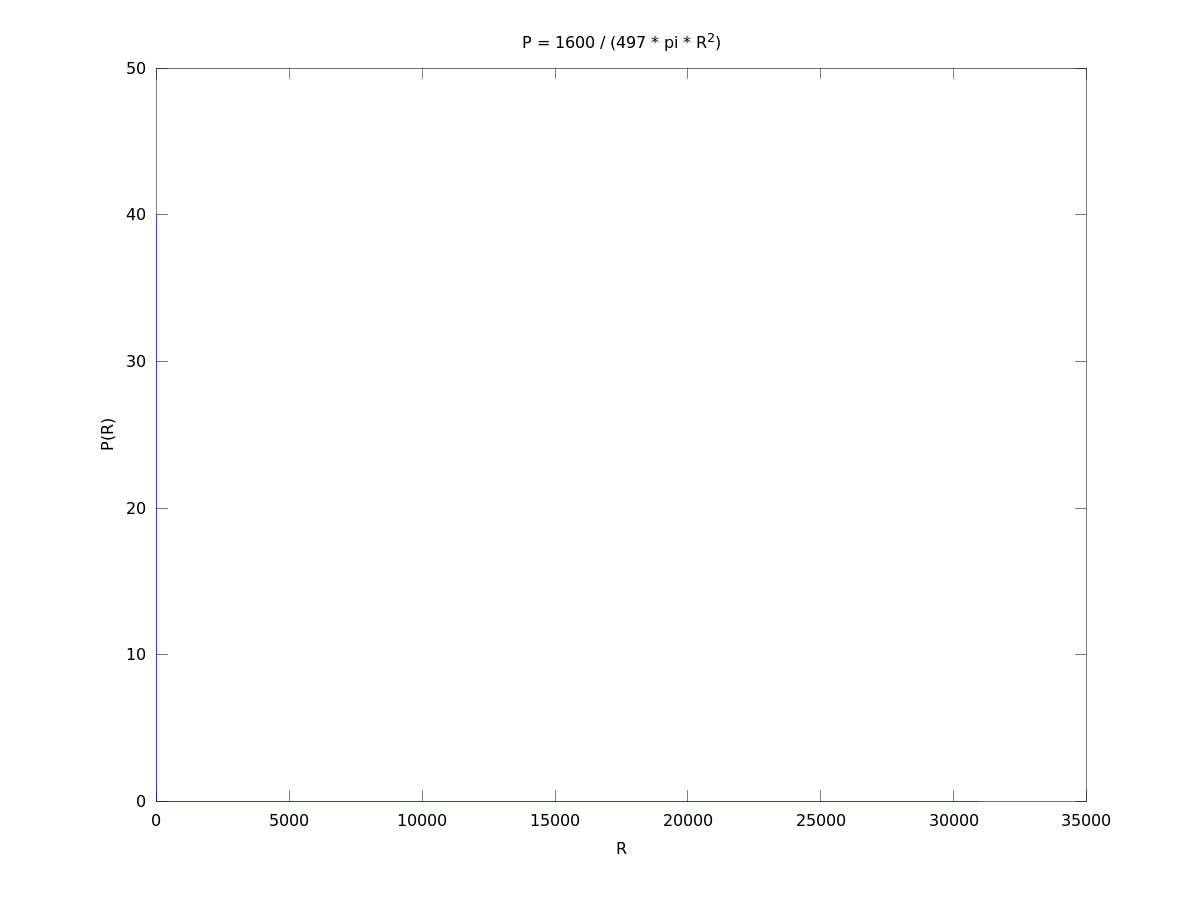
\includegraphics[width=1\linewidth]{bs40wp.png}}
	\caption{Зависимость мощности излучения в ваттах от расстояния в метрах до базовой станции GSM DCS 1800 мощностью 40 Вт. Гипербола столь быстро сходится к асимптотам, что на рисунке сливается с осями координат.}
	\label{fig:bs40wp}
\end{figure}

На рис. \ref{fig:bs40wp} видно, что мощность, измеренная в ваттах, близка к нулю для всех 35 возможных километров. В связи с этим, целесообразно введение логарифмической величины децибел мощности (dBm), связанной с ваттом следующим соотношением\cite{enwikidbm}:
\begin{equation}
	\label{eq:wtodbm}
	x = 10\cdot{}\log_{10}(1000\cdot{}P)
\end{equation}
Подставим формулу \ref{eq:p40ofr} в \ref{eq:wtodbm} и построим график получившейся зависимости.

\begin{figure}[h]
	\center{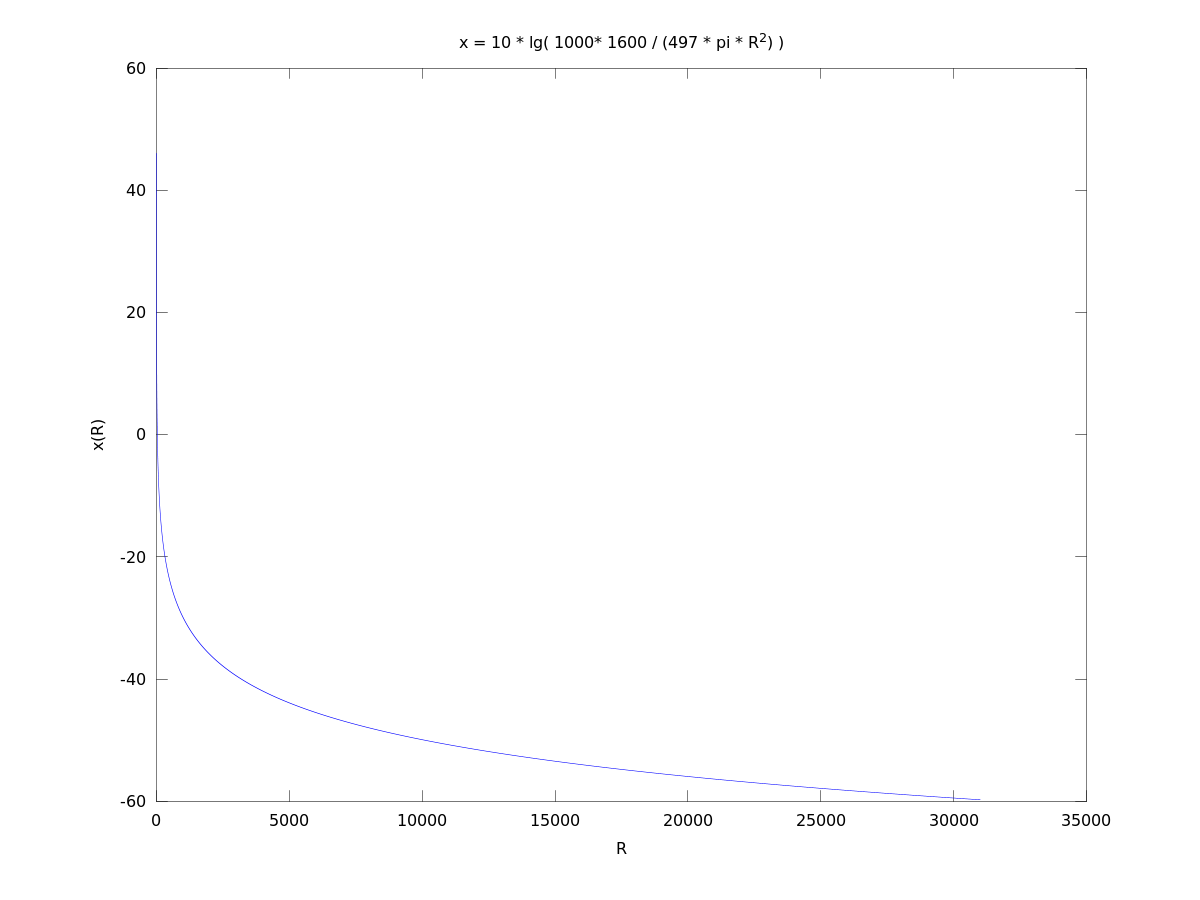
\includegraphics[width=1\linewidth]{bs40wdbm.png}}
	\caption{Зависимость мощности излучения в децибелах мощности от расстояния в метрах до базовой станции GSM DCS 1800 мощностью 40 Вт.}
	\label{fig:bs40wdbm}
\end{figure}

На рис. \ref{fig:bs40wdbm} видно, что использование логарифмического масштаба позволяет получить кривую, намного более равномерно заполняющую координатную плоскость, чем в линейном масштабе как на рис. \ref{fig:bs40wp}.

Наконец, возьмём связь между единицами dBm и asu\cite{androidnecelinf}:
\begin{equation}
	\label{eq:dbmtoasu}
	\text{asu} = \frac{\text{dBm} + 113}{2}
\end{equation}
Подставим формулы \ref{eq:p40ofr} и \ref{eq:wtodbm} в \ref{eq:dbmtoasu} и получим:
\begin{equation}
	\label{eq:p40rtoasu}
	\text{asu} = \frac{10\cdot{}\log_{10}(1000\cdot{}\frac{40^2}{497\cdot{}\pi{}\cdot{}R^2}) + 113}{2}
\end{equation}

\subsubsection{Погрешность определения расстояния}
Рассмотрим формулу \ref{eq:p40rtoasu} и найдём, на каких расстояниях от базовой станции будет меняться asu.
\begin{table}
	\caption{\label{tab:asuchange}Расстояния до точек изменения asu от базовой станции GSM DCS 1800 мощностью 40 Вт. Теоретическая оценка.}
	\begin{center}
		\begin{tabular}{|p{0.2\linewidth}|l|p{0.2\linewidth}|p{0.3\linewidth}|}
			\hline
			Расстояние от станции, метров & Значение asu & Расстояние до следующей точки изменения asu & Отношение расстояния до следующей точки изменения asu к расстоянию от станции \\
			\hline
			143 & 50 & 37 & 0.259 \\
			\hline
			180 & 49 & 47 & 0.261 \\
			\hline
			227 & 48 & 58 & 0.255 \\
			\hline
			285 & 47 & 74 & 0.260 \\
			\hline
			259 & 46 & 93 & 0.259 \\
			\hline
			359 & 46 & 93 & 0.259 \\
			\hline
			452 & 45 & 117 & 0.259 \\
			\hline
			569 & 44 & 148 & 0.260 \\
			\hline
			717 & 43 & 185 & 0.258 \\
			\hline
			902 & 42 & 234 & 0.259 \\
			\hline
			1136 & 41 & 294 & 0.259 \\
			\hline
			1430 & 40 & 370 & 0.259 \\
			\hline
			1800 & 39 & 466 & 0.259 \\
			\hline
			2266 & 38 & 587 & 0.259 \\
			\hline
			2853 & 37 & 739 & 0.259 \\
			\hline
			3592 & 36 & 930 & 0.259 \\
			\hline
			4522 & 35 & 1170 & 0.259 \\
			\hline
			5692 & 34 & 1475 & 0.259 \\
			\hline
			7167 & 33 & 1856 & 0.259 \\
			\hline
			9023 & 32 & 2336 & 0.259 \\
			\hline
			11359 & 31 & 2941 & 0.259 \\
			\hline
			14300 & 30 & 3700 & 0.259 \\
			\hline
			18000 & 29 & 4660 & 0.259 \\
			\hline
			22660 & 28 & 5870 & 0.259 \\
			\hline
			28530 & 29 & & \\
			\hline
		\end{tabular}
	\end{center}
\end{table}
В таблице \ref{tab:asuchange} для наглядности мы намеренно пренебрегли ограничением на максимальное значение asu, равное 31, и это допустимо, поскольку при использовании базовой станции с меньшей мощностью передатчика, значения asu также сдвинутся в меньшую сторону, и допустимый диапазон asu будет достигаться не на границе радиуса действия базовой станции, а в его середине или начале.

\begin{figure}[h]
	\center{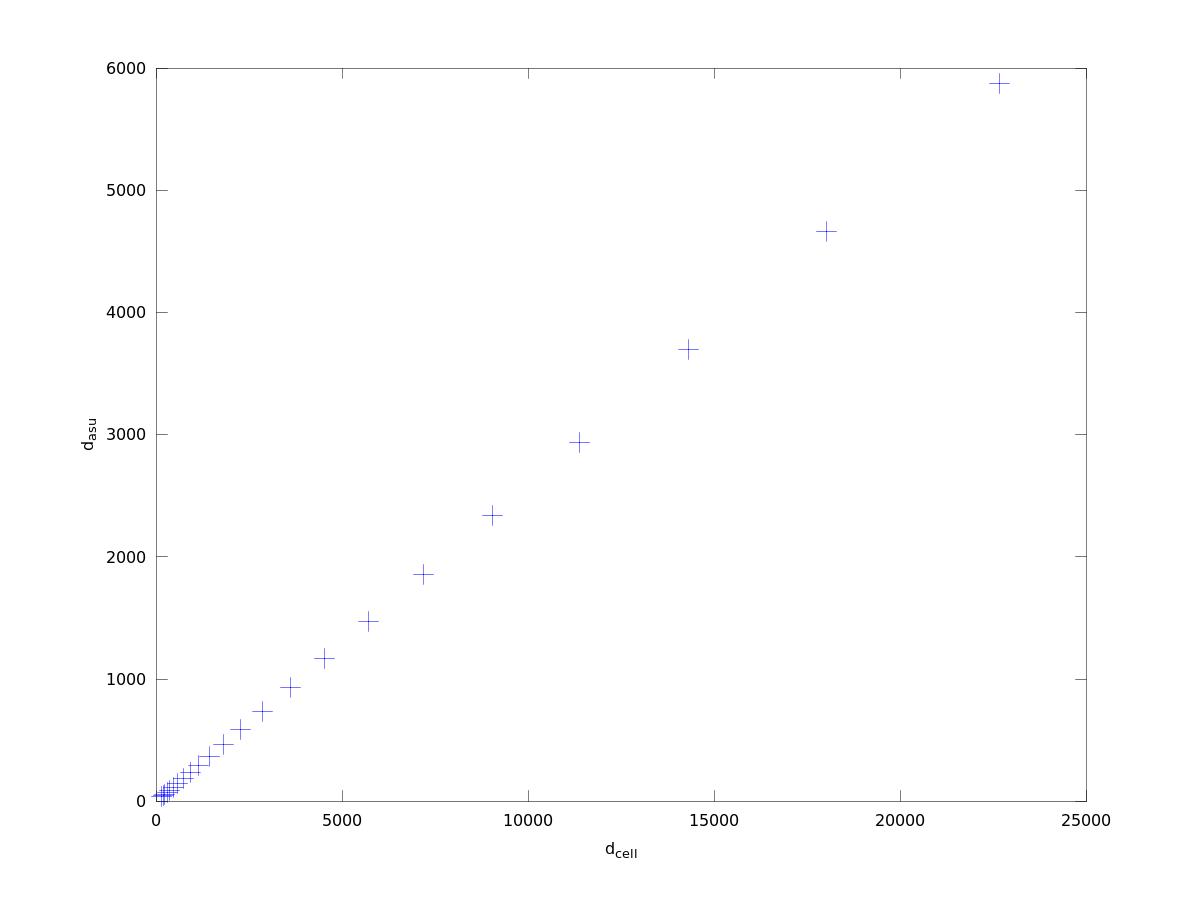
\includegraphics[width=1\linewidth]{dcelldasu.png}}
	\caption{Зависимость расстояния между двумя точками, где asu принимает целочисленное значение, от расстояния этих точек до базовой станции, по осям отложены метры}
	\label{fig:dcelldasu}
\end{figure}

Поскольку GSM-модуль передаёт для дальнейшей обработки только целую часть asu, расстояние между двумя соседними точками, где asu на самом деле имеет целое значение, можно считать погрешностью изменения расстояния на этом интервале. А так как измеряемой величиной является расстояние до базовой станции, отношение длины этого интервала к расстоянию до неё будет относительной погрешностью измерения. Из таблицы \ref{tab:asuchange} видно, что относительная погрешность остаётся постоянной на любом расстоянии. На рис. \ref{fig:dcelldasu} наглядно показано, что абсолютная погрешность при этом, как и следует ожидать, зависит от расстояния линейно.

При этом, стоит заметить, что эти значения погрешности были вычислены в предположении, что единственным фактором, ограничивающим точность измерений, является <<цена деления>> GSM-модуля, измеряющего asu. Однако в реальности, следует ожидать вмешательства случайной погрешности. Если считать, что в некоторой местности уровень электромагнитных помех примерно одинаков для любой точки, то с ростом расстояния до базовой станции отношение сигнал/шум будет падать, что внесёт дополнительную погрешность.

Таким образом, видно, что измерение расстояния от базовой станции до мобильного устройства, основанное на амплитуде сигнала, позволяет достигнуть точности от десятков метров до единиц километров, в зависимости от расстояния до базовой станции и мощности её передатчика. Наибольшая точность достигается вблизи станции, но при условии, что измеренное значение RSSI, выраженное в единицах asu, не выходит за пределы допустимого диапазона.

\subsubsection{Координаты базовых станций}
Для определения абсолютного местоположения мобильного устройства, а не только его положения относительно некоторых опорных точек, требуется знать координаты самих опорных точек. В случае использования спутниковой навигации, спутники немногочисленны --- на 24.05.2010 их было 31\cite{enwikigps} на всю Землю --- а их координаты в любой момент времени можно рассчитать с помощью законов орбитальной механики. В случае же базовых станций сотовых сетей, их количество для одной только России на конец 2011 года превысило 165 тысяч\cite{decodcells}. При этом, популярными провайдерами геолокационных сервисов зачастую являются не сотовые операторы, а сторонние компании, такие как Google, предоставляющий сервис Google Latitude, или Яндекс.Локатор от компании Яндекс\cite{ruwikilbs}. Такие провайдеры могут работать в зонах покрытия множества различных операторов сотовой связи, а также, при наличии соответствующего приёмного оборудования на мобильном устройстве, использовать для повышения точности позиционирования и другие беспроводные сети, такие как WiFi или WiMAX\cite{geolocationapidata}\cite{googlocsource}. 

В связи с этим, у провайдера геолокационного сервиса обычно нет априорных данных о координатах базовых станций, которые используются для позиционирования. Работа любой подобной системы начинается с того, что измеряются RSSI видимых базовых станций во множестве точек на местности, координаты которых получаются с помощью спутниковой навигации. Когда достаточное количество подобных замеров осуществлено, решается обратная задача -- вместо позиционирования устройства по известным координатам базовых станций, приближённо вычисляются координаты базовых станций, при известных координатах точек замеров RSSI.\cite{talberg}. Также распространена ситуация, в которой данные о координатах базовых станций уточняются непосредственно в процессе работы системы. В этом случае, провайдеры изыскивают способы вынудить самих пользователей сервиса посылать данные, помогающие уточнить базу данных. Так, пользовательское соглашение сервиса Яндекс.Локатор требует обязательной посылки данных нетмониторинга в случае, если от пользователя к сервису поступает более тысячи запросов в день\cite{yaloceula}.

Поскольку предполагаемые координаты базовых станций представляют собой большой объём данный, к тому же, постоянно изменяющийся, они хранятся не на позиционируемом устройстве, а на сервере провайдера геолокационного сервиса. Таким образом, само устройство вычислить свои координаты не может, оно лишь отправляет запрос с результатами измерений на сервер, откуда получает ответ о предполагаемом местонахождении\cite{yageloc}. Поэтому для работы таких систем обязательно наличие подключения к интернету.

Отсюда следует, что:

\begin{enumerate}
	\item
		Подобные системы являются самообучающимися: чем больше их используют, тем точнее они работают;
	\item
		Подобные системы могут работать только в тех местах, где кто-то ранее измерял RSSI и посылал эти данные провайдеру вместе с определёнными по GPS координатами точки измерения.
\end{enumerate}

\subsubsection{Факторы, снижающие точность позиционирования}
\label{subsubsec:pospreclow}
Реальные условия работы системы могут существенным образом отличаться от рассмотренного случая. В силу ряда факторов, системы позиционирования в мобильных сетях не достигают такой точности, как спутниковые. В отличие от спутниковых систем, сигналы точного времени которых могут быть либо приняты, либо нет, а на время прохождения сигнала влияет только расстояние, уровень сигнала от станций сотовых сетей подвержен множеству аналоговых искажений. Сюда можно включить:

\begin{enumerate}
	\item
		Поглощение излучения городской застройкой, деревьями, атмосферными осадками;
	\item
		Частичное отражение излучения от городской застройки, в результате которого сигнал от базовой станции достигает мобильного устройства не по прямой, а по ломанной, причём иногда, в результате частичного отражения, одновременно несколькими путями;
	\item
		Волновые эффекты распространения сигнала между домами и воздушными силовыми и сигнальными кабелями, которые могут работать как волноводы;
	\item
		Анизотропия диаграммы направленности базовых станций, в связи с которой на одном и том же расстоянии от неё, но в разных точках, RSSI может быть разным;
	\item
		Анизотропия диаграммы направленности мобильных устройств, в связи с которой одно и то же устройство в одном и том же месте может показывать различные RSSI для всех окружающих базовых станций, в зависимости от своей ориентации в пространстве;
	\item
		Помехи на частотах работы базовых станций.
\end{enumerate}

Эти и многие другие факторы могут приводить сразу к двум негативным последствиям:

\begin{enumerate}
	\item
		На этапе сбора данных, искажённые RSSI приведут к ошибочному определению координат базовых станций:
	\item
		На этапе позиционирования мобильных устройств, точность будут снижать и ошибки в определении текущих уровней сигналов, и ранее накопленные ошибки позиционирования базовых станций.
\end{enumerate}

\subsection{Заключение}
\begin{table}
	\caption{\label{tab:gpsvslbs}Сравнение свойств спутникового позиционирования и позиционирования в сотовых сетях}
	\begin{center}
		\begin{tabular}{|p{0.2\linewidth}|p{0.3\linewidth}|p{0.3\linewidth}|}
			\hline
			Характеристика & GPS & Сотовые сети \\
			\hline
			Опорные точки & Десятки спутников на околоземных орбитах & Сотни тысяч стационарных базовых станций \\
			\hline
			Метод определения расстояния & Измерение задержки прохождения сигнала & Измерение затухания амплитуды сигнала \\
			\hline
			Координаты опорных точек & Известны с большой точностью & Необходимо приблизительно оценивать с помощью дополнительных измерений \\
			\hline
			Погрешность позиционирования & Единицы--десятки метров, зависит от видимости спутников & Десятки--сотни метров, зависит от множества факторов \\
			\hline
			Покрытие & Всемирное & Только там, где проводились предварительные замеры сигнала \\
			\hline
			Автономность устройства & Для работы достаточно приёмника & Нужен обмен данными с сервером провайдера \\
			\hline
			Условие прохождения сигнала & Нахождение под открытым небом с таким углом обзора, чтобы были видны хотя бы три спутника & Везде, где есть сотовая связь \\
			\hline
		\end{tabular}
	\end{center}
\end{table}

В таблице \ref{tab:gpsvslbs} сведены характеристики, рассмотренные в данном разделе. Видно, что спутниковая навигация выигрывает у позиционирования в сотовых сетях практически по всем параметрам. К её недостаткам можно отнести необходимость нахождения под открытым небом для работы спутниковой навигации, а в случае использования в автономных устройствах --- наличие приёмника GPS помимо и так необходимого модуля GSM, что повышает стоимость и энергопотребление прибора.

\section{Позиционирование общественного транспорта}

Позиционирование транспортных средств с помощью установленных на них автономных <<маяков>> является частным случаем задачи позиционирования мобильных устройств. В случае работы с легковыми и грузовыми автомобилями, требования не будут существенно отличаться от задачи позиционирования мобильного телефона или навигатора. Однако, если речь идёт об общественном транспорте, в задаче появляется новая сущность --- маршрут, от движения по которому транспортное средство не может отклоняться.

Трамвай не может отклониться от маршрута вообще, троллейбус --- не более, чем на длину штангового токоприёмника, автобус --- на ширину проезжей части. Иными словами, задачу позиционирования общественного транспорта можно считать практически одномерной. Для каждого транспортного средства маршрут движения известен заранее, определять его не требуется. Таким образом, возможность позиционирования устройства в произвольном месте двухмерной карты является избыточной по отношению к данной задаче.

\subsection{Снижение точности из-за двухмерной избыточности}
\label{subsec:2dlowprec}
\begin{figure}[h]
	\center{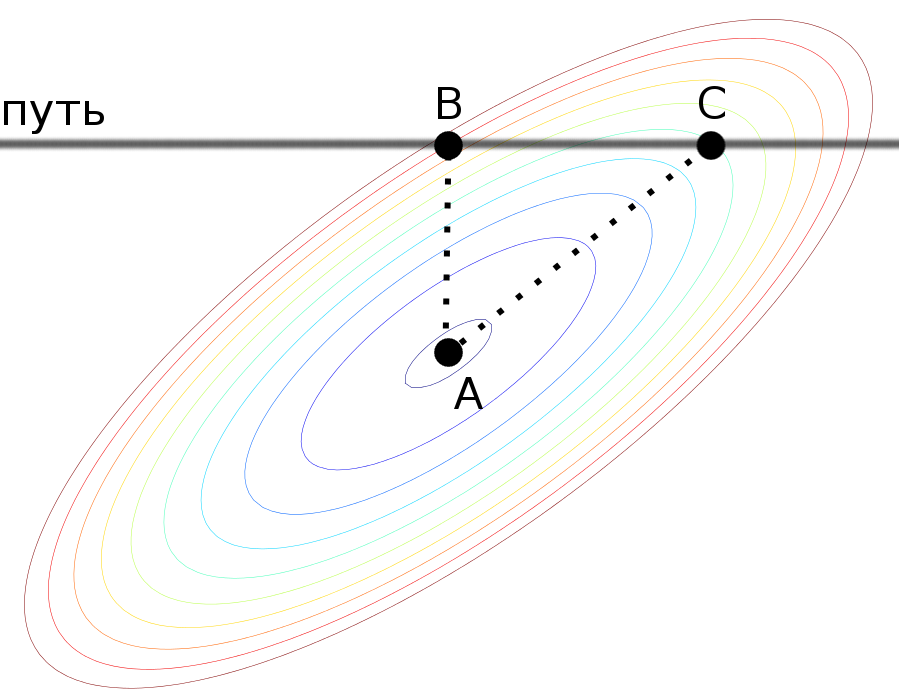
\includegraphics[width=1\linewidth]{contour.png}}
	\caption{Возможная ситуация при позиционировании транспорта. Изолинии показывают целевую функцию метода наименьших квадратов. Точка A --- глобальный минимум, она будет считаться результатом позиционирования. B --- проекция минимума на путь, по которому движется транспортное средство. C --- точка на пути движения, в которой достигается наименьшее значение целевой функции.}
	\label{fig:contour}
\end{figure}

Рассмотрим случай движения транспортного средства по прямой и позиционирования на ней. Как было отмечено в пункте \ref{subsec:satnav}, в случае, когда имеются избыточные данные о расстояниях до опорных точек, применяются различные методы приближённого решения, такие как метод наименьших квадратов. Конечным этапом применения такого метода будет определение для каждой точки на карте целевой функции, выражающей степень неуверенности в том, что данная точка является искомой, и поиск глобального минимума этой функции\cite{enwikiols}. На рис. \ref{fig:contour} изображено одно из возможных взаимных расположений пути следования транспортного средства и целевой функции. Глобальный минимум, который геолокационный сервер выдаст в качестве ответа на запрос местоположения, из-за ошибок измерения, находится в точке A, не лежащей на маршруте, хотя на самом деле, истинное положение находится где-то на маршруте. Если нам дана только точка A и маршрут движения, то наилучшим приближением будет проекция точки A на маршрут --- точка B. Однако, если учесть маршрут движения ещё на этапе, когда доступными являются все значения целевой функции, а не только информация о расположении минимума, то можно вычислить точку C, рассмотрев все точки, лежащие на маршруте, и найдя среди них такую, для которой значение целевой функции минимально, и это будет лучшим приближением.

\subsection{Снижение точности из-за экстраполяции}
\label{subsec:extralowprec}
Как было отмечено в подпункте \ref{subsubsec:pospreclow}, ошибки в ходе позиционирования возникают сразу на двух этапах: и на этапе составления карты базовых станций, и на этапе непосредственно позиционирования. Сам метод триангуляции обязывает применять именно такую последовательность действий, однако необходимо обосновать применение триангуляции как таковой. В случае позиционирования ручных и автомобильных устройств, необходимость применения этого метода обусловлена тем, что невозможно измерить уровни принимаемых сигналов во всех точках, где необходимо покрытие геолокационного сервиса. Так, если считать, что для триангуляции достаточно трёх замеров в точках, не лежащих на одной прямой, то для вычисления координат трёх базовых станций, достаточно трёх измерений, если учесть, что их зоны покрытия перекрываются. Три таких замера дадут возможность после этого позиционировать устройства во всей области, где перекрываются зоны покрытия этих станций.

В случае же общественного транспорта ситуация совершенно иная. Для примера рассмотрим московскую трамвайную сеть. На 46 маршрутов приходится 1000 трамваев\cite{ruwikimostram}. Если каждый трамвай хотя бы раз в день полностью проходит свой маршрут, это уже даст $1000/46 = 22$ вагона на одной линии. Приборы, оборудованные системой спутниковой навигации, и собирающие данные об RSSI, будучи установленными всего на один из каждых 22 вагонов, уже дадут полное обновление карты покрытия для каждой точки каждого маршрута.

Необходимости экстраполировать собранные данные на окружающие точки во всём городе в такой ситуации нет. Достаточно осуществить интерполяцию между имеющимися точками в одномерном случае.

\subsection{Гипотеза о возможности повышения точности}
Анализ факторов, изложенных в пунктах \ref{subsec:2dlowprec} и \ref{subsec:extralowprec}, позволяет предположить, что использование свойств, специфичных для наземного общественного транспорта, позволит отказаться от стадий процесса позиционирования, снижающих его точность. В данной работе экспериментально проверяется возможность этого.

\section{Анализ возможности применения существующих алгоритмов}
Рассмотрим, с помощью каких алгоритмов и математических методов можно решать задачу позиционирования, если не использовать триангуляцию.

\subsection{Постановка задачи}
\begin{enumerate}
	\item
		Дана числовая прямая, обозначающая маршрут движения. Задача отображения двухмерных координат на эту прямую решается отдельно;
	\item
		Некоторое количество переменных, выражающих принимаемый уровень сигнала от каждой станции, являются функциями от положения на прямой, определены на всей её длине (отсутствие сигнала можно трактовать как нулевой уровень), но подвержены также случайным флуктуациям;
	\item
		Для ряда точек, случайно расположенных на прямой, даны предварительно измеренные значения переменных. Возможна и ситуация неоднократных замеров в одной точке, давших разные результаты, они все попадают в массив измерений;
	\item
		Для кортежа из нескольких измеренных значений найти точку на прямой, где они с наибольшей вероятностью были осуществлены.
\end{enumerate}

Таким образом, требуется найти алгоритм, который будет способен сравнивать точки на прямой по степени их похожести друг на друга, основываясь на значениях набор дискретных, но упорядоченных переменных (то есть, учитывать то, что, например, 13 больше похоже на 14, чем на 42), устойчивый к выбросам (то есть, если какая-то одна станция неожиданно даст сигнал, резко отличающийся от своего нормального значения, это не должно стать помехой) и учитывающий ситуацию в соседних точках (если в некоторой точке никогда не было зафиксировано некое конкретное значение RSSI, но метром больше и метром ближе --- было, то для данной точки оно также должно быть репрезентативным). Также желательно учесть распределение результатов измерений для каждой точки, хотя подойдёт и использование среднего значения.

Математического метода, удовлетворяющего всем перечисленным требованиям, найдено не было, однако рассмотрим ряд существующих, наиболее приближающихся к заданным требованиям, на основе которых в дальнейшем будет синтезироваться новый.

\subsection{Расстояние Махаланобиса}
\label{subsec:mahalanobis}
Расстояние Махаланобиса --- это обобщение Евклидовой метрики на случай, когда известно, что сравниваемые векторы состоят из случайных переменных\cite{mahalanobis}. Для одного из сравниваемых векторов определяется матрица ковариации его компонентов, таким образом чётко выражена разница между целым набором статистических данных об измерениях, сделанных в конкретной точке, и вектором, однократно измеренным во время позиционирования. В дальнейшем, эта матрица используется для того, чтобы определить величину дисперсии значений в направлении между сравниваемыми векторами. В случае, когда дисперсия мала (то есть, известно, что получение значений, сильно отличающихся от среднего, маловероятно), расстояние получается больше Евклидова, когда велика -- меньше. Определяется расстояние по формуле \ref{eq:mahalanobis}.

\begin{equation}
	D_M(x) = \sqrt{(x - \mu{})^\intercal{}\cdot{}S^{-1}(x-\mu)}
	\label{eq:mahalanobis}
\end{equation}
В формуле \ref{eq:mahalanobis}:
\begin{itemize}
	\item
		{\bf$D_M(x)$} --- расстояние Махаланобиса от вектора $x$ до вектора $\mu$;
	\item
		{\bf$x$} --- однократно измеренный вектор;
	\item
		{\bf$\mu$} --- вектор с известным распределением;
	\item
		{\bf$S$} --- матрица ковариации вектора $\mu$.
\end{itemize}

В поставленной задаче расстояние Махаланобиса можно вычислить для всех точек на маршруте, после чего найти среди них наименьшее --- оно и будет точкой наиболее вероятного местонахождения устройства. Оценивая его применимость, отметим, что такой метод идеально справляется с учётом статистических данных об измеренных уровнях, учитывает упорядоченность множества возможных значений уровней, средне справляется в выбросами: если для какой-то конкретной станции известно, что её сигнал в данной точке нестабилен, она будет учитываться с меньшим весом в конечном результате. Однако если выброс даст <<надёжная станция>>, он в значительной мере изменит оценку.

Главным недостатком является тот факт, что такой метод не позволяет учесть непрерывность самого маршрута. Расстояние Махаланобиса можно определить только для одной точки, не учитывая соседние, либо для интервала, в рамках которого точки будут неразличимыми. Если же в некоторой точке уровни не были измерены никогда, то она никогда не будет результатом позиционирования, даже если есть данные о двух соседних.

\subsection{Байесовский классификатор}
\label{subsec:bayes}
Задача позиционирования по своей сути схожа с задачей классификации: если рассматривать каждую точку на маршруте как класс, то он будет определён имеющимися статическими данными о замерах RSSI в данном месте, а само позиционирование будет отнесением вектора измеренных значений к одному из классов. По этой причине в обзор также включён Байесовский классификатор.

Байесовский классификатор обладает следующими свойствами\cite{akinator}:
\begin{itemize}
	\item
		Строится на основании ранее полученных экземпляров класса, даже если сами экземпляры сильно искажены флуктуациями; сложение большого их количества обеспечивает выявление скрытых закономерностей, характерных для класса;
	\item
		Крайне устойчив к выбросам; мерой веса каждой из переменных является то, в какой мере она уменьшает энтропию распределения вероятности отнесения примера к различным классам, поэтому чем в большей мере нормальные значения переменных свидетельствуют в пользу конкретного класса, тем меньший вес имеют выбросы;
	\item
		Позволяет учесть распределение переменных в экземплярах одного класса.
\end{itemize}

Критическим же недостатком этого классификатора является то, что он рассчитан на дискретные классы и дискретные значения переменных, не позволяя учесть не только соседние точки, но и ближайшие значения RSSI, упорядоченность множества значений переменных тут не учитывается.

С другой стороны, именно как попытка в некотором смысле обобщения Байесовского классификатора на непрерывный случай и был изобретён метод, предлагаемый в данной работе, и Байесовское понимание вероятности как степени уверенности в суждении, а не частоты появления события, легло в его основу.


\chapter{Технологическая часть}

\section{Общая архитектура системы}

\subsection{Процесс обработки данных}

Независимо от того, какой именно математический метод будет осуществлять позиционирование устройства на основе имеющихся данных, можно с уверенностью сказать, что в системе будут поочерёдно или параллельно происходить два процесса: обучение и использование.

Процесс обучения состоит из следующих этапов:

\begin{enumerate}
	\item
		Измерение RSSI видимых базовых станций устройством, оборудованным модулем спутниковой навигации;
	\item
		Передача данных о базовых станциях и положении устройства на сервер;
	\item
		Приём и первоначальная обработка данных сервером. В этот этап могут входить такие процессы как проверка корректности, преобразование координат из пары широта/долгота в пару маршрут/расстояние и так далее;
	\item
		Сохранение собранной информации в базе данных;
	\item
		После набора достаточного количества данных --- вычисление необходимых данных для алгоритма позиционирования (обучение).
\end{enumerate}

Процесс позиционирования проходит следующим образом:

\begin{enumerate}
	\item
		Измерение RSSI видимых базовых станций устройством, не оборудованным модулем спутниковой навигации;
	\item
		Приём данных сервером;
	\item
		Вычисление предполагаемого расположения устройства с помощью обученного алгоритма;
	\item
		Если требуется --- обратное преобразование координат в двухмерные (например, для отображения на карте), хотя этот шаг может и отсутствовать (так, для электронного табло на остановке более подходит именно расстояние по маршруту);
	\item
		Передача данных о положении устройства клиентам.
\end{enumerate}

\subsection{Состав системы}
На основании данного описания логики работы системы, предложена архитектура, изображённая на рис. \ref{fig:general-arch}.

\begin{figure}[h]
	\center{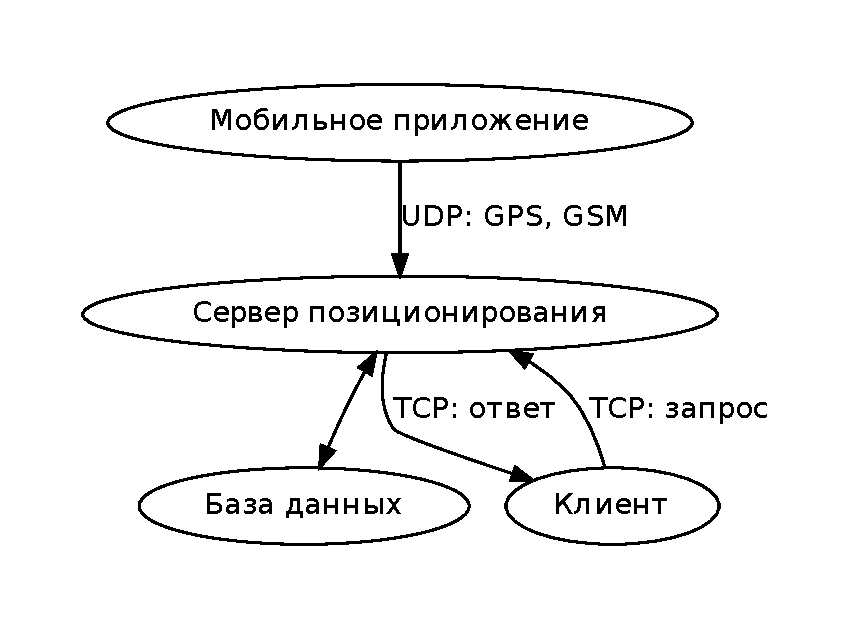
\includegraphics[width=1\linewidth]{general-arch.pdf}}
	\caption{Общая архитектура разрабатываемой системы}
	\label{fig:general-arch}
\end{figure}

Приложение, работающее на мобильном устройстве, в зависимости от типа последнего, передаёт на сервер данные о своём положении и видимых базовых станциях, либо только о базовых станциях. Для передачи используется протокол UDP. Выбор обусловлен тем, что доставка подобных данных не является для системы критичной, а поток данных идёт только в одном направлении.

Связь с клиентами осуществляется по протоколу TCP, причём по запросу клиента. Вызвано это тем, что сервер заранее не обладает информацией о том, куда ему передавать данные, а сами клиенты могут не иметь возможности принять входящее соединение.

\section{Средства разработки}

\subsection{Система контроля версий}
С целью достижения надёжного хранения исходных кодов, возможности получать и изменять код на разных машинах, в том числе и на сервере, возможности отката к предыдущим версиям и предоставления кода всем желающим, была использована система контроля Subversion, официальный кафедральный репозиторий которой находится по адресу http://svn.auditory.ru/.

\subsection{Мобильное приложение}
В качестве как позиционируемого устройства, так и прибора для контрольных замеров RSSI в данной работе использован телефон под управлением операционной системы Android. Данная операционная система имеет удобные средства для работы как с данными об RSSI\cite{androidnecelinf}, так с GPS\cite{androidlocman}. Пользовательские приложения данной ОС исполняются на виртуальной машине dalvik\cite{enwikidalvik}, основным языком программирования для которой является Java, SDK для которой предоставляют разработчики ОС\cite{androidsdk}.

Разработка под Android возможна как и с помощью ручного управления файлами, так и через IDE. Одной из официально поддерживаемых IDE является Eclipse, который и был выбран для разработки.

\subsection{Сервер и СУБД}
Платформой для серверной части был выбран дистрибутив Gentoo Linux, VPS под управлением которого возможно было использовать для тестирования проекта. Имеющаяся там СУБД mysql также подошла для проекта.

Языком программирования был выбран Python. Его стандартная библиотека покрыла все нужды, кроме быстрых вычислений и соединения с базой данных. Для вычислений использовалась библиотека NumPy\cite{numpy}, а для соединения с базой данных --- MySQLdb\cite{mysqldb}. Будучи написанной на интерпретируемом языке и использующей только библиотечные средства взаимодействия с внешними компонентами, программа может работать везде, где имеется интерпретатор языка Python версии не ниже 2.6 с установленными библиотеками NumPy и MySQLdb.

Вместо IDE в разработке данной части применялся консольный текстовый редактор vim\cite{vim}. Он предоставляет огромные возможности для редактирования исходных кодов, а тот факт, что его интерфейс является полностью консольным, позволил использовать его для редактирования кода серверной части непосредственно на VPS через подключение по удалённой консоли SSH.

\subsection{Клиентская часть}
Для проверки работы системы была написана графическая клиентская часть, отображающая положение позиционируемого устройства на карте тестового участка. В её разработке также использован язык программирования Python вместе с библиотекой Pygame\cite{pygame} для отображения графики. Эта библиотека также реализована под множество платформ, и клиентскую часть можно запустить под любой из них.

\subsection{Пояснительная записка}
Для оформления пояснительной к данному дипломному проекту, являющейся его важной частью\cite{recursion}, главным образом применялись следующие средства:
\begin{itemize}
	\item
		\LaTeX\cite{latex} --- система вёрстки, специально разработанная для оформления научных работ, и рекомендованная многими специалистами для оформления также и дипломных проектов\cite{diplatex};
	\item
		JabRef\cite{jabref} --- работающая в связке с \LaTeX{} система для создания и редактирования библиографии;
	\item
		Graphviz\cite{graphviz} --- система для автоматического отображения графов и диаграмм по их текстовому описанию;
	\item
		vim --- текстовый редактор для создания данных текстов;
	\item
		GNU Octave\cite{octave} --- математический пакет, использованный для построения графиков и гистограмм;
	\item
		GNU Make\cite{make} --- система для автоматизированного управления компиляцией проекта в формат PDF.
\end{itemize}

Исходные коды содержания и графиков пояснительной записки также находятся под управлением Subversion.

%Yes, you've got it right: it's my work-to-rule strike against idiocy.
\chapter{Охрана труда}
Осознавая первоочередную важность сохранения жизни и здоровья пользователей любой системы и первоочередной приоритет требований безопасности перед всеми остальными, рассмотрим, прежде, чем начинать разработку, какой потенциальный вред пользователю может нанести подобная система.

Все виды опасностей на производстве можно разделить на следующие виды\cite{enwikiosh}:
\begin{enumerate}
	\item
		Механические, такие как удары, падения, поражения высоким давлением, а также иные физические, такие как свет, ионизирующее излучение, звук, электрический ток и тому подобные;
	\item
		Биологические, такие как вирусы, бактерии, грибки, паразиты и так далее;
	\item
		Химические, такие как кислоты, основания, тяжёлые металлы и другие;
	\item
		Заболевания опорно-двигательного аппарата;
	\item
		Психологические, такие как моббинг\cite{enwikimobbing}, эмоциональное выгорание\cite{enwikiburnout}, негативное воздействие среды, принуждающей к нездоровой активности (такой как неумеренное употребление спиртных напитков, курение и так далее) как необходимому условию карьерного роста и интеграции в коллектив.
\end{enumerate}

Важно отметить, что со временем меняются не только непосредственно опасные факторы, как результат научно-технического прогресса, но и представления о них, как официальные, так и неофициальные. Рассмотрим, например, такой вредный фактор как моббинг. Согласно данным аналитической системы Google Trends, слово mobbing является популярным поисковым запросом уже с 2004 года, и, судя по тенденции, было таковым раньше,  но только в 2008 начался рост его упоминаний в новостях (см. рис. \ref{fig:google-trends-mobbing}). Найти же нормативные документы, упоминающие моббинг как официально принимаемый во внимание вредный фактор не удалось вообще.

\begin{figure}[h]
	\center{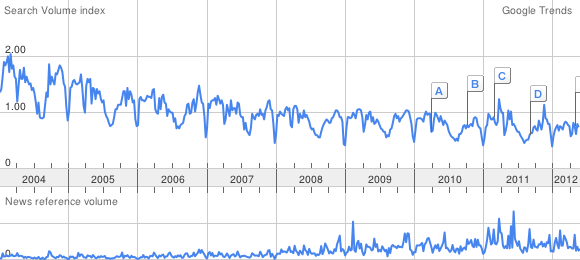
\includegraphics[width=1\linewidth]{google-trends-mobbing.png}}
	\caption{Частота поиска и упоминания в новостях слова mobbing по данным аналитической системы Google Trends.}
	\label{fig:google-trends-mobbing}
\end{figure}

Рассматривая потенциальный вред от разрабатываемой системы, отметим, что все её компоненты являются исключительно программными средствами, а потому физический вред нанести в той же мере, в которой те аппаратные средства, на которых система выполняется. Однако ни в коем случае нельзя оставлять за пределами рассмотрения потенциальный психологический вред. Так, известно наличие в сети Интернет сайтов, таких как 4chan, длительное пребывание на которых, по мнению многих аналитиков\cite{4chan}, может приводить к деформации личности.

К счастью, можно сразу сказать, что система позиционирования транспорта не предполагает взаимодействие между её пользователями, а сама по себе, хоть и использует алгоритмы машинного обучения, не является в достаточной мере интеллектуальной, чтобы наносить психический вред самостоятельно.

Таким образом, имеет смысл рассматривать вред, который может нанести система через ЭВМ. Здесь также можно отметить значительное устаревание имеющихся нормативные документов. Так, основной нормативный документ, описывающий санитарные требования к рабочему месту оператора ЭВМ --- САНПИН 2.2.2/2.4.1340-03\cite{sanpin} уделяет большое внимание вопросу рентгеновского излучения ЭЛТ-мониторов, несмотря на то, что те из них, которые могли сохранить работоспособность до 2012 года, гарантированно относятся к поколению, в котором вся необходимая защита встроена в корпус трубки. С другой стороны, такому явлению, как чтению с экрана, уделено недопустимо мало внимания. Такая характеристика как контрастность вообще не рассматривается, считаются только знаки, как будто они все равноценны. При том, что многие люди действительно не осведомлены о том, что контрастность текста измерять нужно, и делать это в чёрно-белом варианте, в связи с чем недопустим, например, светло-зелёный текст на розовом фоне, хотя эти цвета очень легко различить.

Не уделяется там и внимание такому фактору, давно изучаемому специалистами по интерфейсам, но не специалистами по охране труда, как шрифты. А ведь замечено, что неправильно подобранный шрифт может существенно уменьшить время, которое человек может провести за чтением текста, не устав.

Ещё одним фактором является мерцание и быстрая смена картинки. На это тоже нет никаких нормативов, в связи с чем, зная, что серверная часть разрабатываемой системы будет выводить на экран много текста с большой скоростью, авторам работы остаётся лишь порекомендовать пользователям, во избежание раздражения и покраснения глаз, не злоупотреблять использованием консольного интерфейса сервера, отдавая предпочтение графическому клиенту. Нормировать этот параметр не представляется возможным за отсутствием необходимых норм.

Таким образом, несомненно, можно выделить много потенциально негативных факторов в работе с любым программным продуктом, но те требования, которые были предъявлены 10 лет назад и продолжают предъявляться до сих пор, не соответствуют реальным потребностям повышения юзабилити, не могут быть выполнены и не выполняются в современных условиях, при том, что новые опасные факторы не нормируются или нормируются с большим опозданием.

\chapter{Разработка}

\section{Алгоритм}
В данном подразделе рассматривается алгоритм позиционирования, начиная с того момента, когда данные об уровнях сигнала уже привязаны к точкам на маршруте, а после позиционирования не требуется осуществлять обратное преобразование. Вопрос прямого и обратного преобразования рассмотрен в подпункте \ref{subsubsec:transroute}.

\subsection{Исходные данные}
Исходными данными алгоритма являются, с одной стороны, хранящиеся в базе данных тройки $<CID, RSSI, Dist>$ (CID --- уникальный идентификатор базовой станции, RSSI --- уровень принятого сигнала от неё в точке с координатой Dist), которые были измерены ранее, и значение Dist для которых посчитано на основе данных спутниковой навигации, а с другой --- пары $<CID, RSSI>$ измеренные устройством, координаты которого требуется найти.

\begin{figure}[h]
	\center{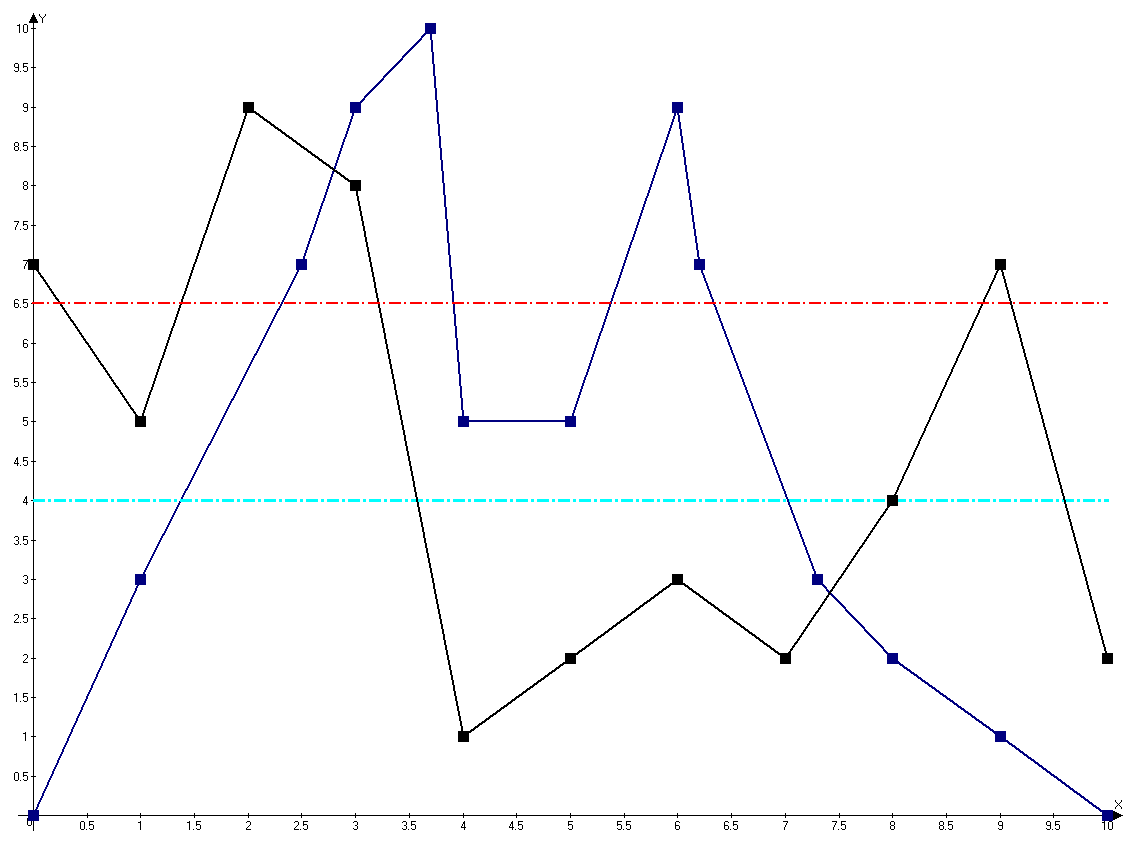
\includegraphics[width=1\linewidth]{MadMax-input.png}}
	\caption{Эскиз возможных входных данных для алгоритма позиционирования. Вертикальная ось --- уровень сигнала, горизонтальная --- координата. Штрихпунктирными линиями обозначены уровни фактически принятых сигналов от двух базовых станций (поскольку их координаты неизвестны, изображены на всём протяжении маршрута). Точки, соединённые сплошными отрезками --- хранящиеся в базе данных замеры RSSI этих станций с известными координатами.}
	\label{fig:madmax-input}
\end{figure}

Эскиз возможного вида таких данных показан на рис. \ref{fig:madmax-input}. Хранящиеся в базе данных замеры соединены прямыми линиями только для того, чтобы не путать замеры сигналов от разных станций на рисунке, реально хранятся только точки. Из базы данных осуществляется выборка тех замеров, CID которых соответствует CID фактически принятых сигналов.

\subsection{Интерполяция}
Для того, чтобы перейти от дискретной оси расстояния к непрерывной, используется интерполяция. Данные о каждой из рассматриваемых базовых станций интерполируются многочленами с помощью линейной регрессии. Из переменной $Dist$ создаётся набор $<1, Dist, Dist^2, Dist^3, ... Dist^n>$. Этот набор вместе со значениями RSSI составляет систему уравнений, решаемую методом нормальных уравнений. Результатом являются коэффициенты многочлена, оптимизированные по методу наименьших квадратов.

Эскиз этого процесса изображён на рис. \ref{fig:madmax-interpol}.
\begin{figure}[H]
	\center{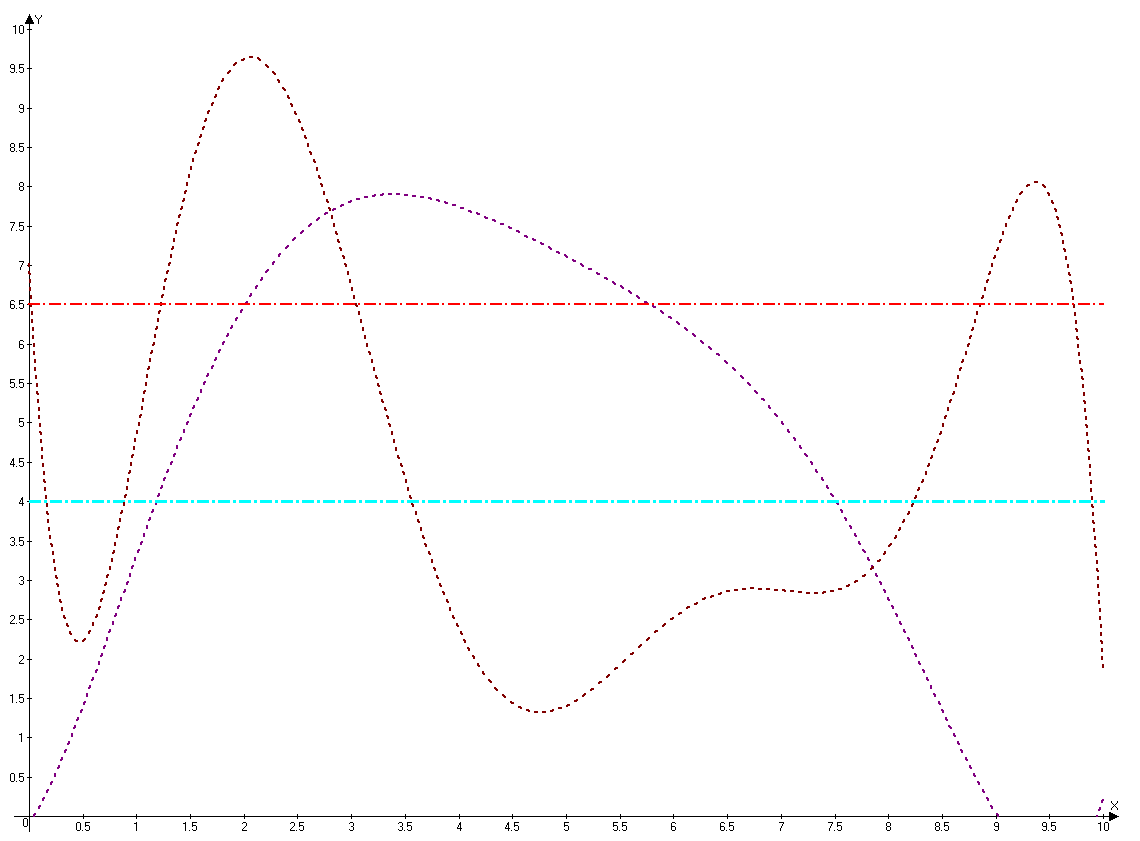
\includegraphics[width=1\linewidth]{MadMax-interpol.png}}
	\caption{Эскиз возможной интерполяции в ходе алгоритма позиционирования. Вертикальная ось --- уровень сигнала, горизонтальная --- координата. Штрихпунктирными линиями обозначены уровни фактически принятых сигналов от двух базовых станций (поскольку их координаты неизвестны, изображены на всём протяжении маршрута), штриховыми --- функции, интерполирующие имеющиеся в базе данных замеры.}
	\label{fig:madmax-interpol}
\end{figure}

\subsection{Вычисление псевдоплотности вероятности}

Одним из ключевых достижений данной работы является введение и применение для позиционирования функции псевдоплотности вероятности.

Определим функцию псевдоплотности вероятности как функцию двух переменных $P(f(x), y)$, где $y$ --- фактически измеренное значение RSSI в некоторой неизвестной точке, а $f(x)$ --- значение интерполяционного многочлена в известной точке $x$, удовлетворяющую следующим условиям:
\begin{enumerate}
	\item
		$\forall_{f(x), y}P(f(x), y)\in(0,1]$
	\item
		$\forall_{f(x), y}f(x) = y\Leftrightarrow{}P(f(x),y) = 1$
	\item
		$\lim\limits_{|f(x)-y|\to\infty}P(f(x),y) = 0$
\end{enumerate}

Функция, удовлетворяющая данным критериям, будет обладать следующим свойством: в любой точке маршрута, чем более фактический замер похож на значением многочлена в данной точке, тем ближе эта функция к 1, а чем дальше --- к 0. Этим свойством данная функция похожа на Байесовское понимание вероятности, а потому названа псевдоплотностью вероятности. Более того, также аналогично Байесовской вероятности, умножение двух таких функций, вычисленных для разных базовых станций, позволяет одновременно сравнивать похожесть по двум параметрам. За счёт того, что операцией, связывающей две псевдоплотности вероятности, является не сложение, как в функции расстояния Махаланобиса (пункт \ref{subsec:mahalanobis} на странице \pageref{subsec:mahalanobis}), а умножение, как в Байесовском классификаторе (пункт \ref{subsec:bayes} на странице \pageref{subsec:bayes}), все выбросы, если только не случится так, что в результате флуктуаций сигнал сразу от нескольких станций станет напоминать другую точку, взаимно уничтожаются.

\begin{figure}[H]
	\center{
		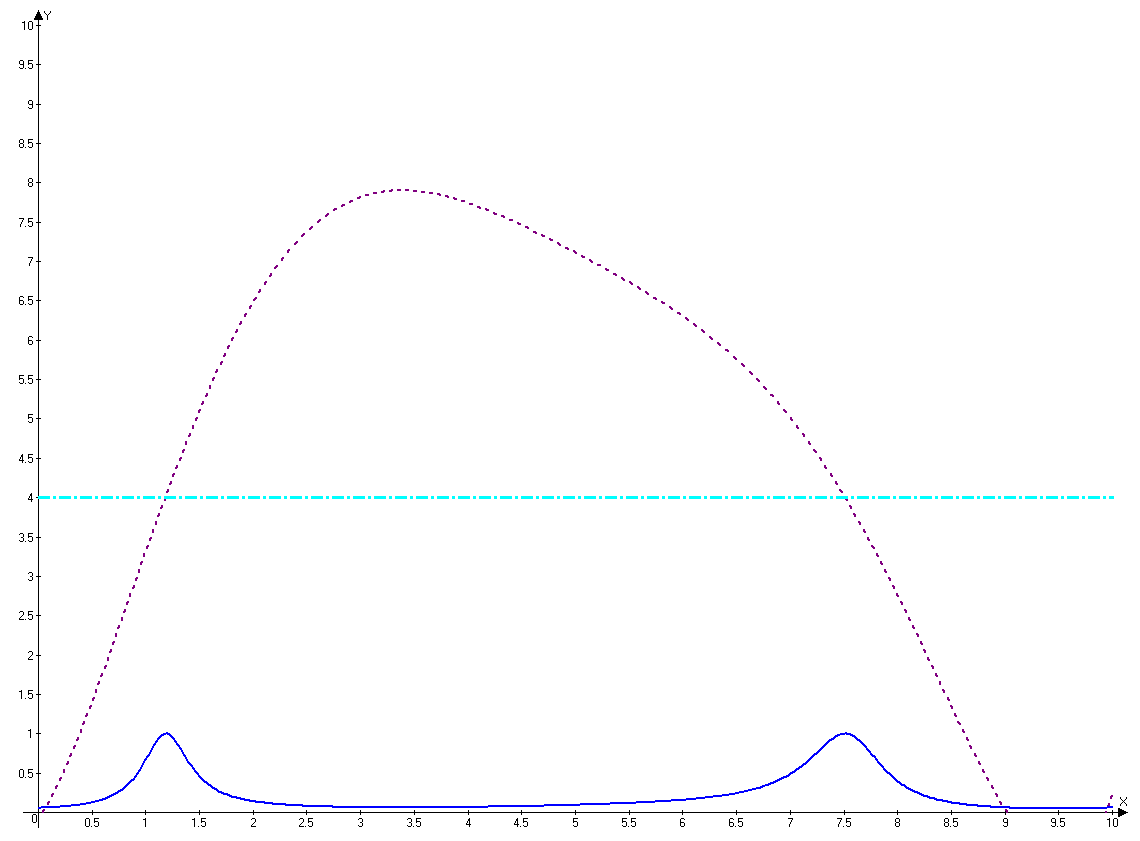
\includegraphics[width=0.7\linewidth]{MadMax-metr-1.png}
		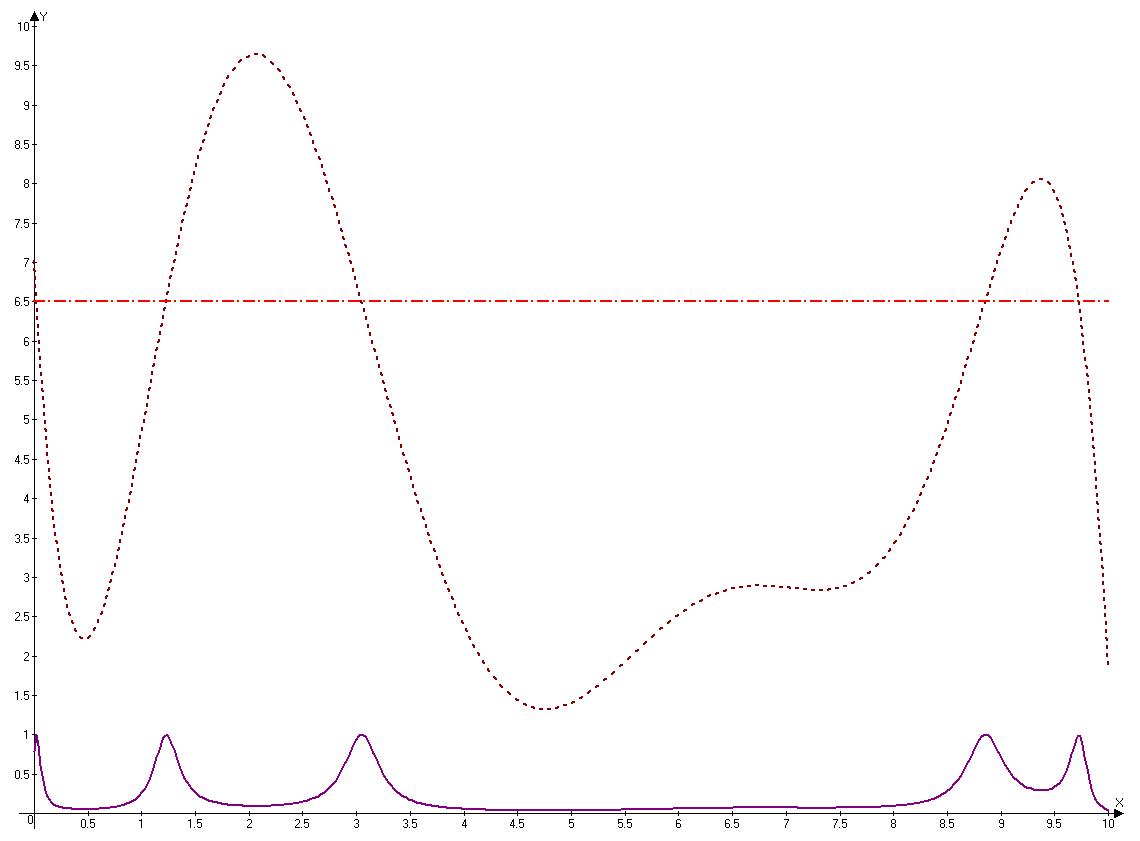
\includegraphics[width=0.7\linewidth]{MadMax-metr-2.png}
	}
	\caption{Эскиз процесса расчёта псевдоплотности вероятности для двух базовых станций. Горизонтальная ось --- расстояние, вертикальная --- RSSI и значение псевдоплотности (не в масштабе). Штрихпунктирная линия --- фактически измеренные значения RSSI, штриховая --- интерполяционный многочлен, сплошная --- значение псевдоплотности.}
	\label{fig:pseudop-draft}
\end{figure}

Отличает такую функцию от настоящей плотности вероятности следующее:
\begin{enumerate}
	\item
		Она может точно достигать значения 1, а не только приближаться к нему;
	\item
		Не требуется, а потому не гарантируется то, что интеграл этой функции по всей области определения равен 1;
	\item
		Даже если нормировать интеграл этой функции на 1, не гарантируется, что интеграл по некоторому участку действительно в точности равен частотной вероятности нахождения там устройства, хотя в Байесовском понимании она отражает степень уверенности в том, что устройство именно там.
\end{enumerate}

Вычисление истинной плотности вероятности не требуется, потому что для работы алгоритма её не нужно интегрировать, а только умножать и искать аргумент максимального значения. А в отношении этих свойств, данная функция сохраняет свойства, присущие плотности вероятности.

Отказ от возможности интегрирования, с другой стороны, позволяет ограничиться очень простым видом функции псевдоплотности вероятности, таким как \ref{eq:pseudop}.
\begin{equation}
	P(f(x), y) = \frac{1}{1+(f(x)-y)^2}
	\label{eq:pseudop}
\end{equation}

Эскиз процесса вычисления псевдоплотности вероятности показан на рис. \ref{fig:pseudop-draft}.

\subsection{Вычисление ответа}

\begin{figure}[H]
	\center{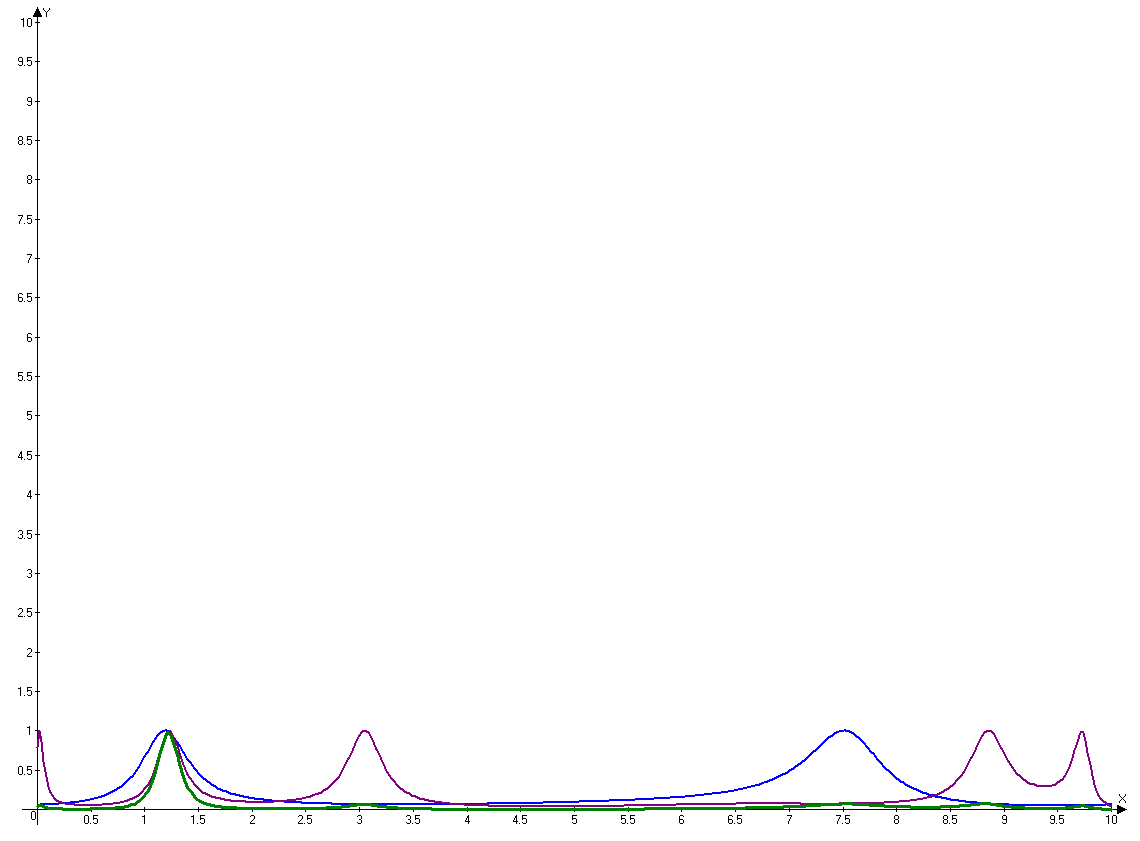
\includegraphics[width=1\linewidth]{MadMax-metr-common.png}}
	\caption{Эскиз произведения функций псевдоплотности для нескольких базовых станций. Горизонтальная ось --- точки на маршруте, вертикальная --- значения псевдоплотности. Результирующая псевдоплотность имеет всего один хорошо выраженный глобальный максимум между координатами 1 и 1,5.}
	\label{fig:total-pseudop-draft}
\end{figure}

После расчёта значений псевдоплотности вероятности для каждой базовой станции, процесс позиционирования сводится к их перемножению и поиску аргумента глобального максимума. Эскиз этого процесса показан на рис. \ref{fig:total-pseudop-draft}.

\section{Мобильное приложение}
Для ОС Android, выполняющейся на устройстве, оборудованном модулями GPS и GSM, а также предоставляющем доступ в интернет, требуется написать приложение, получающее данные об RSSI видимых базовых станций и своём местоположении, после чего передающее их на сервер.

\subsection{Протокол передачи данных}
Собранные данные передаются по протоколу UDP на сервер, будучи записанными в формате JSON в сообщения следующего вида:


\lstset{language=Python}
\begin{lstlisting}
{
	"GSM":{
		"cellcount":2, 
		"cells":[
				{
					"CID":11531, 
					"Psc":-1,
					"RSSI":26,
					"type":"EDGE"
				}, 
				{
					"CID":32779,
					"Psc":-1,
					"RSSI":22,
					"type":"EDGE"
				}
			]
		},
	"GPS": {
			"lng":37.64814019203186,
			"ltd":55.75437605381012,
			"acc":24.0
		}
}
\end{lstlisting}

Значения содержимого полей описаны в таблице \ref{tab:json-raw-format}.
\begin{table}
	\caption{\label{tab:json-raw-format}Значения полей пакета в формате JSON, передаваемого от мобильного устройства на сервер.}
	\begin{center}
		\begin{tabular}{|p{0.2\linewidth}|p{0.2\linewidth}|p{0.5\linewidth}|}
			\hline
			Поле & Тип & Значение \\
			\hline
			GSM & Объект & Набор данных о видимых базовых станций \\
			\hline
			cellcount & Число & Количество станций, передаваемых в данном пакете \\
			\hline
			cells & Массив & Набор объектов, каждый из которых соответствует одной базовой станции \\
			\hline
			CID & Число & Уникальный идентификатор базовой станции, 2 байта \\
			\hline
			Psc & Число & Зарезервировано для сетей 3G \\
			\hline
			RSSI & Число & Уровень принятого сигнала в asu\\
			\hline
			type & Строка & Тип соединения. Возможные значения: <<GPRS>>, <<EDGE>>, <<UMTS>>, <<UNKNOWN>> \\
			\hline
			GPS & Объект & Набор данных спутниковой навигации \\
			\hline
			lng & Число & Долгота в градусах \\
			\hline
			ltd & Число & Широта в градусах \\
			\hline
			acc & Число & Погрешность позиционирования в метрах \\
			\hline
		\end{tabular}
	\end{center}
\end{table}

\subsection{Интерфейсы}

Особенностью программирования под Android SDK является тот факт, что в программе нет аналога функции или метода Main из многих популярных языков программирования. Вся программа состоит из обработчиков различных событий, происходящих в графическом интерфейсе или внутри ОС Android. Запустить код, не зависящий от обработчиков, можно только создав отдельный поток во время обработки одного из событий в главном.

В связи с этим, приложение можно полностью описать через его взаимодействие с иными компонентами.

\subsubsection{Графический интерфейс}
\begin{figure}[h]
	\center{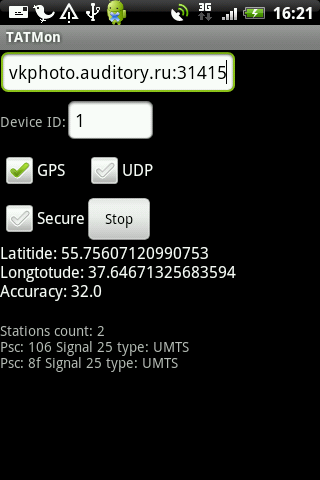
\includegraphics[width=0.5\linewidth]{TATMon-android.png}}
	\caption{Графический интерфейс написанного мобильного приложения, запущенного на телефоне HTC Hero под управлением Android 2.2.}
	\label{fig:tatmon-android}
\end{figure}
Графический интерфейс приложения изображён на рис. \ref{fig:tatmon-android}.
По нажатию кнопки <<Start>>/<<Stop>> начинается или приостанавливается работа фонового потока, обеспечивающего сбор и передачу данных. Этому потоку передаётся адрес и порт, по которому нужно посылать данные, значение флага GPS, определяющего, надо ли передавать данные спутникового позиционирования, или же только уровни сигнала. При неустановленном флаге UDP, фоновый поток не передаёт данные в сеть, а только возвращает их потоку графического интерфейса, который при наступлении такого события как приход сообщения о фонового, обновляет отображаемый список.

Поле Device ID и флаг Secure в описываемой версии не используются.

\subsubsection{Данные об уровнях сигнала}
Информацию об уровнях сигналов видимых базовых станций предоставляется объект класса TelephonyManager, который инстанциируется операционной системой в главном потоке. Информацию он предоставляет через синхронный вызов функции, возвращающей ответ. В связи с этим, обработка этих данных ведётся в фоновом потоке.

\subsubsection{Данные спутниковой навигации}
Данные же GPS поступают асинхронно. При включённом модуле GPS операционная система сама отслеживает факт измерения координат, и создаёт событие обновления, которое можно обработать. Эта обработка осуществляется в главном потоке, после чего её результаты передаются фоновому.

\subsubsection{Взаимодействие с сетью}
Передача данных через UDP осуществляется синхронным вызовом функции, а потому вместе с обработкой данных об уровнях сигнала вынесена в фоновый поток.

\section{Серверная часть}
Сервер, в целом, осуществляет две задачи: приём и обработка поступающих данных и передача результатов работы клиенту. Разница между этими процессами заключается в том, что приходящие по UDP данные обрабатываются синхронно, а передача клиенту по TCP --- асинхронно. В связи с этим, сервер работает в два потока, передача данных между которыми осуществляется через библиотечный класс Queue. Схема этого процесса изображена на рис. \ref{fig:server-threads}.

\begin{figure}[h]
	\center{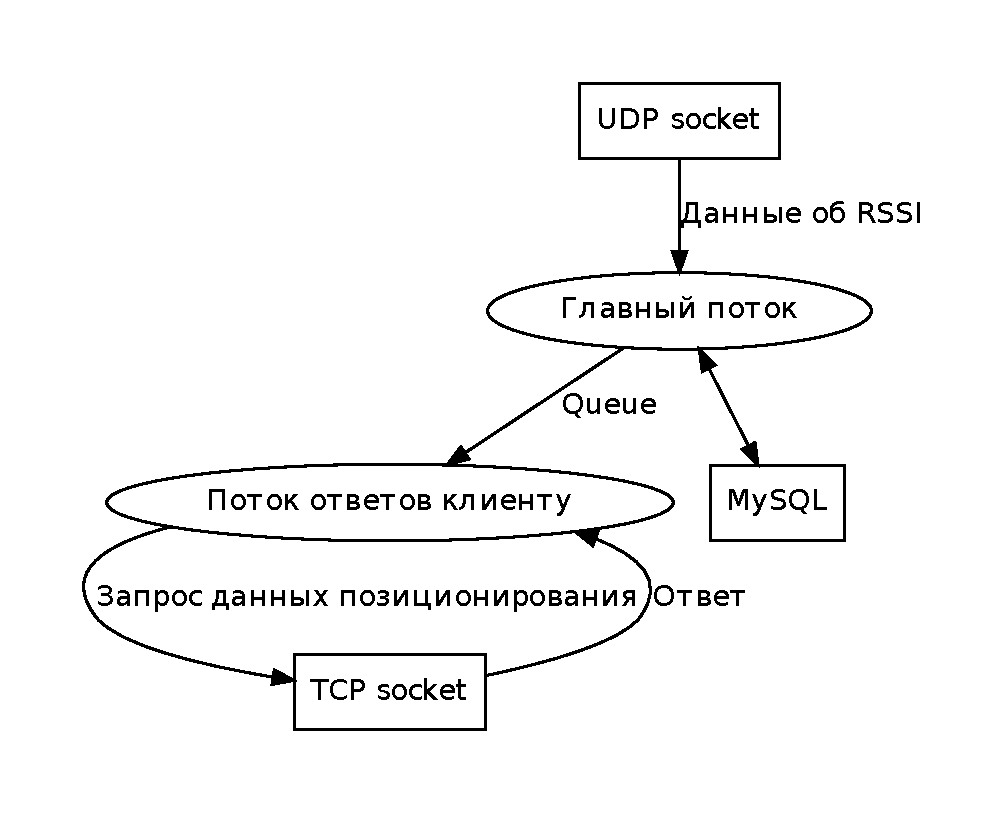
\includegraphics[width=1\linewidth]{server-threads.pdf}}
	\caption{Взаимодействие между потоками сервера (эллипсы) и внешними интерфейсами (прямоугольники).}
	\label{fig:server-threads}
\end{figure}

Сервер может работать в двух режимах --- сбор данных и тестирование позиционирования. Часть классов и модулей является общей для обоих режимов, часть --- специфичной для позиционирования. Начнём, поэтому, с описания режима сбора данных, в рамках описания которого опишем и общие классы.

\subsection{Режим сбора данных}
\begin{figure}[h]
	\center{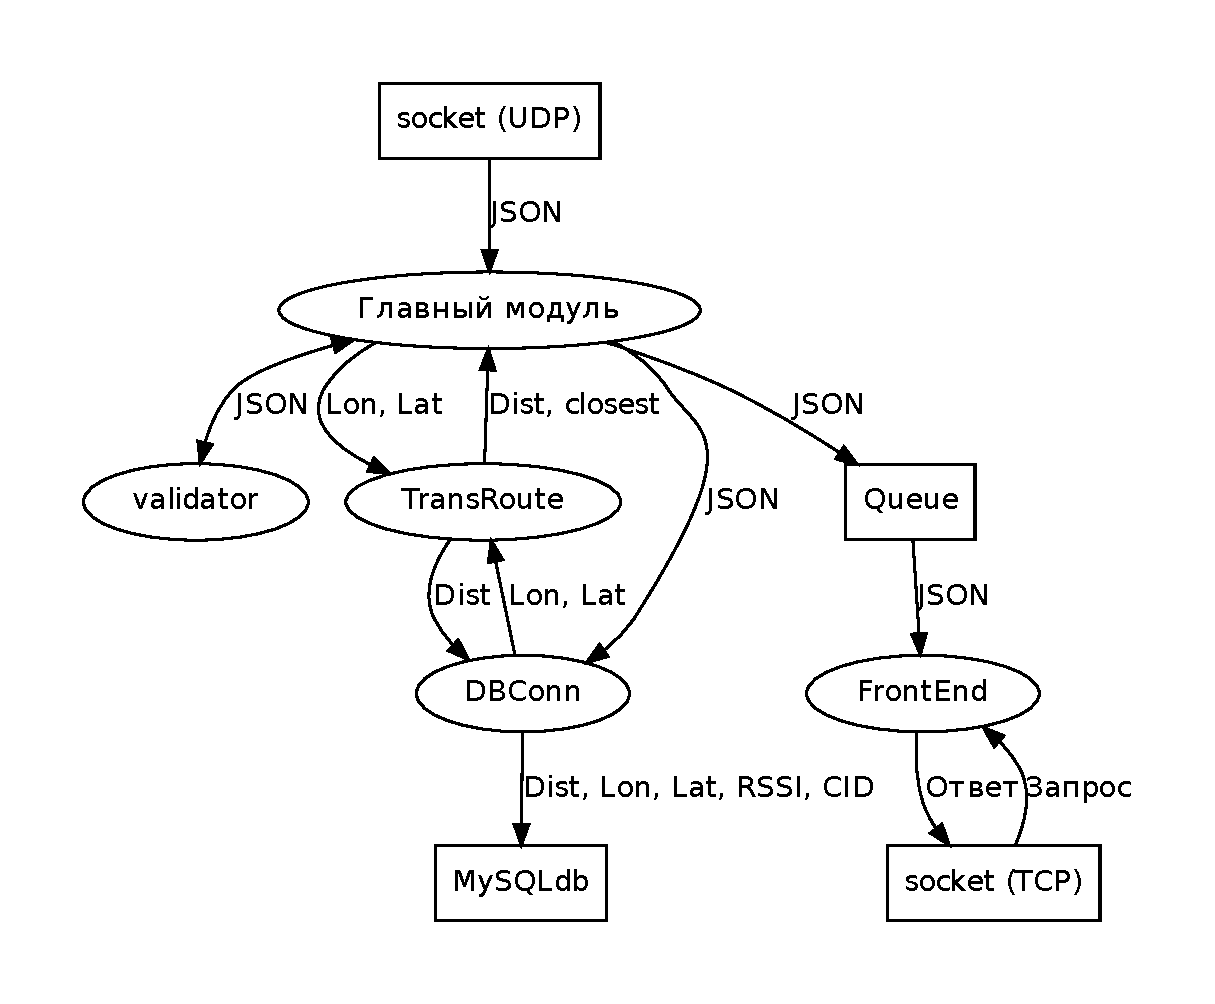
\includegraphics[width=1\linewidth]{server-collect-dataflow.pdf}}
	\caption{Потоки данных между классами сервера (эллипсы) и внешними интерфейсами (прямоугольники) в режиме сбора данных.}
	\label{fig:server-collect-dataflow}
\end{figure}
Общая схема направлений потоков данных в режиме сбора данных изображена на рис. \ref{fig:server-collect-dataflow}. Не отображено преобразование данных в формате JSON во внутренне представление Python, но поскольку и прямое, и обратное преобразование осуществляются каждое одной функцией, их в описании потоков опускаем. Рассмотрим теперь подробнее каждый из классов и модулей, участвующих в обработке данных.

\subsubsection{Проверка входящих данных}
Модуль {\bf validator} содержит единственную функцию с таким же названием, осуществляющую проверку входящих данных на наличие и корректные значения всех полей, описанных в \ref{tab:json-raw-format}. В случае, если находится несоответствие, функция возвращает специальное значение None, получение которого обрабатывается, в противном случае --- переданный объект.

\subsubsection{Преобразование координат}
\label{subsubsec:transroute}
Класс {\bf TransRoute} осуществляет три операции: преобразование пары широта/долгота в расстояние от начала маршрута, обратно --- расстояние в широту и долготу, а также находит точку на маршруте, ближайшую к переданной.

В прототипе системы была реализована обработка единственного маршрута, представляющего собой прямую линию с известными координатами начала и конца. Нетривиальной в таком случае является только одна задача: поиск точки на маршруте, ближайшей к данной. Необходимость её решения вызвана тем, что GPS сам обладает некоторой погрешностью, и может возвращать координаты не строго на маршруте, а немного сбоку от него, поэтому сначала полученную точку надо найти её проекцию на маршрут.

Координаты начала и конца маршрута передаются в конструктор класса, сам класс имеет следующие методы:

\begin{itemize}
	\item
		{\bf closest} --- принимает описание широты и долготы точки в формате JSON, возвращает кортеж из двух координат её проекции на маршрут;
	\item
		{\bf point\_to\_dist} --- принимает описание широты и долготы точки в формате JSON, возвращает число --- расстояние от начала маршрута до проекции переданной точки на него. Расстояние имеет знак, если выйти за границу маршрута со стороны начала, будет также корректным расстоянием по модулю, но отрицательным;
	\item
		{\bf dist\_to\_longlat} --- принимает расстояние от начала маршрута до искомой точки, возвращает её географические координаты.
\end{itemize}

\subsubsection{Взаимодействие с базой данных}
Все запросы к базе данных осуществляются через класс {\bf DBConn}. Подробное описание базы данных находится в подразделе \ref{sec:server-db}, а здесь дано общее описание осуществляемых запросов:
\begin{itemize}
	\item
		{\bf save\_netdata} --- принимает объект JSON с данными о GPS и RSSI, записывает их в базу данных как в виде географических координат, так и в виде точек на маршруте; для преобразования использует класс TransRoute;
	\item
		{\bf avg\_rssi} --- принимает CellID, возвращает среднее значение RSSI по всем точкам;
	\item
		{\bf all\_cells} --- возвращает список из всех CellID, данные о которых имеются в базе;
	\item
		{\bf samples\_by\_sell} --- принимает CellID, возвращает все результаты замеров для неё.
\end{itemize}

\subsubsection{Взаимодействие с клиентами}
\label{subsubsec:server-collect-frontend}
Класс {\bf{}FrontEnd} наследует библиотечный класс {\bf{}threading.Thread} и перегружает единственный метод {\bf{}run}, выполняющийся в отдельном потоке. Метода run, будучи запущенным, открывает сокет для входящих соединений от клиентов, после чего в бесконечном цикле ждёт их. После установки соединения, во вложенном бесконечном цикле пытается считать сообщение из очереди, идущей от главного потока, и если это удалось, посылает его в сокет. При обрыве соединения вложенный бесконечный цикл завершается с исключением, которое обрабатывается внешним, после чего последний снова ожидает соединений.

Передача данных начинается сразу по мере установки соединения клиентом, без ожидание запросов с его стороны. Передаются данные в формате JSON следующего вида:
\begin{lstlisting}
{
	"GPSerrm": 5.8398814870603832,
	"Route": {
		"lng": 37.647922706087265,
		"dstm": 260.0450561256485,
		"dst": 0.0023370777009036913,
		"ltd": 55.754401640921643
	}, 
	"GPSerr": 5.2484200248492898e-05, 
	"GPS": {
		"lng": 55.75437605381012,
		"ltd": 37.647968530654907
		}
}
\end{lstlisting}

Значения полей описаны в таблице \ref{tab:json-collect-format}.

\begin{table}
	\caption{\label{tab:json-collect-format}Значения полей пакета в формате JSON, передаваемого от сервера в режиме сбора данных клиентам.}
	\begin{center}
		\begin{tabular}{|p{0.2\linewidth}|p{0.2\linewidth}|p{0.5\linewidth}|}
			\hline
			Поле & Тип & Значение \\
			\hline
			GPSerrm & Число & Расстояние между точкой и её проекцией на маршрут в метрах \\
			\hline
			Route & Объект & Информация о точке на маршруте \\
			\hline
			lng & Число & Долгота в градусах \\
			\hline
			ltd & Число & Широта в градусах \\
			\hline
			dst & Число & Расстояние от начала маршрута в градусах \\
			\hline
			dstm & Число & Расстояние от начала маршрута в метрах \\
			\hline
			GPSerr & Число & Расстояние между точкой и её проекцией на маршрут в градусах \\
			\hline
		\end{tabular}
	\end{center}
\end{table}

\subsubsection{Главный модуль}
\label{subsubsec:collect-data-main}
Алгоритм работы главного модуля в режиме сбора данных состоит из инициализации всех классов, открытия UDP-сокета для входящих датаграмм от мобильных устройств и перехода в следующий бесконечный цикл:
\begin{enumerate}
	\item
		Принятие сообщения;
	\item
		Проверка сообщения модулем validate;
	\item
		Запись сообщения в базу данных модулем DBConn;
	\item
		Вычисление проекции принятой точки на маршрут, её расстояния от начала маршрута, расстояния между исходной точкой и её проекцией;
	\item
		Запись посчитанных значений в формат JSON и отправка в очередь потока FrontEnd.
\end{enumerate}

\subsection{Режим позиционирования}
Режим позиционирования отличается от режима сбора данных тем, что реакцией на приход сообщения от мобильного устройства является не помещение этой информации в базу данных, а позиционирование на основе собранных данных, проверка качества работы на основе пришедших данных спутникового позиционирования и отправка этих данных клиенту. Соответственно, в архитектуру добавляются классы, обеспечивающие процесс позиционирования. Общий вид потоков данных в режиме позиционирования изображён на рис. \ref{fig:server-perform-dataflow}.

\begin{figure}[h]
	\center{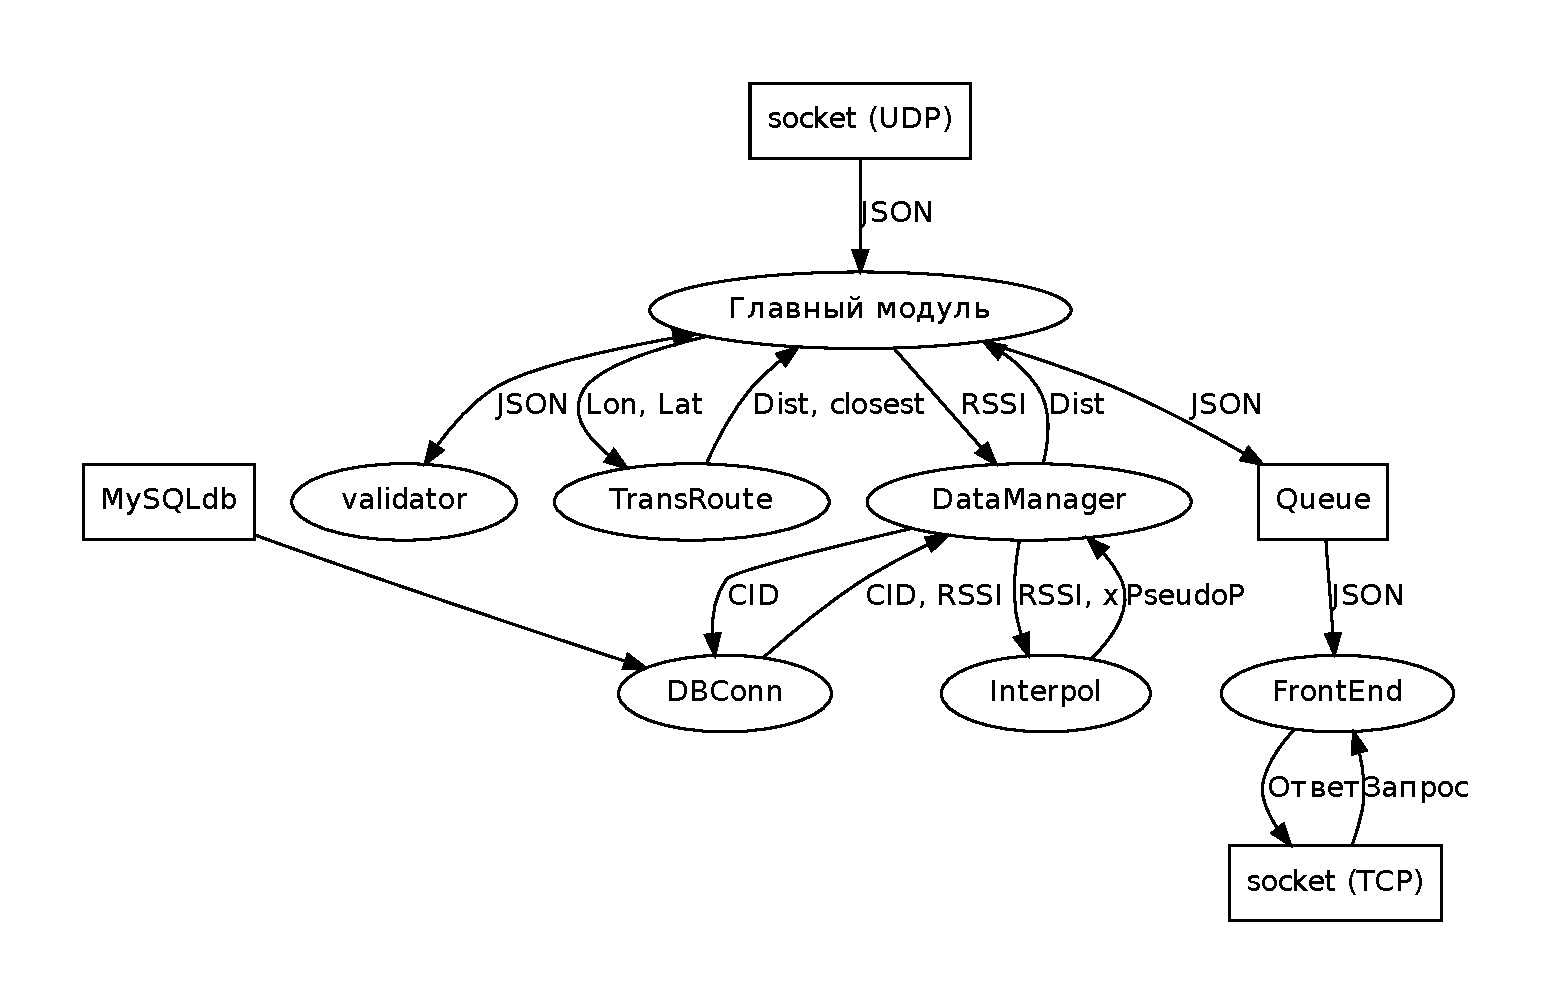
\includegraphics[width=1\linewidth]{server-perform-dataflow.pdf}}
	\caption{Потоки данных между классами сервера (эллипсы) и внешними интерфейсами (прямоугольники) в режиме позиционирования.}
	\label{fig:server-perform-dataflow}
\end{figure}

\subsubsection{Интерполяция и псевдоплотность}
Класс {\bf{}Interpol} предоставляет набор функций для построения интерполирующего многочлена, вычисления его значений для конкретных точек, а также вычисления псевдоплотности вероятности для данной точки на маршруте и данного уровня сигнала. Один экземпляр данного класса описывает перечисленные сущности для одной базовой станции.

Код этого класса, как реализующего основу разработанного математического метода, приводится целиком:

\lstset{language=Python}
\begin{lstlisting}
#-*- coding: utf8 -*-
import numpy
import numpy.linalg

import sys
class Interpol(object):
	def __init__(self, order=10):
		self.order = order
		self.theta = [0]*(self.order+1)

	def create_vars(self, data):
		l = len(data)
		print l
		self.X = numpy.empty([l, self.order+1])
		self.Y = numpy.empty([l, 1])
		try:
			for j in xrange(l):
				for i in xrange(0,self.order+1):
					self.X[j][i] =\
						data[j][0]**i
				self.Y[j][0] = data[j][1]
		except Exception as e:
			print e
			print "i:", i, "j:", j
			print "order:", self.order
			print "data[j]:", data[j]
			print "self.X[j][i]", self.X[j][i]
			print "self.Y[j][0]:", self.Y[j][0]
			sys.exit(0)

	def solve_theta(self):
		self.theta = numpy.transpose(self.X)
		self.theta = numpy.dot(self.theta, self.X)
		self.theta = numpy.linalg.pinv(self.theta)
		self.theta = numpy.dot(self.theta,\
				numpy.transpose(self.X))
		self.theta = numpy.dot(self.theta, self.Y)

	def value(self, x):
		res = 0
		for i in xrange(0, self.order+1):
			res += self.theta[i] * x**i
		return res


	def pseudop(self, x, y):
		return 1.0/(1.0+(self.value(x)-float(y))**2)
\end{lstlisting}

Данный класс использует библиотеку NumPy для быстрых вычислений, предоставляющую интерфейс к ряду математических библиотек, конкретный набор которых зависит от платформы, под GNU/Linux используется GNU Scientific Library\cite{gsl}. Вычисления, даже будучи по своей природе векторными, в случае применения GSL, осуществляются в один поток, однако для данной задачи этого оказалось достаточно.

Конструктор класса {\bf{}\_\_init\_\_} в качестве необязательного аргумента принимает максимальную степень требуемого интерполяционного многочлена, после чего сохраняет её значение в поле order и создаёт массив theta для его коэффициентов.

Два метода должны быть вызваны в обязательном порядке:
\begin{enumerate}
	\item
		{\bf{}create\_vars} --- этот метод в качестве аргумента принимает список data, состоящий из пар $<Dist, RSSI>$ и содержащий все ранее измеренные значения RSSI исследуемой базовой станции в известных точках Dist:
		\begin{equation}
			data = \begin{pmatrix}
				Dist_0 & RSSI_0 \\
				Dist_1 & RSSI_1 \\
				\vdots & \vdots \\
     Dist_{len(data)-1} & RSSI_{len(data)-1}
			\end{pmatrix}
			\label{eq:data-create-vars}
		\end{equation}
		Результатом работы данного метода является запись в поля класса двух массивов: массива self.X, состоящего из векторов $<1, Dist_i, Dist_i^2, ... Dist_i^{order}>$, и массива self.Y, состоящего из значений RSSI, расположенных в том же порядке, что соответствующие им значения $Dist_i$ в массиве self.X:
		\begin{equation}
			self.X = \begin{pmatrix}
				1 & Dist_0 & Dist_0^2 & \cdots & Dist_0^{order} \\
				1 & Dist_1 & Dist_1^2 & \cdots & Dist_1^{order} \\
      \vdots & \vdots & \vdots & \vdots & \vdots \\
				       1 & Dist_{len(data)-1} & Dist_{len(data)-1}^2 & \cdots & Dist_{len(data)-1}^{order}
			\end{pmatrix}
			\label{eq:self-x-create-vars}
		\end{equation}
		\begin{equation}
			self.Y = \begin{pmatrix}
				RSSI_0 \\
				RSSI_1 \\
				\vdots \\
				RSSI_{len(data)-1}
			\end{pmatrix}
			\label{eq:self-y-create-vars}
		\end{equation}
	\item
		{\bf{}solve\_theta} --- результатом вызова этого метода является нахождение коэффициентов интерполяционного многочлена по методу нормальных уравнений и запись их в массив self.theta:
		\begin{equation}
			self.theta = (self.X^\intercal \cdot self.X)^{+} \cdot self.X^\intercal \cdot self.Y
			\label{eq:solve-theta}
		\end{equation}
		Отметим, что в ходе решения используется не обычная инверсия, а нахождение псевдообратной матрицы, что позволяет сохранить работоспособность системы даже в случае, когда система неразрешима в рамках обычного метода нормальных уравнений.
\end{enumerate}

После того, как были вызваны эти методы, становится доступным вызов метода {\bf{}value}, возвращающего значение интерполяционного многочлена в переданной точке, и метода {\bf{}pseudop}, для заданной точки и заданного уровня RSSI возвращающего значение псевдоплотности вероятности.

\subsubsection{Результирующая псевдоплотность и позиционирование}

Класс {\bf{}DataManager} отвечает за хранение коллекции экземпляров класса Interpol, соответствующих различным базовым станциям, и использование их для позиционирования устройств. В прототипе системы приняты следующие соглашения:

\begin{enumerate}
	\item
		Интерполяционные многочлены строятся при инициализации сервера в режиме позиционирования, сразу для всех имеющихся в базе данных CellID;
	\item
		Одновременно сервер работает только в одном из режимов, а потому во время работы в режиме позиционирования, состояние базы данных измениться не может, и перестраивать многочлены гарантированно не потребуется;
	\item
		Весь процесс выборки данных из базы, соответственно, происходит только во время инициализации, после чего в течение всего времени работы сервера интерполяционные многочлены хранятся в оперативной памяти.
\end{enumerate}

С учётом этих соглашений, рассмотрим работу класса DataManager. При вызове конструктора класса создаётся подключение к базе данных через класс DBConn, после чего в обязательном порядке должны быть вызваны следующие методы:

\begin{enumerate}
	\item
		{\bf{}fetch\_cells} --- этот метод передаёт классу DBConn запрос на получение списка всех CellID, имеющихся в базе данных, после чего записывает результат в своё поле self.cells;
	\item
		{\bf{}build\_interpols} --- для каждого из полученных CellID, этот метод передаёт классу DBConn запрос на получение всех результатов измерений, связанных с данной базовой станцией, после чего создаёт объект класса Interpol, у которого вызывает метод create\_vars со списком измерений в качестве аргумента, после чего вызывает метод solve\_theta. Полученный объект, готовый к использованию для вычисления псевдоплотности, помещается в ассоциативный массив self.cellfuncs с CellID в качестве индекса.
\end{enumerate}

После вызова этих методов, становятся доступными следующие:
\begin{itemize}
	\item
		{\bf{}total\_pseudop} --- для заданного списка $<CID, RSSI>$ и заданной точки на маршруте, вычисляет значения псевдоплотности, после чего перемножает их между собой и возвращает результат.
	\item
		{\bf{}position} --- для заданного списка $<CID, RSSI>$ перебирает все возможные значения x и возвращает то, для которого значение общей псевдоплотности было максимальным. Для работы прототипа системы, даже такого простого метода поиска максимума оказалось достаточно, хотя, в случае реализации для промышленного применения, его стоит заменить на более эффективный.
\end{itemize}

\subsubsection{Главный модуль}
\label{subsubsec:server-perform-main}
Алгоритм работы главного модуля в режиме позиционирования схож с алгоритмом в режиме сбора данных (см. подпункт \ref{subsubsec:collect-data-main}), а отличается тем, что в начале работы, среди прочих, инициализируется класс DataManager, а бесконечный цикл состоит из следующих этапов:

\begin{enumerate}
	\item
		Приём данных от мобильного устройства;
	\item
		Валидация принятых данных;
	\item
		Позиционирование по данным GSM с помощью класса DataManager;
	\item
		Перевод координат полученной точки из одного числа --- расстояния от начала маршрута --- в пару широта/долгота;
	\item
		Сравнение полученных данных с данными GPS, также принятыми от мобильного устройства;
	\item
		Отправка всех вычисленных данных в формате JSON в очередь класса FrontEnd.
\end{enumerate}

Клиенту от сервера передаётся сообщение в формате JSON следующего вида:
\begin{lstlisting}
{
    "RouteGPS": {
        "dstd": 0.0033751292307418156, 
        "dstm": 375.73660822935375, 
        "fromtruem": 13.135102486978056, 
        "lng": 55.755307975824707, 
        "ltd": 37.648428777250331
    }, 
    "RouteGSM": {
        "dstm": 336.50000000000193, 
        "lng": 37.648256950398967, 
        "ltd": 55.755000247022828
    }, 
    "TrueGPS": {
        "acc": 8.0, 
        "lng": 55.755250453948975, 
        "ltd": 37.648531794548035
    }
}
\end{lstlisting}

Описание значения полей даны в таблице \ref{tab:json-perform-format}.

\begin{table}
	\caption{\label{tab:json-perform-format}Значения полей пакета в формате JSON, передаваемого от сервера в режиме позиционирования клиентам.}
	\begin{center}
		\begin{tabular}{|p{0.2\linewidth}|p{0.2\linewidth}|p{0.5\linewidth}|}
			\hline
			Поле & Тип & Значение \\
			\hline
			RouteGPS & Объект & Набор данных о проекции истинного положения устройства на маршрут \\
			\hline
			dsts & Число & Расстояние от начала маршрута до проекции положения в градусах \\
			\hline
			dstm & Число & Расстояние от начала маршрута до проекции положения в метрах \\
			\hline
			fromtruem & Число & Расстояние от истинного положения до его проекции на маршрут в метрах \\
			\hline
			lng & Число & Долгота в градусах \\
			\hline
			ltd & Число & Широта в градусах \\
			\hline
		   	RouteGSM & Объект & Набор данных о результатах позиционирования по сигналу GSM \\
			\hline
			TrueGPS & Объект & Набор данных об истинном положении мобильного устройства по данным спутниковой навигации \\
			\hline
			acc & Число & Погрешность GPS в метрах\\
			\hline
		\end{tabular}
	\end{center}
\end{table}

\section{База данных}
\label{sec:server-db}
Необходимость хранить данные об отношении между точками на маршруте и результатами измерений уровней сигнала в них, по определению, говорит о необходимости использования реляционной модели.

В разработанном прототипе системы используется простая база данных, состоящая из двух таблиц, хранящих результаты измерений RSSI в различных точках маршрута для различных базовых станций. Никакие другие другие данные длительного хранения не требуют.

Имеющиеся таблицы объявлены следующим образом:

\lstset{language=SQL}
\begin{lstlisting}
CREATE TABLE IF NOT EXISTS raw_rssi_data (
	Longitude DOUBLE NOT NULL,
	Latitude DOUBLE NOT NULL,
	CellID INT NOT NULL,
	ObservedRSSI INT NOT NULL,
	Observations INT NOT NULL,
	PRIMARY KEY (Longitude, Latitude, CellID, ObservedRSSI),
	INDEX (CellID)
) ENGINE=InnoDB;

CREATE TABLE IF NOT EXISTS route_rssi_data (
	Route INT NOT NULL,
	Distance DOUBLE NOT NULL,
	CellID INT NOT NULL,
	ObservedRSSI INT NOT NULL,
	Observations INT NOT NULL,
	PRIMARY KEY (Route, Distance, CellID, ObservedRSSI),
	INDEX (CellID)
) ENGINE=InnoDB;
\end{lstlisting}

\begin{table}
	\caption{\label{tab:server-db}Значения столбцов в таблицах базы данных сервера}
	\begin{center}
		\begin{tabular}{|p{0.2\linewidth}|p{0.7\linewidth}|}
			\hline
			Столбец & Значение \\
			\hline
			Longitude & Долгота в градусах \\
			\hline
			Latitude & Широта в градусах \\
			\hline
			CellID & Уникальный идентификатор базовой станции, целое число \\
			\hline
			ObservedRSSI & Измеренное значение уровня сигнала от данной базовой станции в данной точке в asu\\
			\hline
			Observations & Количество раз, которое уровень сигнала от данной базовой станции принимал в данной точке данное значение\\
			\hline
			Distance & Расстояние от начала маршрута в градусах \\
			\hline
			Route & Номер маршрута, зарезервировано для дальнейшего развития \\
			\hline
		\end{tabular}
	\end{center}
\end{table}

Значения их столбцов описаны в таблице \ref{tab:server-db}. Видно, что имеющие таблицы дублируют друг друга. Такая архитектура была выбрана в связи с тем, что для работы сервера требуется только данные из таблицы route\_rssi\_data, ассоциация же результатов измерений с их истинным положением, а не его проекцией на маршрут, требуется только для целей сбора и анализа статистики. Таким образом, таблицу raw\_rssi\_data следует считать хранилищем отладочной информации, а реально используемой базой данных --- только route\_rssi\_data.

\subsection{Добавление информации в БД}
Хранение для каждой точки и каждой базовой станции не среднего результата всех замеров, а количества наблюдений для каждого из наблюдавшегося уровня по отдельности, по сути, представляет собой хранение распределения. Это позволяет однозначно восстановить все когда-либо сделанные замеры (что используется для увеличения множества, на котором строятся интерполяционные многочлены), при этом не перегружая базу уникальными идентификаторами для каждого наблюдения.

С другой стороны, это усложняет добавление информации о новом наблюдении в базу. Оно разделяется на два случая:
\begin{enumerate}
	\item
		Если для измеренной тройки $<Distance, CellID, ObservedRSSI>$ в таблице уже имеется строка с точно такими же значениями, требуется увеличить на 1 значение ячейки Observations этой строки;
	\item
		Если же таких значений нет, подобную строку надо добавить в таблицу, установив значение ячейки Observations в 1.
\end{enumerate}

Поскольку MySQL не поддерживает триггеры типа <<INSTEAD OF INSERT>>\cite{triggersyntax}, осуществляет эту операцию сервер по следующему алгоритму:
\begin{enumerate}
	\item
		Начало транзакции;
	\item
		Запрос вида: <<SELECT Longitude, Latitude, CellID, ObservedRSSI FROM\\* raw\_rssi\_data WHERE Longitude = \%4.15f AND Latitude = \%4.15f AND CellID = \%d AND ObservedRSSI = \%d>>;
	\item
		\begin{itemize}
			\item
				Если результат запроса пустой --- запрос вида: <<INSERT INTO\\* raw\_rssi\_data(Longitude, Latitude, CellID, ObservedRSSI, Observations) VALUES (\%4.15f, \%4.15f, \%d, \%d, \%d)>>;
			\item
				Иначе --- запрос вида: <<UPDATE raw\_rssi\_data SET Observations = Observations + 1 WHERE Longitude = \%4.15f AND Latitude = \%4.15f AND CellID = \%d AND ObservedRSSI = \%d>>;
		\end{itemize}
	\item
		Конец транзакции.
\end{enumerate}

\section{Клиентская часть}
Несмотря на то, что основная информация о работе сервера собиралась с помощью текстовых журналов, для контроля его работы в реальном времени был написан графический клиент на языке Python с использованием библиотеки Pygame.

\begin{figure}[h]
	\center{
		\begin{subfigure}[b]{0.7\textwidth}
			\center{
				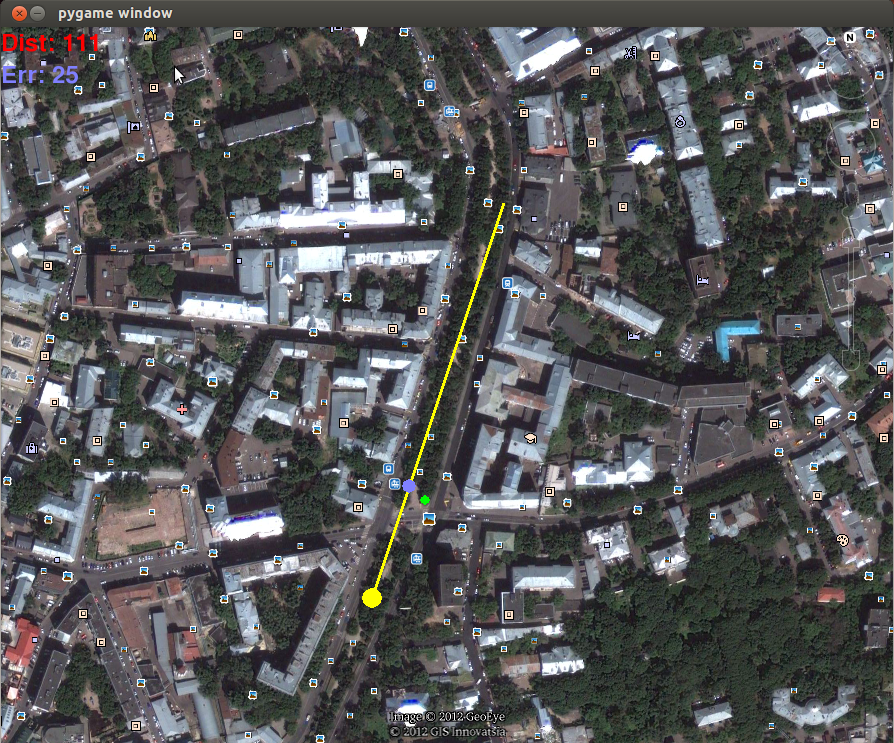
\includegraphics[width=\textwidth]{gfront-gps-mode.png}
				\caption{Сбор данных}
			}
			\label{subfig:gfront-gps-mode}
		\end{subfigure}
	
		\begin{subfigure}[b]{0.7\textwidth}
			\center{
				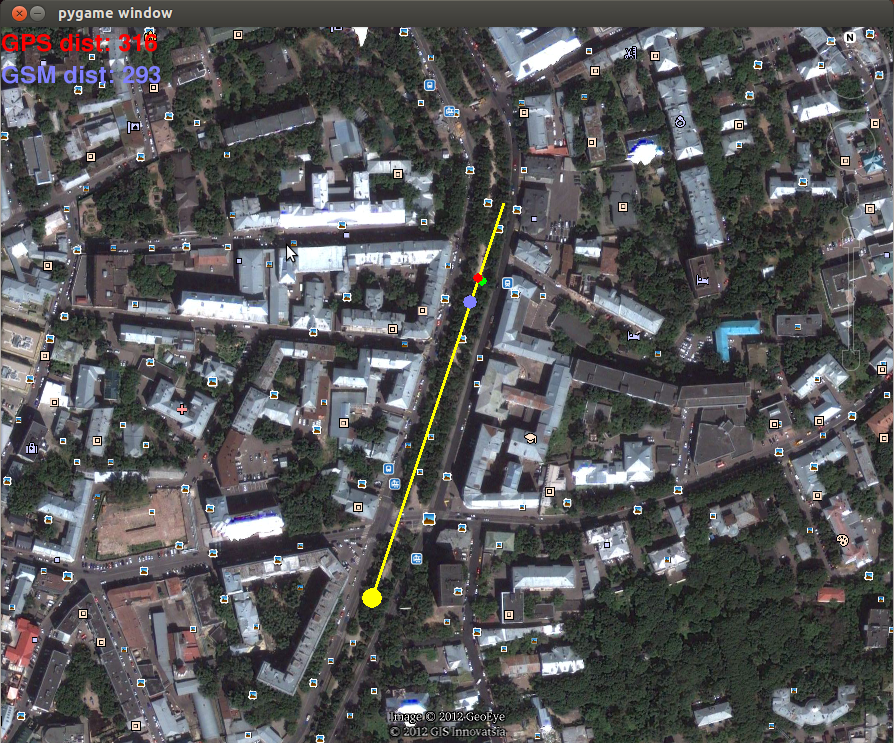
\includegraphics[width=\textwidth]{gfront-gsm-mode.png}
				\caption{Позиционирование}
			}
			\label{subfig:gfront-gsm-mode}
		\end{subfigure}
	}
	\caption{Снимки работы графического клиента в двух возможных режимах. Изображение местности взято из приложения Google Earth\cite{googleearth} на условиях Fair use\cite{enwikifairuse}.}
	\label{fig:gfront}
\end{figure}

Данное приложение отображает на экране вид сверху на местность, где осуществлялось тестирование приложения (снимок взят из приложения Google Earth\cite{googleearth} на условиях Fair use\cite{enwikifairuse}), поверх которого рисует жёлтым цветом линию маршрута, обозначив его начало кругом того же цвета (см. рис. \ref{fig:gfront}).

Приложение, будучи запущенным, открывает соединение с сервером по протоколу TCP и начинает ждать передачи данных. При приходе сообщения в формате JSON, клиент определяет режим работы сервера по содержимому принятого сообщения (см. подпункты \ref{subsubsec:server-collect-frontend} и \ref{subsubsec:server-perform-main}), после чего сам переключается в соответствующий режим (менять режим возможно с каждым новым пакетом, если это потребуется).

\subsection{Режим сбора данных}
В режиме сбора данных (рис. \ref{fig:gfront}\subref{subfig:gfront-gps-mode}) клиент отображает на карте зелёной точкой истинное положение мобильного устройства по данным GPS, а голубой --- её проекцию на маршрут. На экране отображается параметр Dist, означающий расстояние в метрах от начала маршрута до проекции положения мобильного устройства на него, и Err --- расстояние от истинного положения до его проекции на маршрут в метрах.

\subsection{Режим позиционирования}
В режиме позиционирования (рис. \ref{fig:gfront}\subref{subfig:gfront-gsm-mode}) клиент отображает на карте:
\begin{itemize}
	\item
		{\bf{}Зелёная точка} --- истинное положение устройства по данным GPS;
	\item
		{\bf{}Красная точка} --- проекция истинного положения на маршрут;
	\item
		{\bf{}Голубая точка} --- результат позиционирования по данным GSM.
\end{itemize}

Параметры GPS dist и GSM dist означают расстояние от начала маршрута до положения устройства по данным GPS и GSM соответственно.

\chapter{Экспериментальная проверка}

\section{Условия эксперимента}
\begin{itemize}
	\item
		Проверка работы созданного прототипа осуществлялась в мае 2012 года на прямом тестовом участке длиной около 400 метров, проходящем по Покровскому и Яузскому бульварам в Москве (см. рис. \ref{fig:gfront});
	\item
		В качестве мобильного устройства использовался HTC Hero под управлением ОС Android 2.2 (см. рис. \ref{fig:tatmon-android});
	\item
		Сервер был запущен на VPS vkphoto.auditory.ru под управлением дистрибутива Gentoo ОС GNU/Linux версии 2.6.28-vs2.3.0.36.4-gentoo-ws0 с интерпретатором Python версии 2.6.4;
	\item
		Передача данных от мобильного устройства серверу по протоколу UPD осуществлялась через порт 31415;
	\item
		Входящие соединения TCP для передачи данных клиентам сервер принимал через порт 31416.
\end{itemize}

\section{Сбор данных}
Данные собирались в течение часа, по возможности равномерным образом по всей длине маршрута. В ходе эксперимента выяснился факт сравнительно редкого обновления данных GPS под Android, поэтому во время перемещения по маршруту передача данных выключалась до тех пор, пока показания широты и долготы не поменяются, затем включалась заново. Дополнительно осуществлялся контроль правильности обработки данных о местоположении путём визуального сравнения показаний клиентского приложения (см. рис. \ref{fig:gfront}\subref{subfig:gfront-gps-mode}), запущенного на портативном компьютере, подключённым к сети Интернет через общий канал с мобильным устройством, с фактической обстановкой вокруг. Координаты тестового маршрута отражены в таблице \ref{tab:exp-route-begend}. Общая статистика собранных данных отражена в таблице \ref{tab:exp-collect-data}.
\begin{table}
	\caption{\label{tab:exp-route-begend}Координаты крайних точек тестового прямого маршрута.}
	\begin{center}
		\begin{tabular}{|p{0.3\linewidth}|p{0.3\linewidth}|p{0.3\linewidth}|}
			\hline
			Точка & Широта, градусов & Долгота, градусов \\
			\hline
			Начало & 55.752361111111114 & 37.64678333333333 \\
			\hline
			Конец & 55.755430555555556 & 37.64849722222222 \\
			\hline
		\end{tabular}
	\end{center}
\end{table}

\begin{table}
	\caption{\label{tab:exp-collect-data}Статистика по собранным данным во время экспериментальной проверки системы.}
	\begin{center}
		\begin{tabular}{|p{0.8\linewidth}|p{0.1\linewidth}|}
			\hline
			Всего замеров уровней сигнала & 22675 \\
			\hline
			Замеров с различающимися значениями $<CID, Dist, RSSI>$ & 10020 \\
			\hline
			Всего различных базовых станций & 22 \\
			\hline
			Время сбора данных & 1 час \\
			\hline
		\end{tabular}
	\end{center}
\end{table}




\section{Позиционирование}
Рассмотрим трассировку процесса позиционирования, осуществлённого после сбора данных с произвольно выбранным сообщением от мобильного устройства.

\subsection{Входные данные}
Было выбрано следующее сообщение:

\lstset{language=Python}
\begin{lstlisting}
{
	"GSM":{
		"cellcount":6,
		"cells": [
				{
					"CID":41526,
					"Psc":-1,
					"RSSI":21,
					"type":"EDGE"
				},
				{
					"CID":32778,
					"Psc":-1,
					"RSSI":28,
					"type":"EDGE"
				}, 
				{
					"CID":32777,
					"Psc":-1,
					"RSSI":20,
					"type":"EDGE"
				}, 
				{
					"CID":12056,
					"Psc":-1,
					"RSSI":18,
					"type":"EDGE"
				},
				{
					"CID":14296,
					"Psc":-1,
					"RSSI":20,
					"type":"EDGE"
				},
				{
					"CID":32779,
					"Psc":-1,
					"RSSI":15,
					"type":"EDGE"
				}
			]
	}, 
	"GPS": {
		"lng":37.647523283958435,
		"ltd":55.7536518573761,
		"acc":16.0
		}
}
\end{lstlisting}

По данным класса TransRoute, расстояние от начала маршрута до проекции этой точки составляет 165,5 метров.

\subsection{Выборка собранных данных}
На этом этапе для всех имеющихся в массиве cells базовых станций осуществляется выборка ранее измеренных значений из базы данных. Графики этих значений, для каждой станции по отдельности, изображены на рис. \ref{fig:exp-cell-raw}.

\begin{figure}[p]
	\begin{center}
		\begin{subfigure}[b]{1\textwidth}
			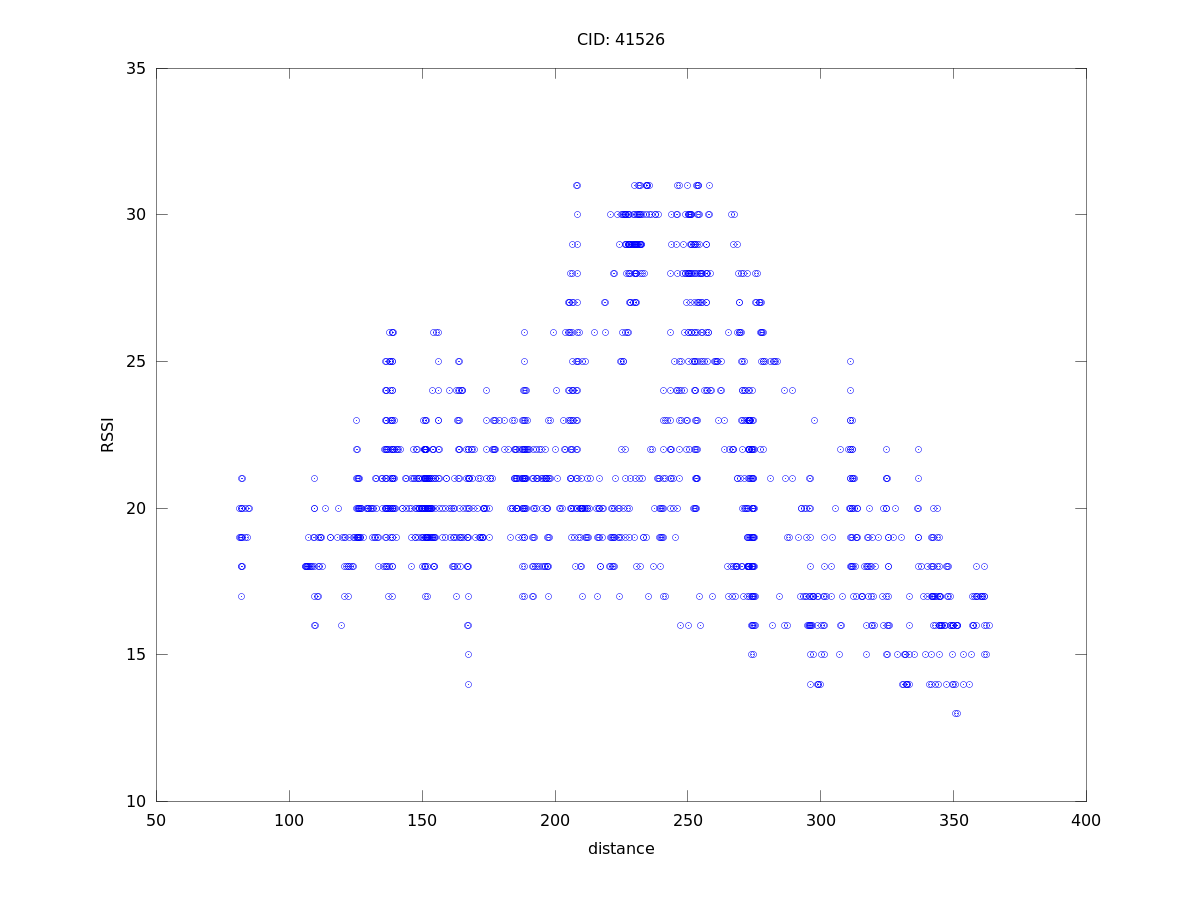
\includegraphics[width=1\textwidth]{cell41526raw.png}
		\end{subfigure}

		\begin{subfigure}[b]{0.45\textwidth}
			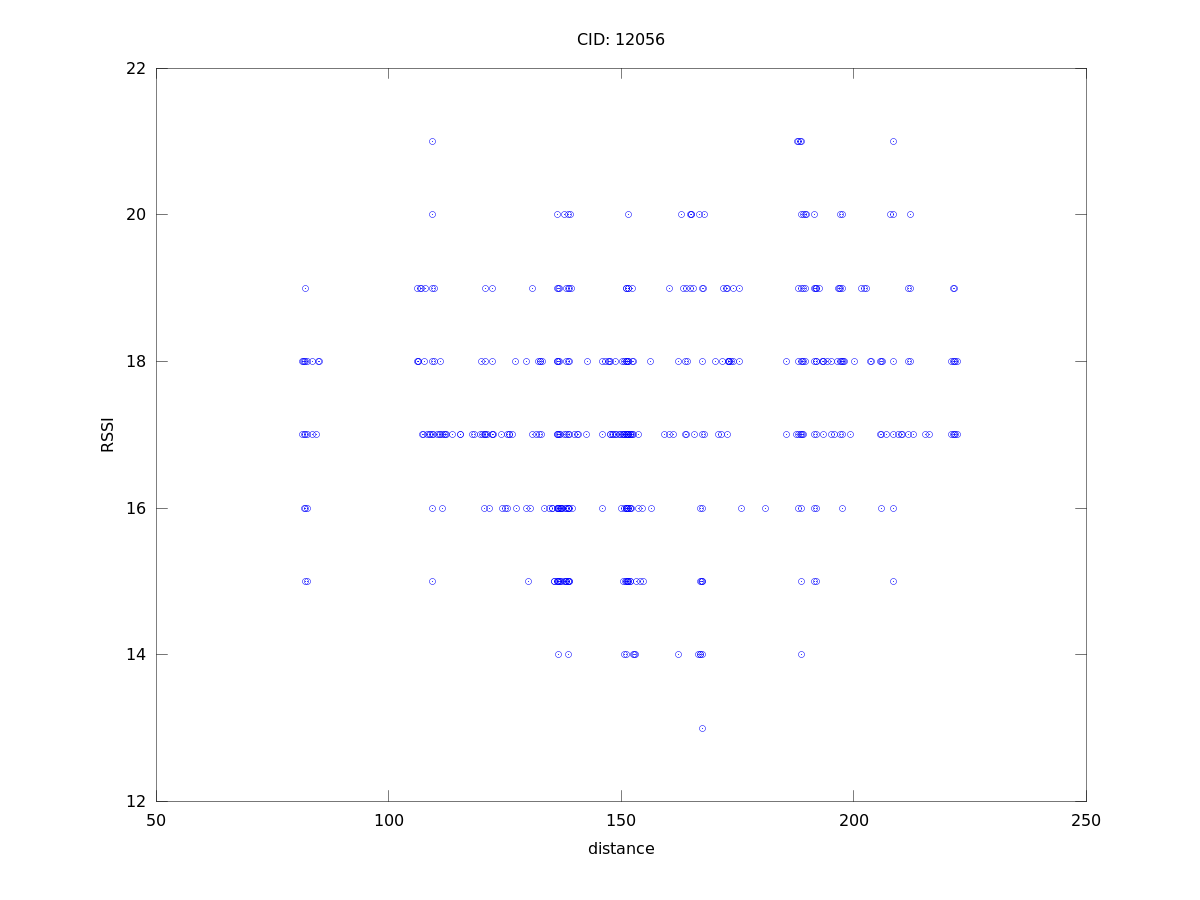
\includegraphics[width=1\textwidth]{cell12056raw.png}
		\end{subfigure}
		\begin{subfigure}[b]{0.45\textwidth}
			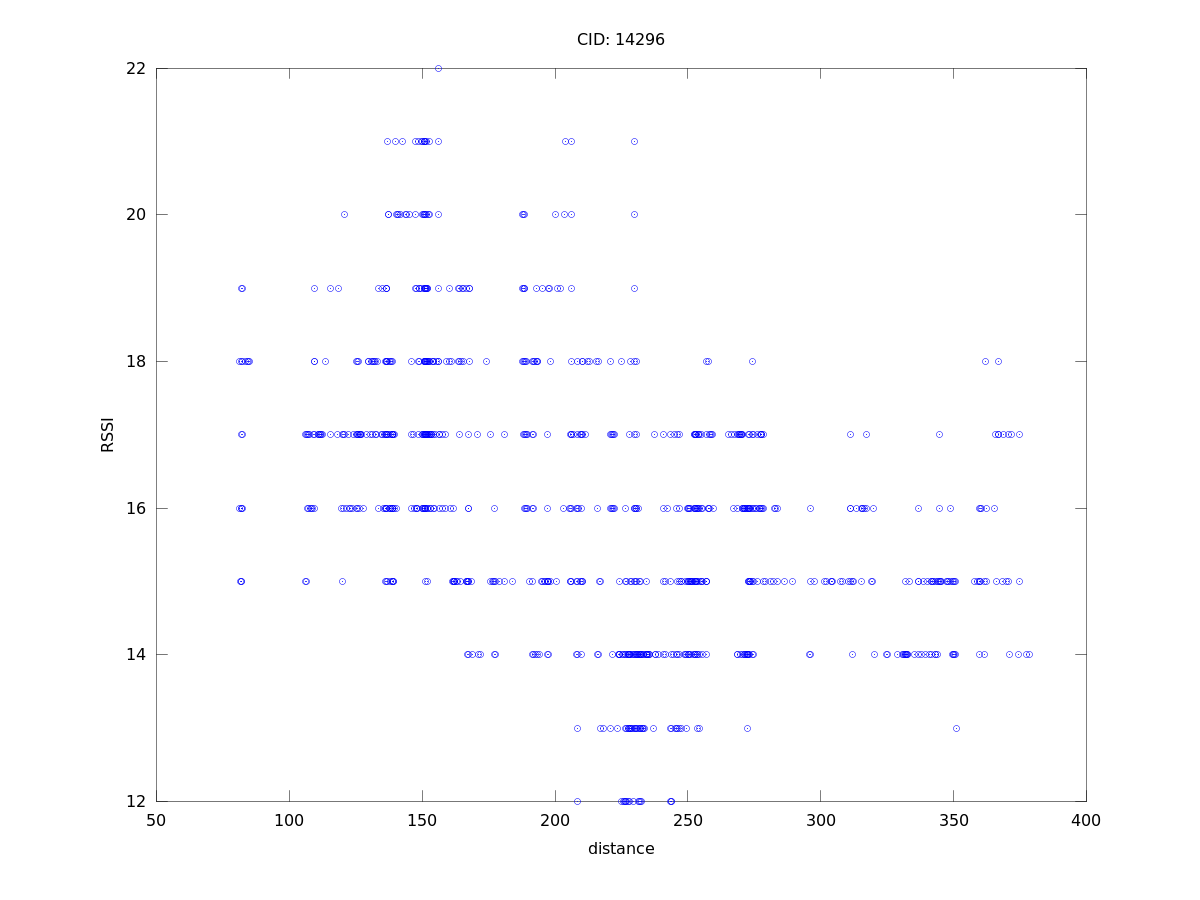
\includegraphics[width=1\textwidth]{cell14296raw.png}
		\end{subfigure}

		\begin{subfigure}[b]{0.3\textwidth}
			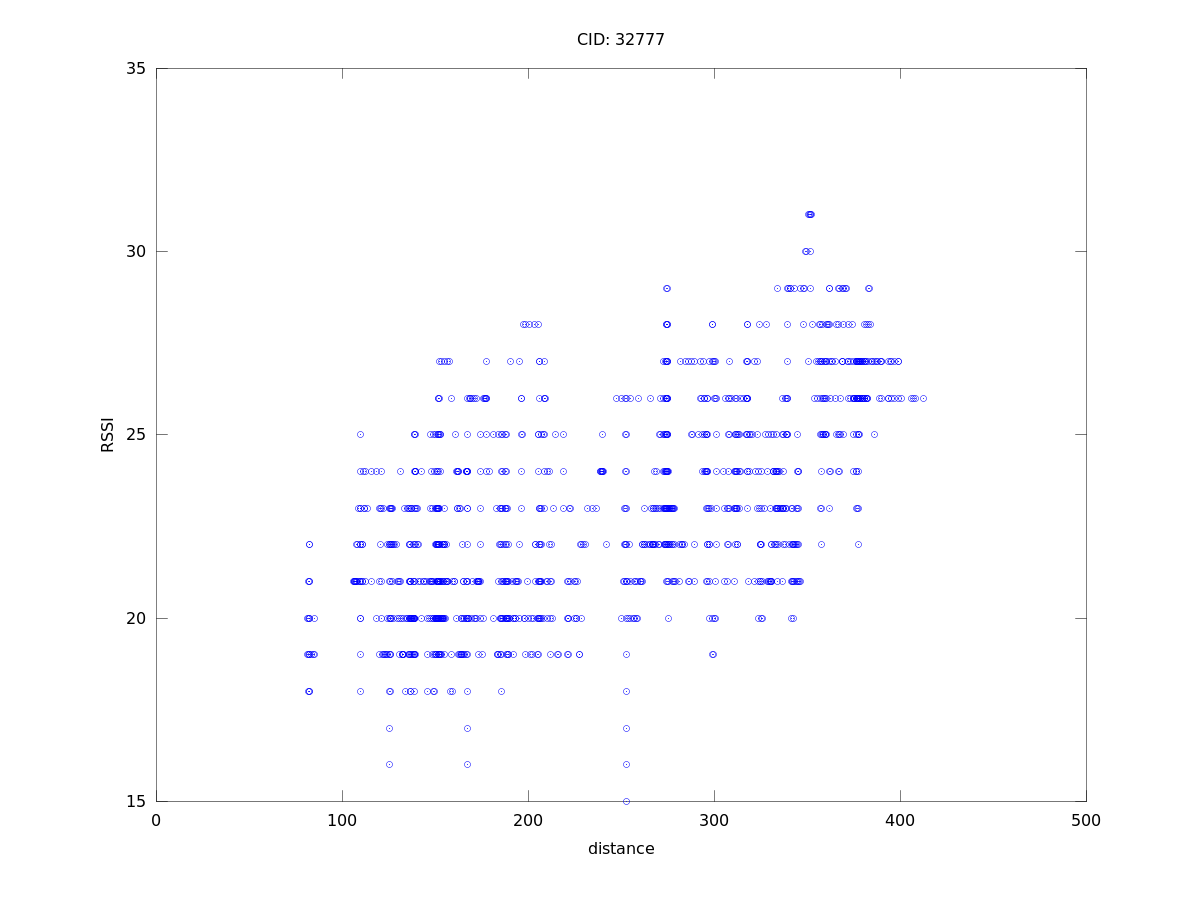
\includegraphics[width=1\textwidth]{cell32777raw.png}
		\end{subfigure}
		\begin{subfigure}[b]{0.3\textwidth}
			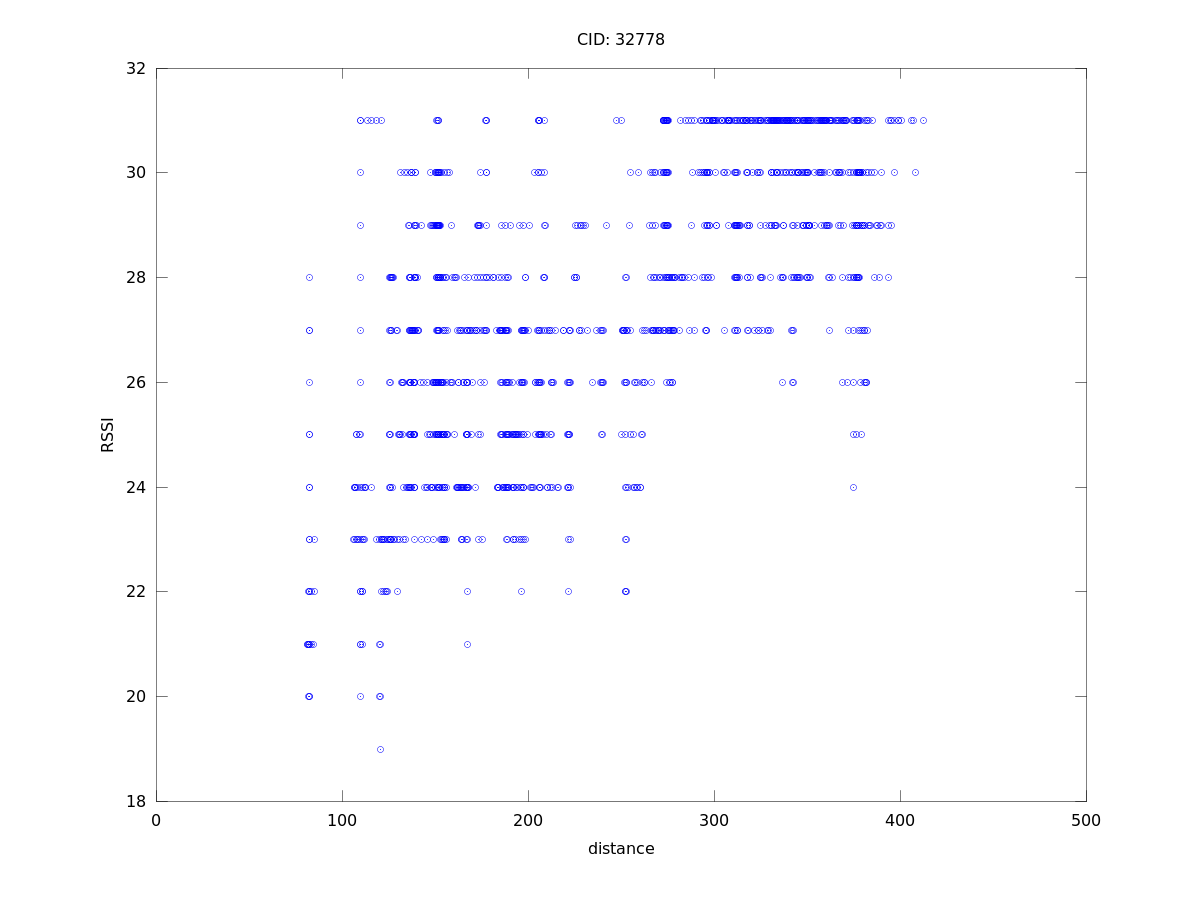
\includegraphics[width=1\textwidth]{cell32778raw.png}
		\end{subfigure}
		\begin{subfigure}[b]{0.3\textwidth}
			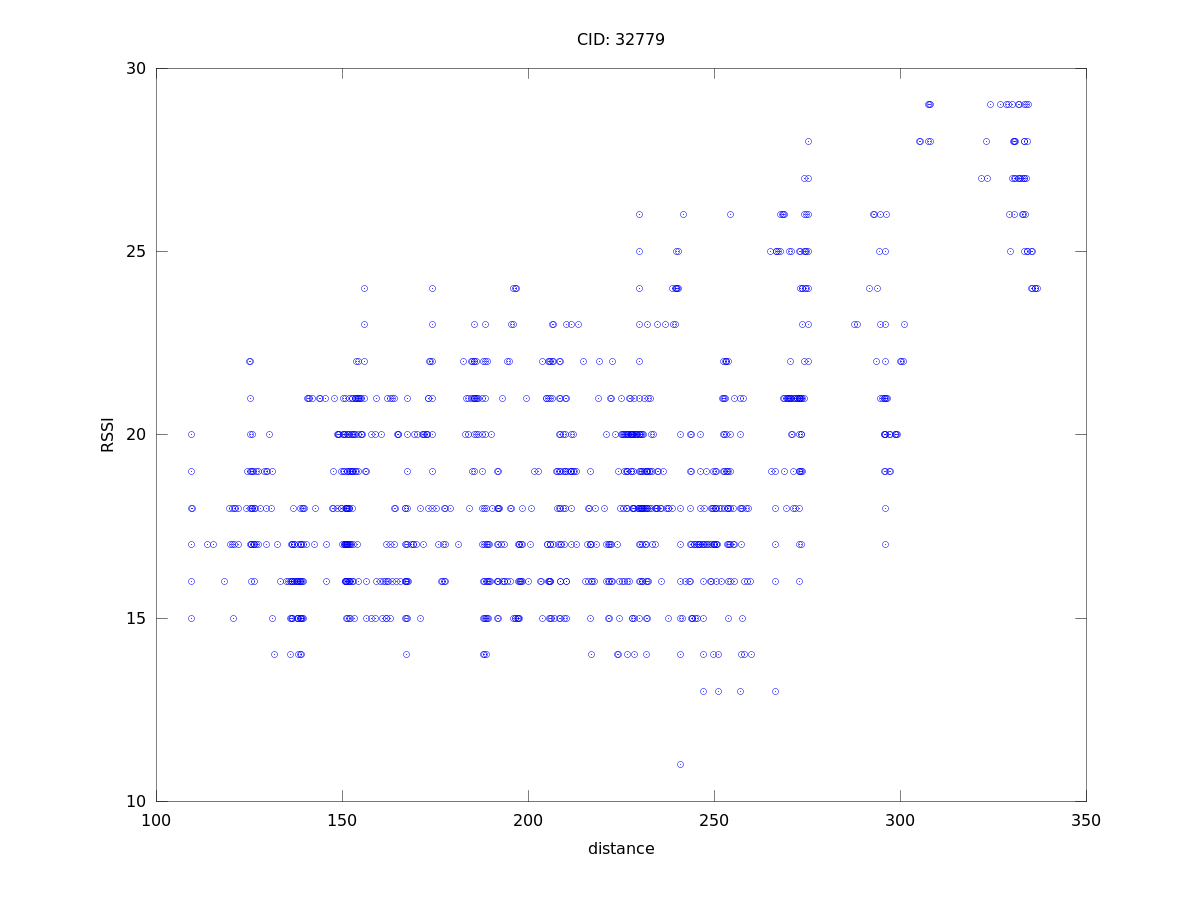
\includegraphics[width=1\textwidth]{cell32779raw.png}
		\end{subfigure}
	\end{center}
	\caption{Выборка данных для шести базовых станций, сигнал которых был принят позиционируемым устройством. Вертикальная ось --- asu, горизонтальная --- метры от начала маршрута.}
	\label{fig:exp-cell-raw}
\end{figure}

\subsection{Интерполяция}
\label{subsec:exp-interpol}
На данном этапе для выбранных множеств результатов предварительных замеров сигналов базовых станций строятся интерполяционные многочлены. На рис. \ref{fig:exp-cell-inter} приведены такие многочлены, степень каждого из которых определялась для каждой выборки индивидуально и равна одной десятой её длины. В пункте \ref{subsec:exp-order} вопрос выбора степени для интерполяционных многочленов рассмотрен более подробно.

\begin{figure}[p]
	\begin{center}
		\begin{subfigure}[b]{1\textwidth}
			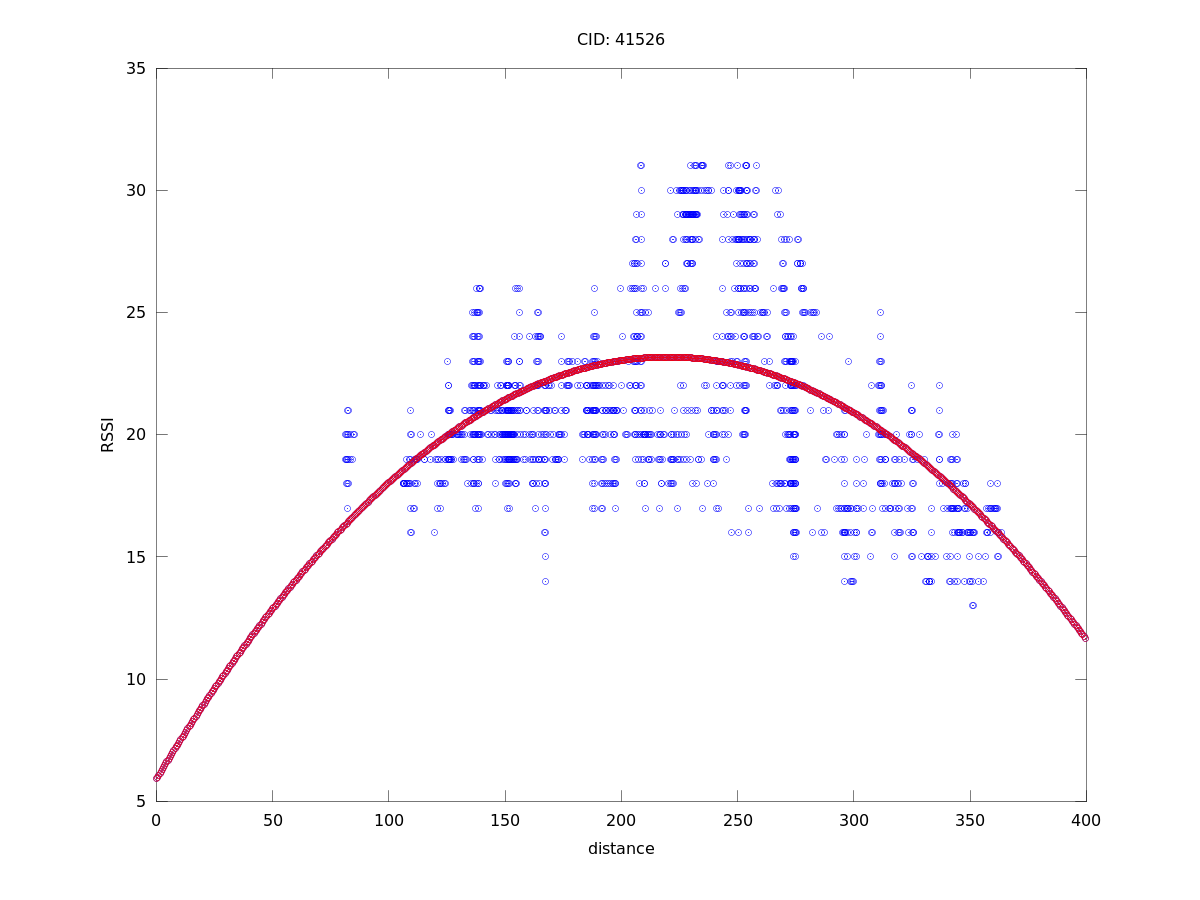
\includegraphics[width=1\textwidth]{cell41526inter.png}
		\end{subfigure}

		\begin{subfigure}[b]{0.45\textwidth}
			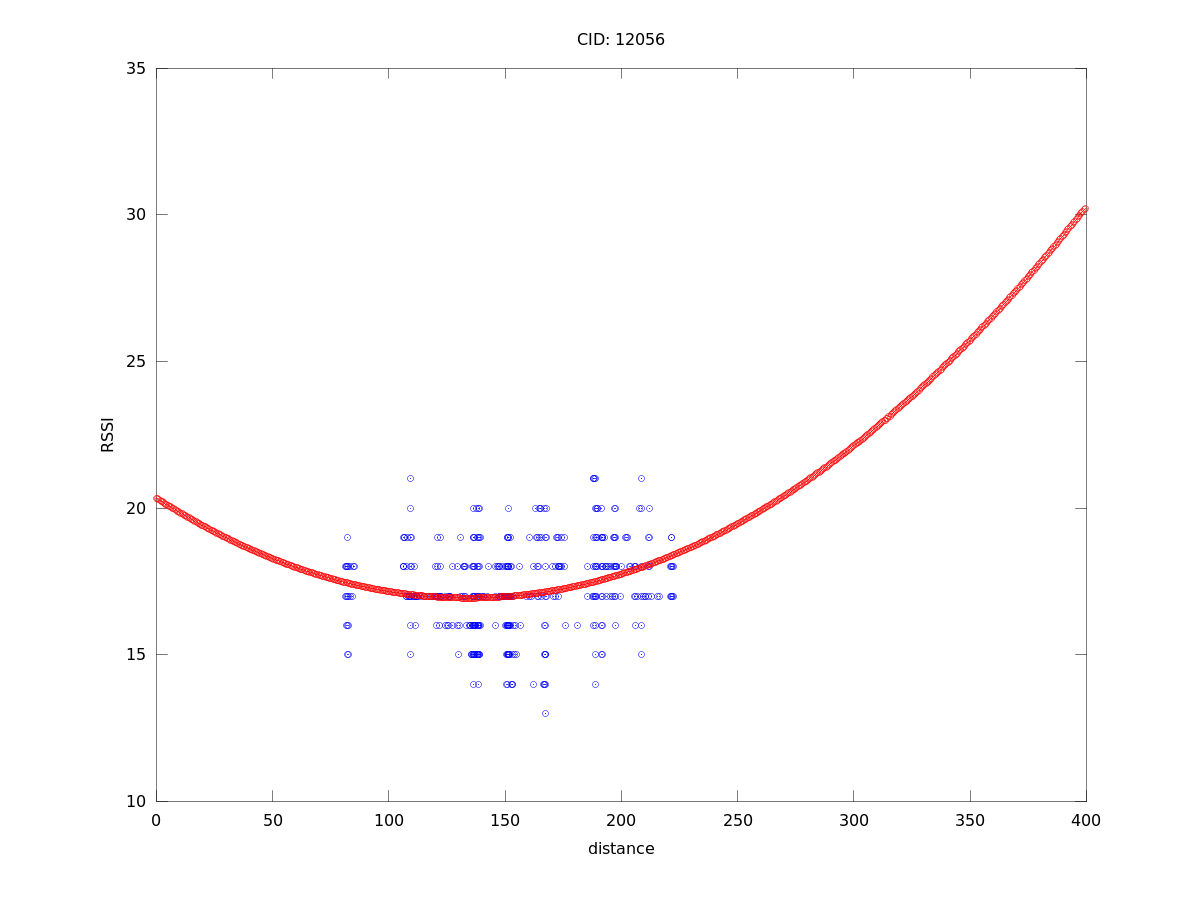
\includegraphics[width=1\textwidth]{cell12056inter.png}
		\end{subfigure}
		\begin{subfigure}[b]{0.45\textwidth}
			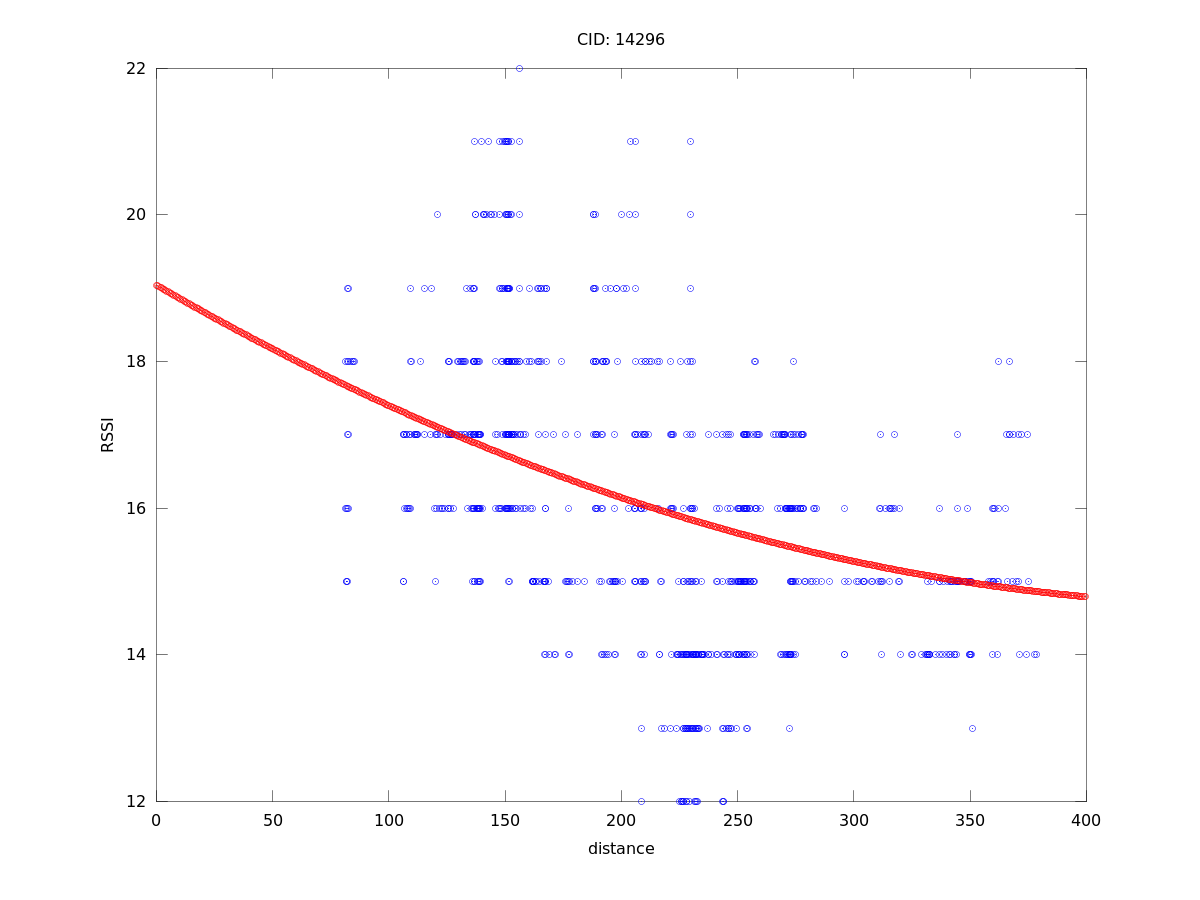
\includegraphics[width=1\textwidth]{cell14296inter.png}
		\end{subfigure}

		\begin{subfigure}[b]{0.3\textwidth}
			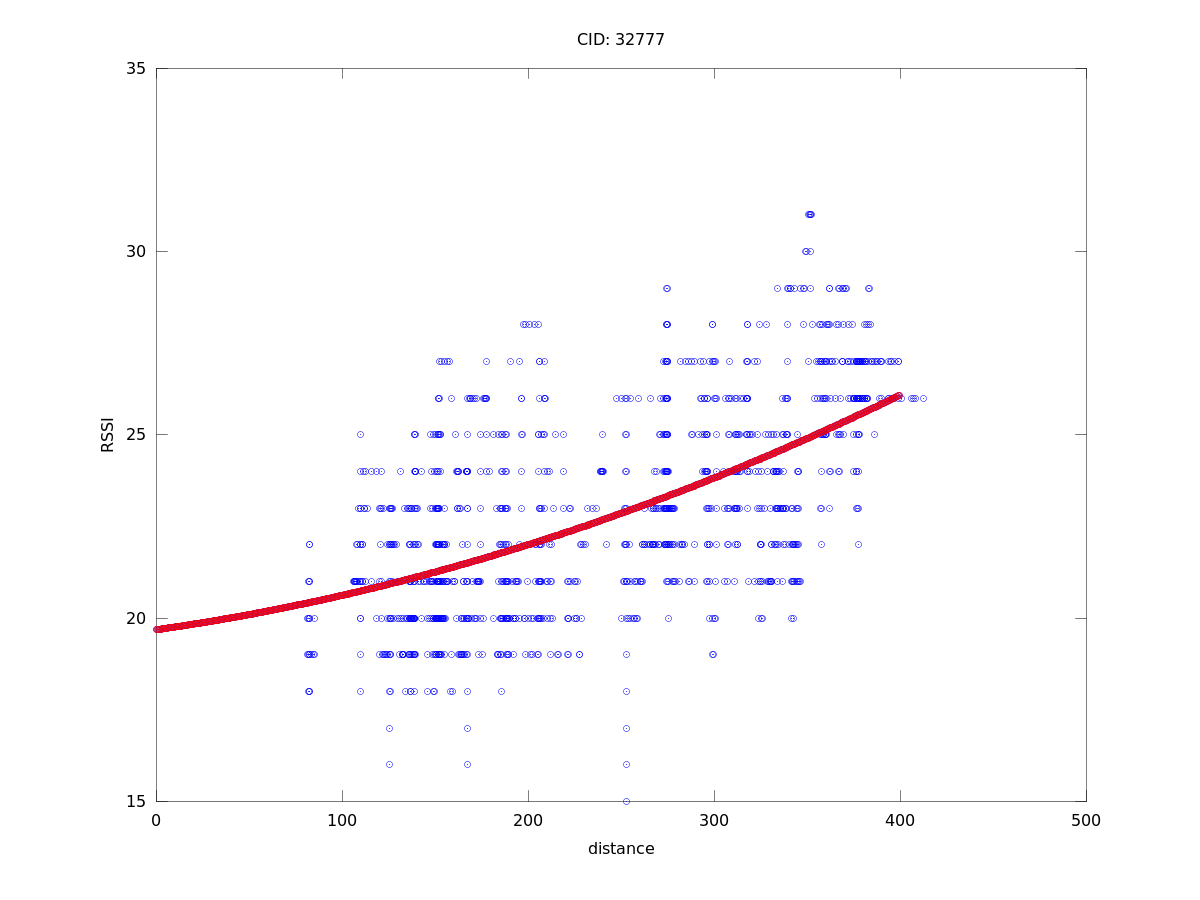
\includegraphics[width=1\textwidth]{cell32777inter.png}
		\end{subfigure}
		\begin{subfigure}[b]{0.3\textwidth}
			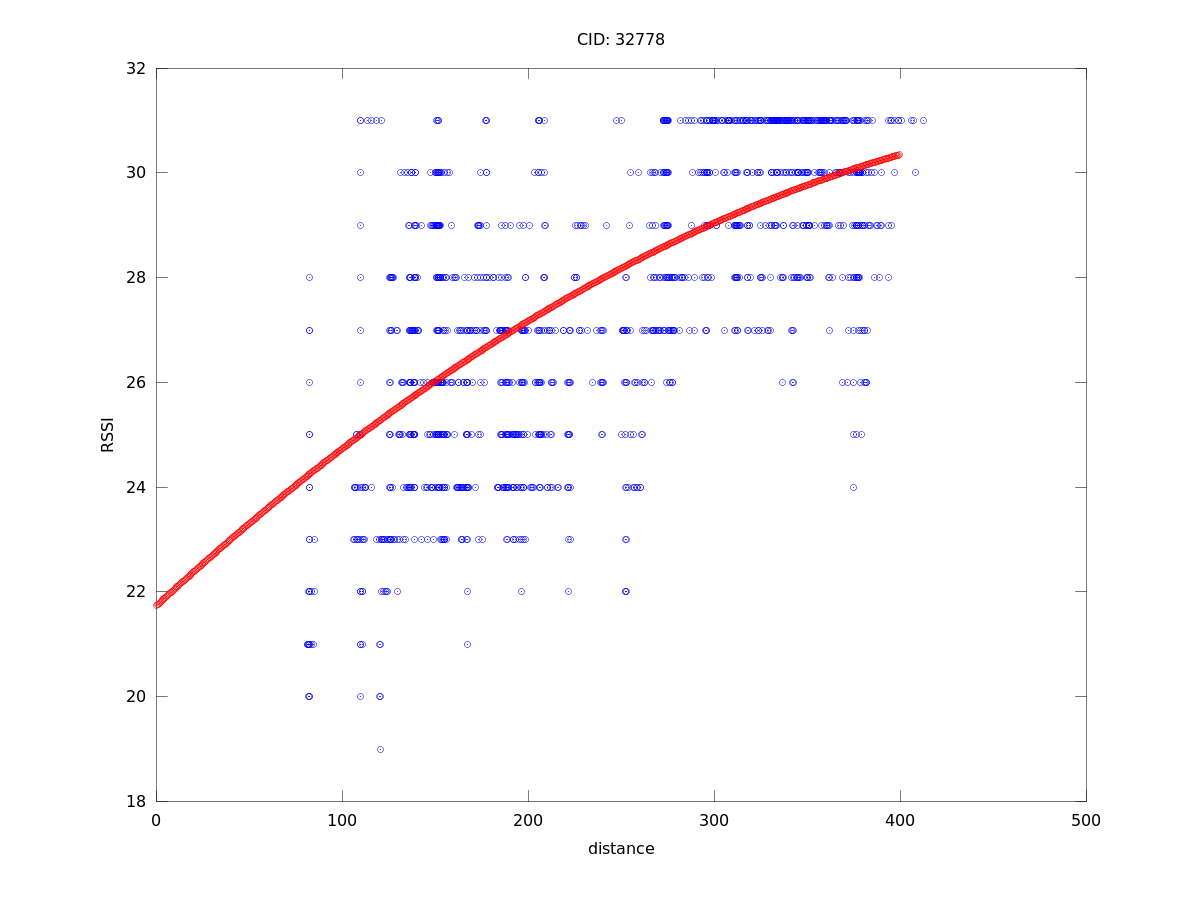
\includegraphics[width=1\textwidth]{cell32778inter.png}
		\end{subfigure}
		\begin{subfigure}[b]{0.3\textwidth}
			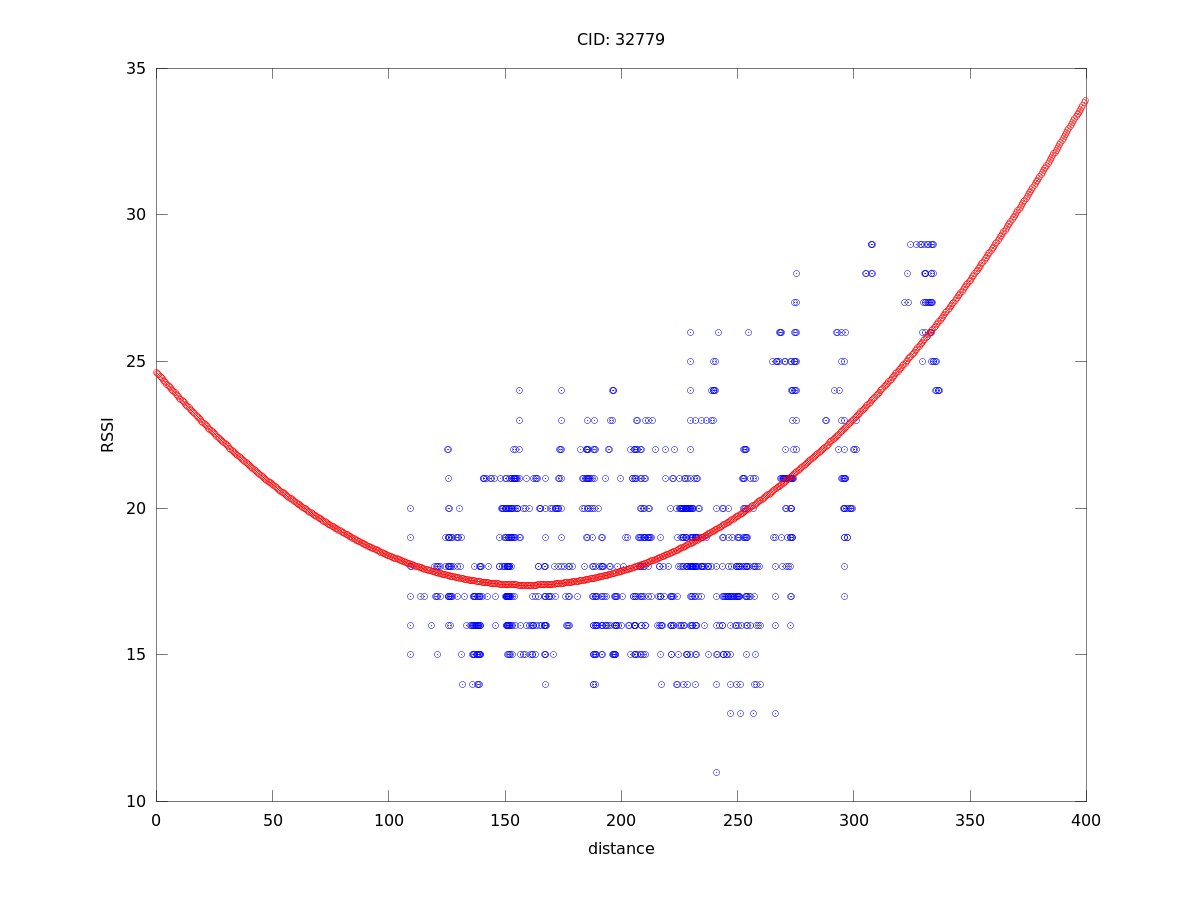
\includegraphics[width=1\textwidth]{cell32779inter.png}
		\end{subfigure}
	\end{center}
	\caption{Выборка данных о рассматриваемых станциях (точки) и интерполяционные многочлены для них (сплошные линии), полученные для степени, равной размерам выборок, делённым на 10. Вертикальная ось --- asu, горизонтальная --- метры от начала маршрута.}
	\label{fig:exp-cell-inter}
\end{figure}

\subsection{Псевдоплотности вероятности}

На данной стадии осуществляется сравнение статистических данных из базы, представленных в виде их интерполяционных многочленов, и фактически принятых RSSI. На рис. \ref{fig:exp-cell-pseudop} можно видеть, как приближение значения многочлена к фактически принятому ведёт к повышению значения псевдоплотности для данной точки.

\begin{figure}[p]
	\begin{center}
		\begin{subfigure}[b]{1\textwidth}
			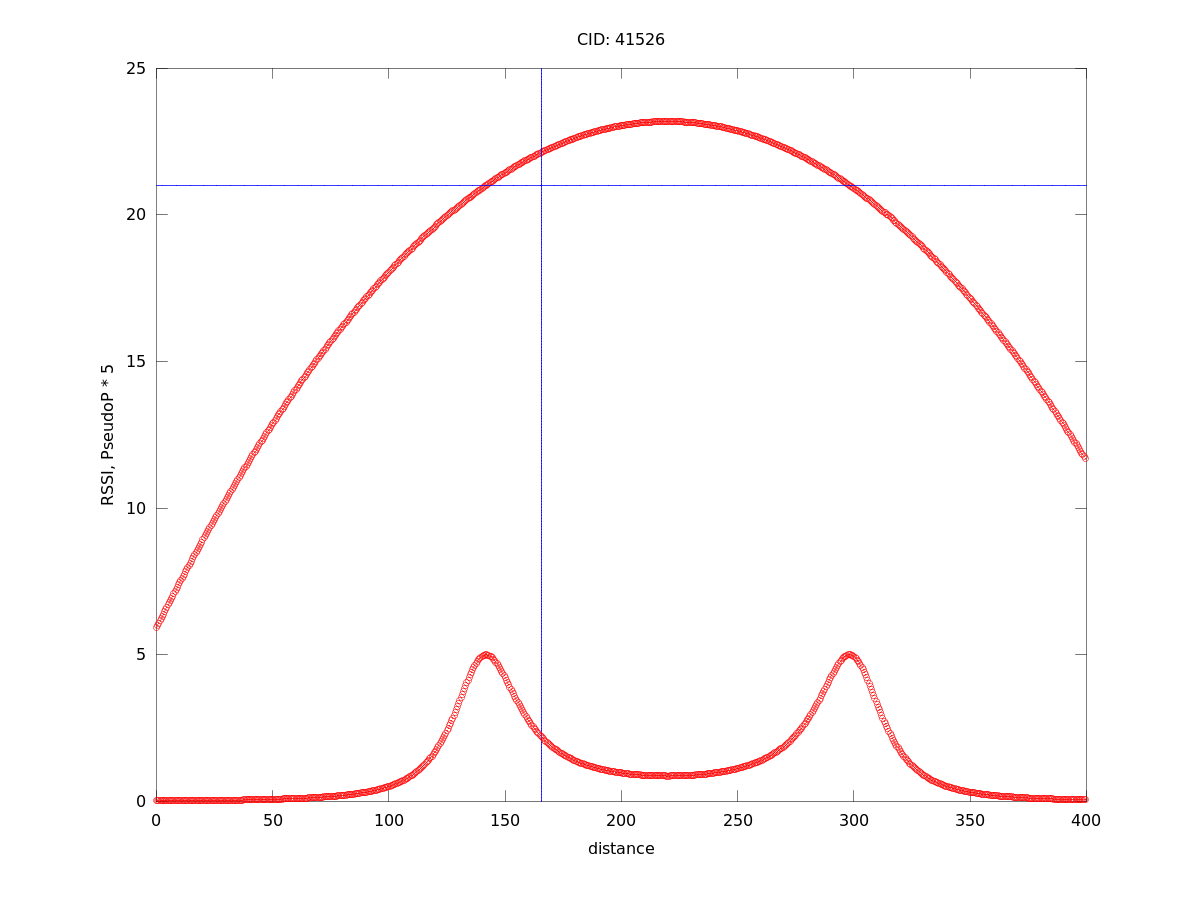
\includegraphics[width=1\textwidth]{cell41526pseudop.png}
		\end{subfigure}

		\begin{subfigure}[b]{0.4\textwidth}
			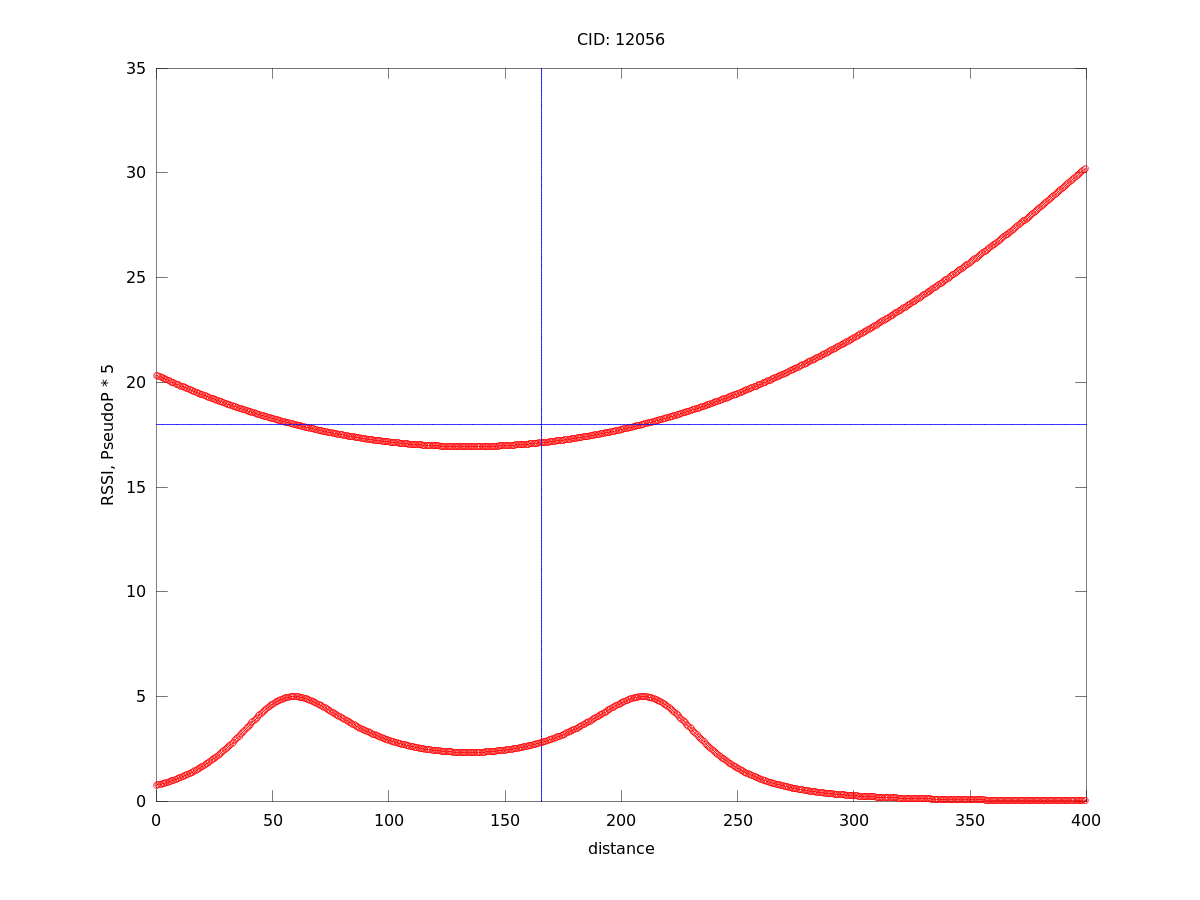
\includegraphics[width=1\textwidth]{cell12056pseudop.png}
		\end{subfigure}
		\begin{subfigure}[b]{0.4\textwidth}
			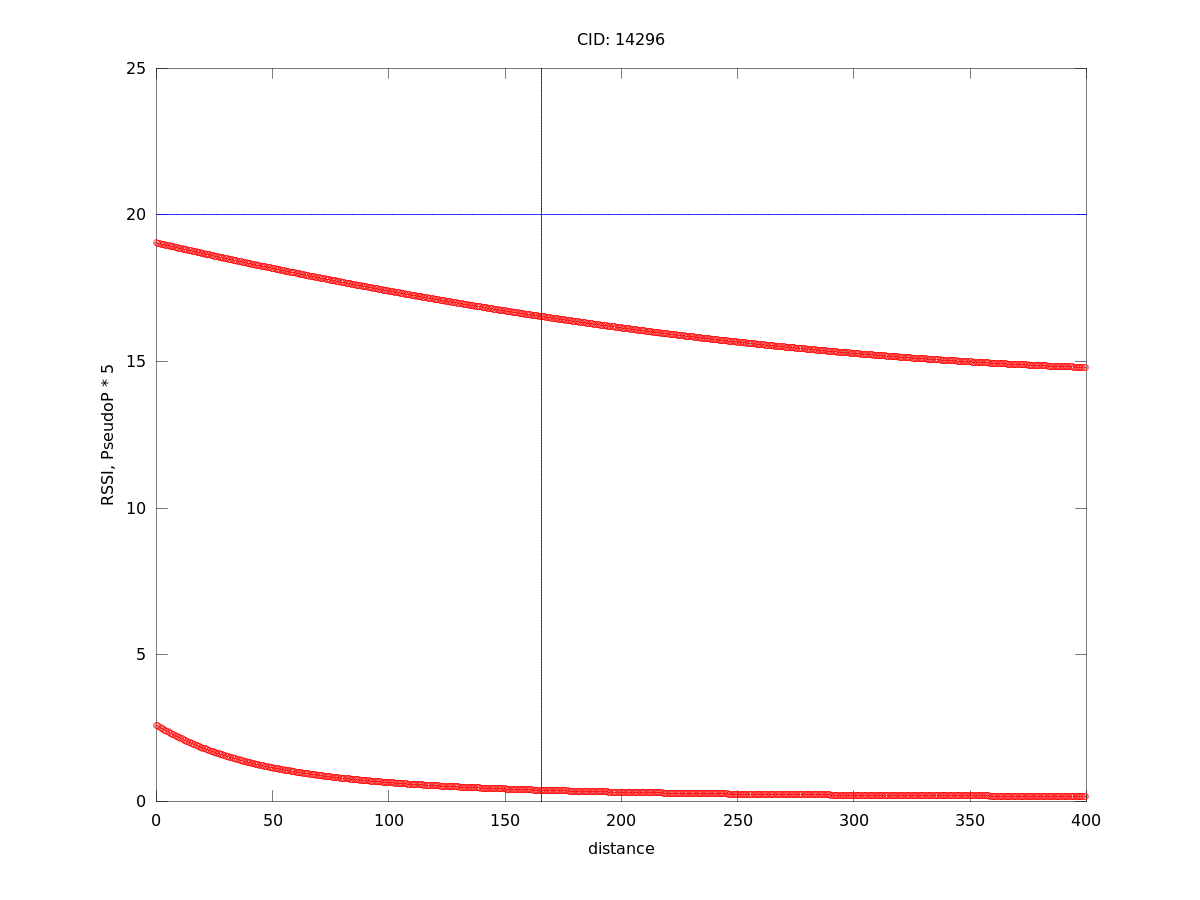
\includegraphics[width=1\textwidth]{cell14296pseudop.png}
		\end{subfigure}

		\begin{subfigure}[b]{0.25\textwidth}
			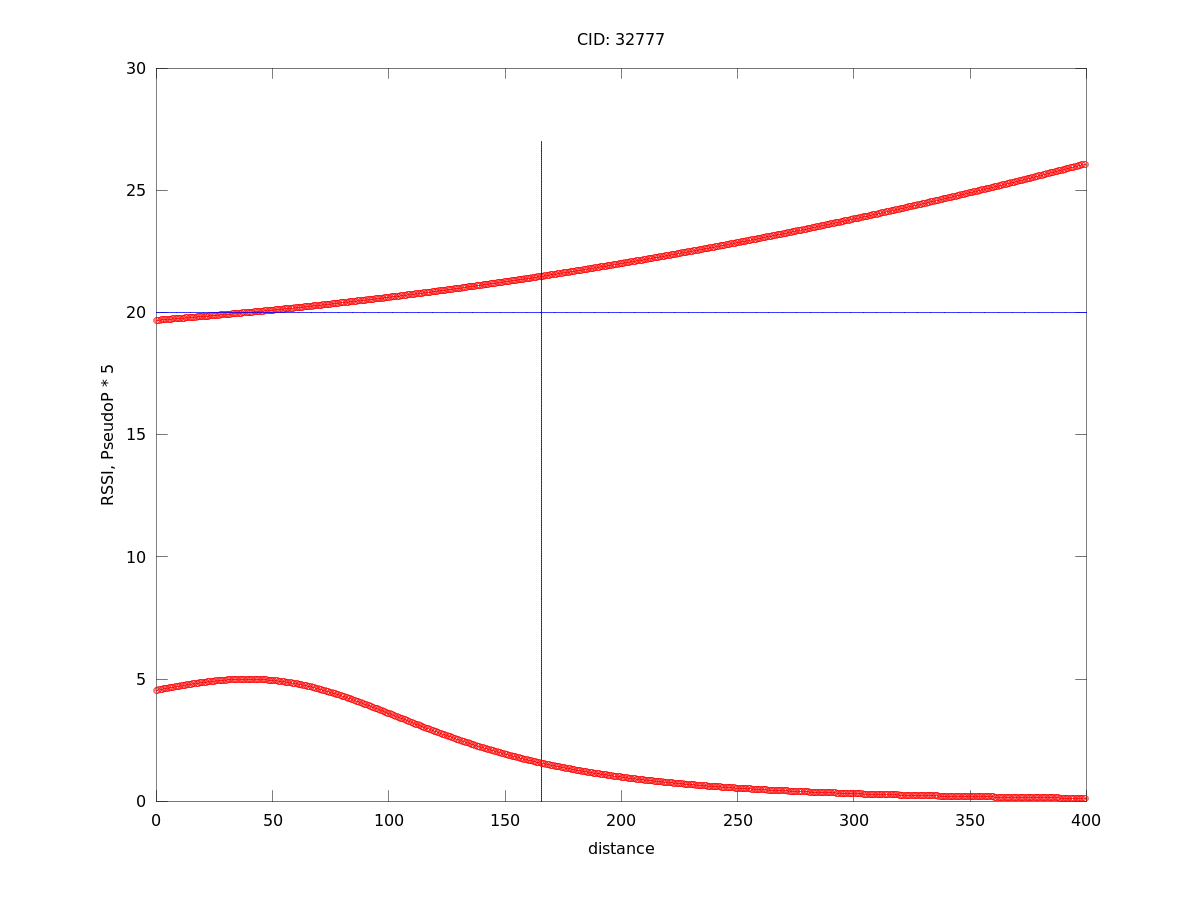
\includegraphics[width=1\textwidth]{cell32777pseudop.png}
		\end{subfigure}
		\begin{subfigure}[b]{0.25\textwidth}
			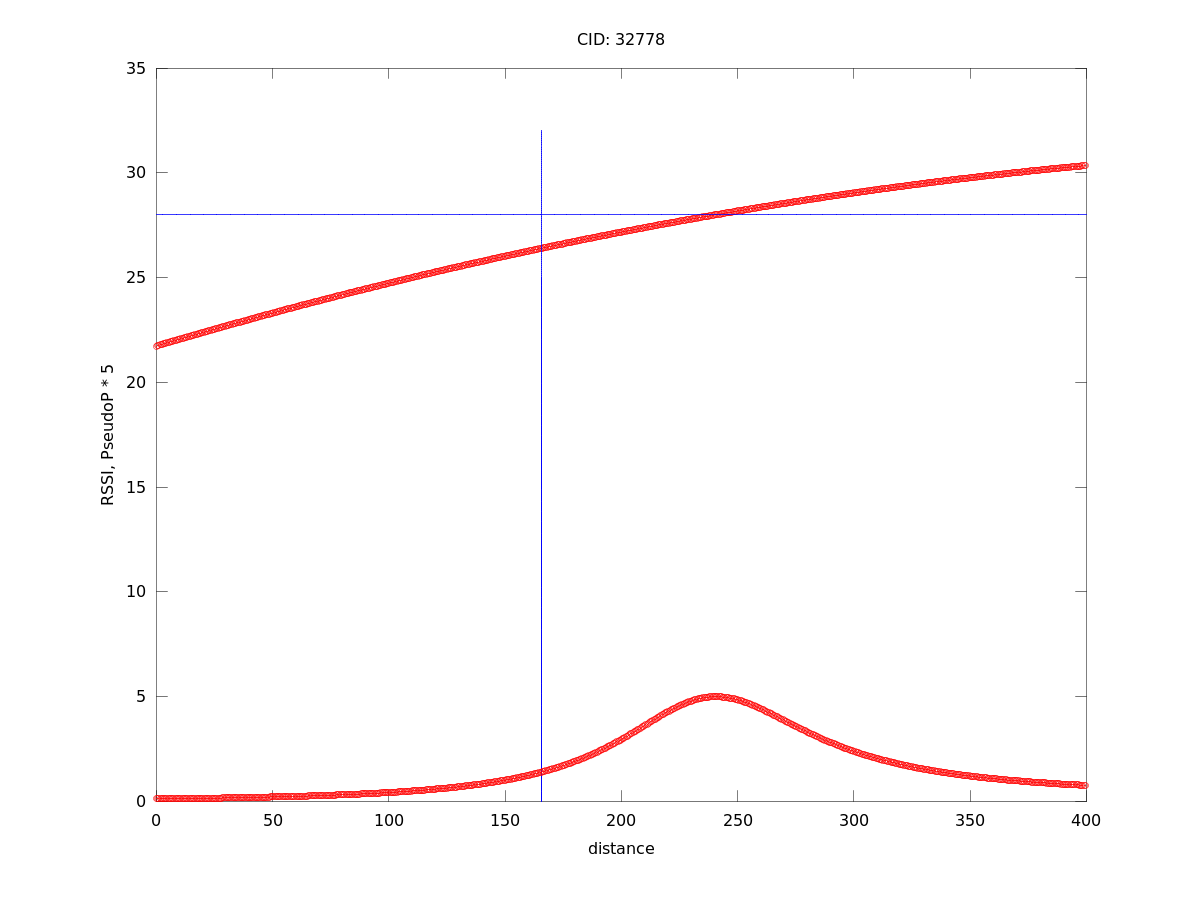
\includegraphics[width=1\textwidth]{cell32778pseudop.png}
		\end{subfigure}
		\begin{subfigure}[b]{0.25\textwidth}
			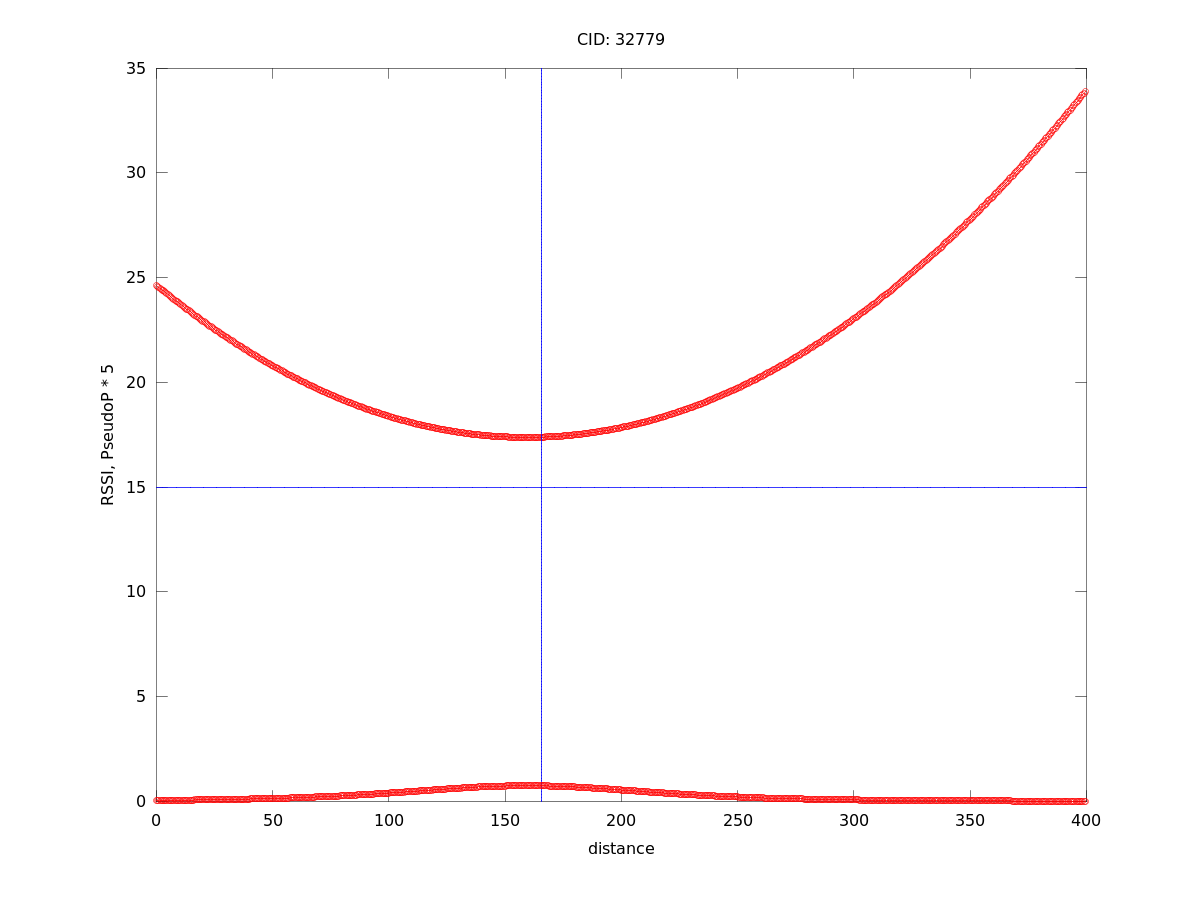
\includegraphics[width=1\textwidth]{cell32779pseudop.png}
		\end{subfigure}
	\end{center}
	\caption{Интерполяционные многочлены (толстая кривая сверху) и псевдоплотности вероятности (толстая кривая снизу) для принятых сигналов. Тонкая вертикальная прямая --- координата истинного положения, тонкая горизонтальная --- реально принятый RSSI для данной базовой станции. Вертикальная ось --- asu и единицы псевдоплотности, умноженные на 5, горизонтальная --- метры от начала маршрута.}
	\label{fig:exp-cell-pseudop}
\end{figure}

\subsection{Результирующая псевдоплотность}
\begin{figure}[h]
	\center{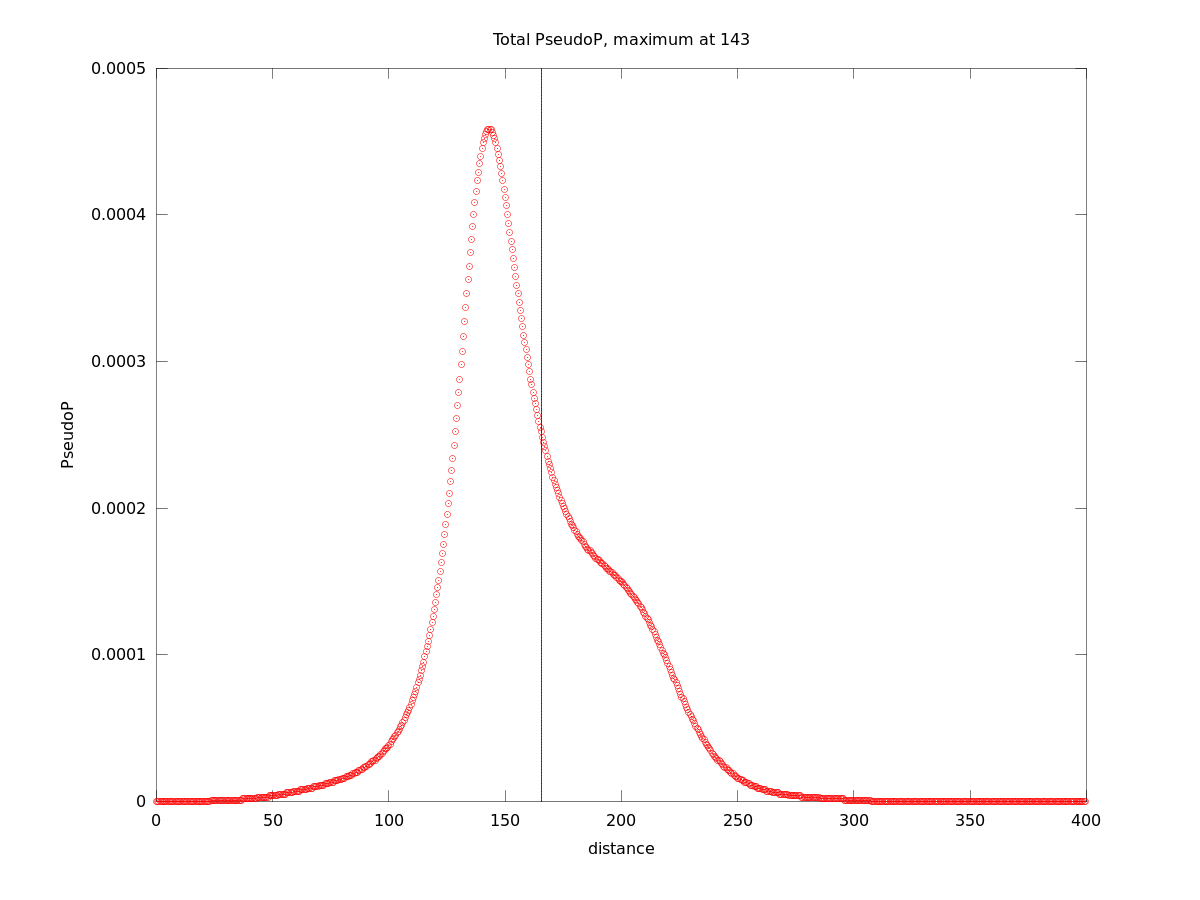
\includegraphics[width=1\linewidth]{totalpseudop.png}}
	\caption{Значения псевдоплотности в дискретно расположенных точках, обрабатывавшихся при поиске максимума. Вертикальная линия --- координата истинного положения устройства. Вертикальная ось --- единицы псевдоплотности, горизонтальная --- метры. Аргумент максимального положения --- 143 метра.}
	\label{fig:totalpseudop}
\end{figure}

Последний оставшийся шаг --- это перемножение независимо посчитанных псевдоплотностей для разных базовых станций между собой и поиск аргумента максимума полученной функции. На рис. \ref{fig:totalpseudop} изображена эта функция. Аргумента её максимума --- 143 метра, реальное положение устройства по данным GPS --- 165,5 метров. Итоговая ошибка составила 22,5 метров.

\section{Погрешность}
Перейдя от рассмотрения однократного процесса поиска местонахождения устройства к статистике этого процесса, рассмотрим, какое значение ошибки является типичным для реализованного алгоритма в условиях поставленного эксперимента.

\begin{figure}[h]
	\center{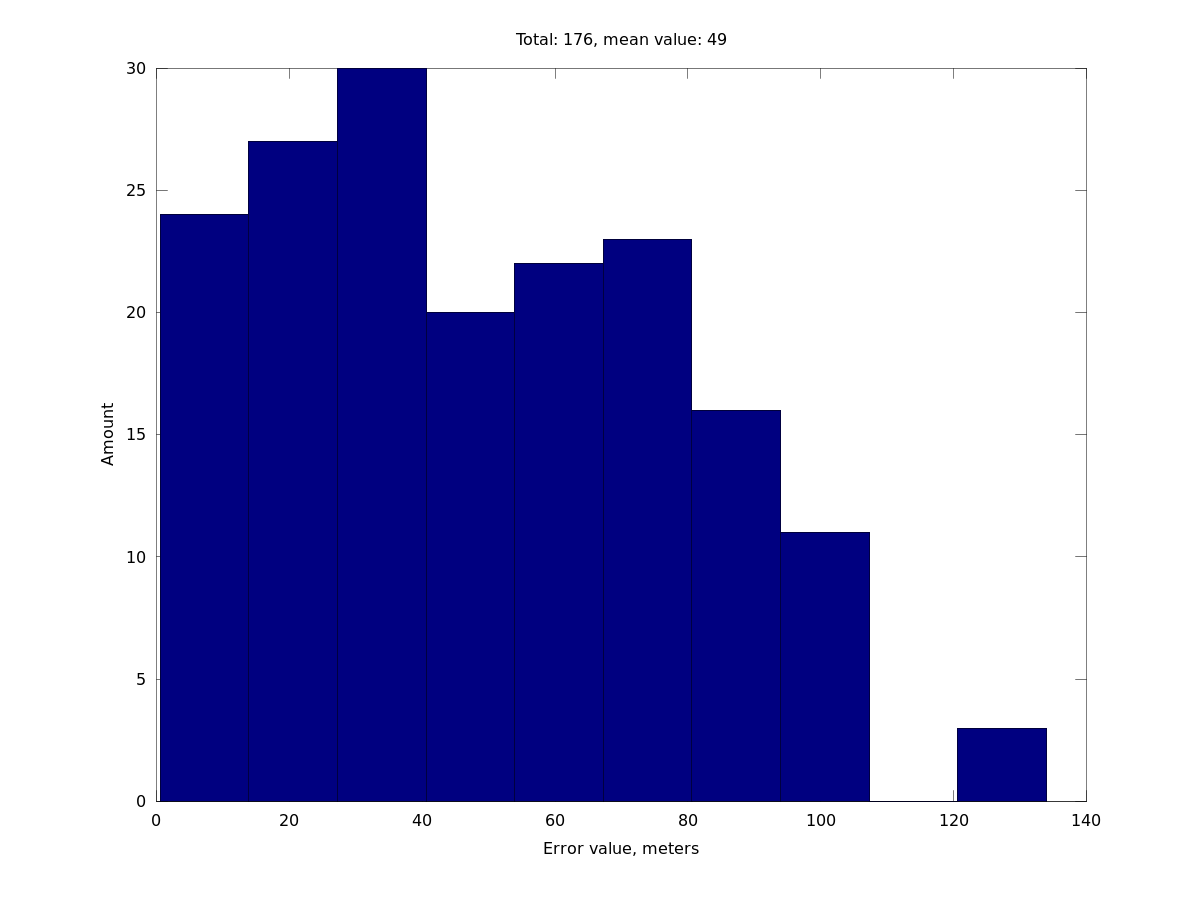
\includegraphics[width=1\linewidth]{errhist.png}}
	\caption{Гистограмма величин ошибок позиционирования. Горизонтальная ось --- величина ошибки в метрах, вертикальная --- количество появлений такой ошибки в экспериментах. Всего 176 примеров, математическое ожидание ошибки --- 49 метров.}
	\label{fig:errhist}
\end{figure}

Было поставлено 176 экспериментов, по возможности распределённых равномерно по всей длине маршрута. Для каждого из них отмечалось истинное значение расстояния от начала маршрута и результат его вычисления на основе данных GSM. После этого было вычислено расстояние между истинным и рассчитанным положением. Гистограмма полученной выборки изображена на рис. \ref{fig:errhist}. Математическое ожидание ошибки составило 49 метров.

\section{Анализ экспериментальных данных}

Точность позиционирования, достигнутая в ходе экспериментов, превышает современные системы, основанные на триангуляционном методе, но ещё не достигает точности спутниковых систем, что было бы идеальным результатом. Рассмотрим, какие факторы могут стоять на пути к повышению точности.

\subsection{Степени интерполяционных многочленов}
\label{subsec:exp-order}
Самый заметный из факторов видно на рис. \ref{fig:exp-cell-pseudop} --- очень простой вид полученных интерполяционных многочленов. Все они либо имеют лишь один видимый экстремум, либо позволяют предположить его наличие за пределами графиков (поскольку конечный многочлен с положительными степенями асимптотически сходиться к какому-либо конечному числу на может). Изначальная гипотеза предполагала наличие более сложного вида этой зависимости, который бы привёл к более выраженным экстремумам функции псевдоплотности вероятности и позволил достигнуть большей точности.

Проанализируем, с чем это может быть связано. В ходе процесса построения многочленов, описанного в пункте \ref{subsec:exp-interpol}, в качестве максимальной степени для каждого многочлена выбиралось значение, разное одной десятой размера выборки. Для разных базовых станций размеры выборок различаются, начинаясь от десятков замеров и заканчиваясь тысячами. Таким образом, и степени многочленов получаются существенным образом разные.

\begin{figure}[h]
	\begin{center}
		\begin{subfigure}[b]{0.45\textwidth}
			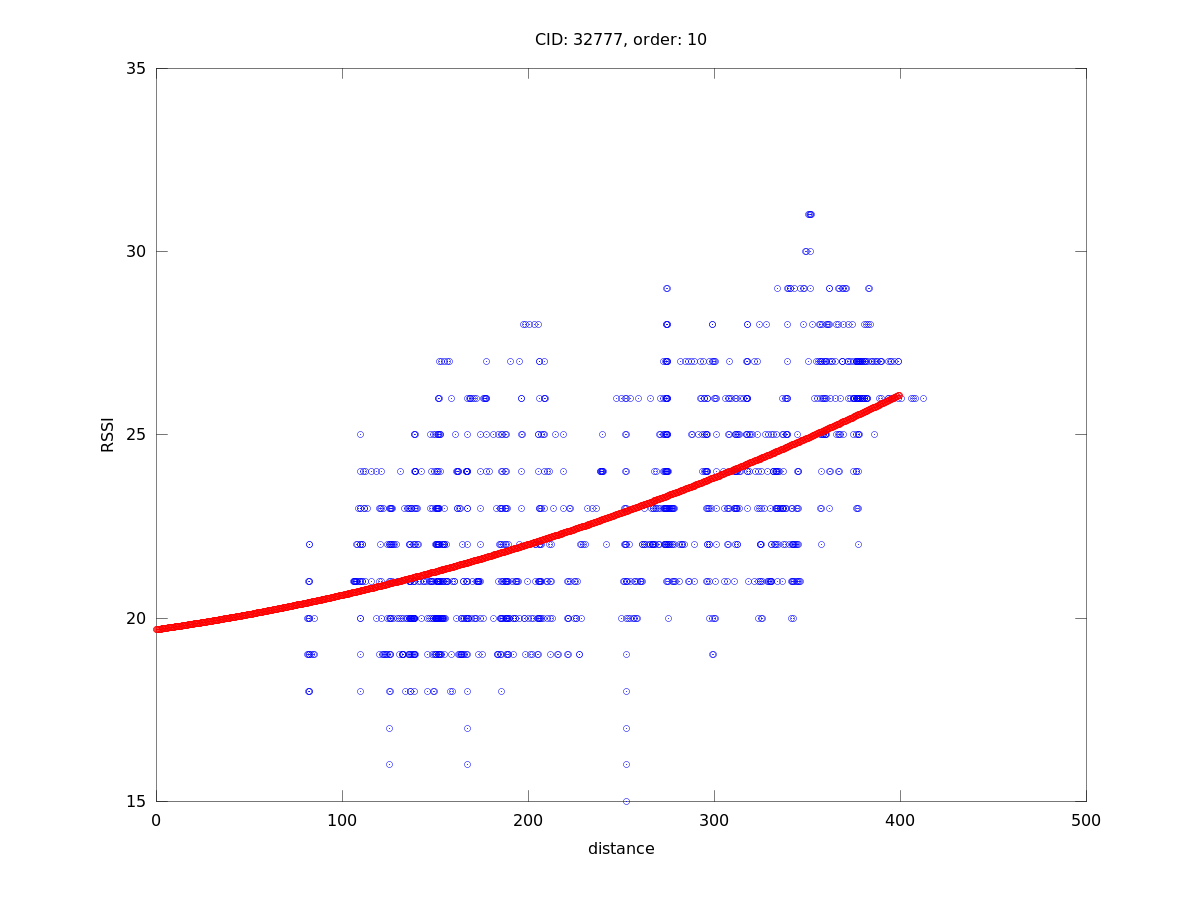
\includegraphics[width=1\textwidth]{cell32777inter10.png}
			\caption{Максимальная степень --- 10.}
		\end{subfigure}
		\begin{subfigure}[b]{0.45\textwidth}
			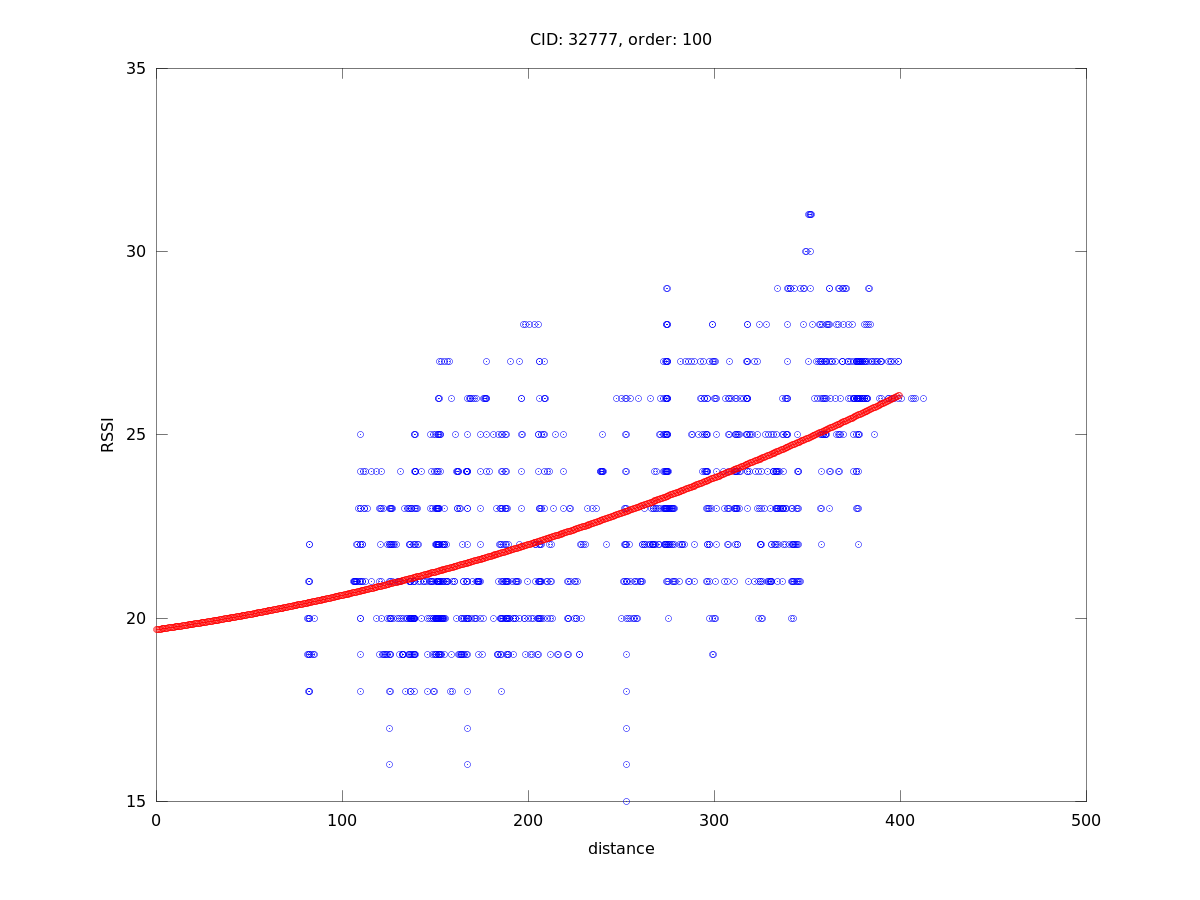
\includegraphics[width=1\textwidth]{cell32777inter100.png}
			\caption{Максимальная степень --- 100.}
		\end{subfigure}
	\end{center}
	\caption{Вид интерполяционных многочленов для выборки базовой станции 32777 при разной степени. Вертикальная ось --- asu, горизонтальная --- метры от начала маршрута.}
	\label{fig:exp-cell-order}
\end{figure}
Возьмём одну конкретную базовую станцию, пусть это будет 32777, для которой в базе имеется 2953 замеров, и построим для неё интерполяционные многочлены с разными степенями. На рис. \ref{fig:exp-cell-order} показаны интерполяционные многочлены десятой и сотой степени --- разницы между ними нет. Таким образом получается, что полученные в пункте \ref{subsec:exp-interpol} многочлены действительно являются лучшими полиномиальными приближениями имеющихся массивов данных (причём стоит отметить, что на отрезке 400 метров многочлен сотой степени может с большой точностью приблизить практически любую зависимость, имеющую физический смысл).

\subsection{Возможные дальнейшие эксперименты}
Итак, зависимость уровня от сигнала от расстояния до станции, выявленная в ходе экспериментов, имеет вид, отличающийся от теоретического предсказания, но имеет простой вид, а не обладает множеством экстремумов, порождённых отражениями сигнала, поглощением городской застройкой и прочими систематическими факторами. В связи с этим, важным вопросом, который должен быть выяснен в ходе дальнейших экспериментов, является такой: действительно ли погрешности носят преимущественно случайный характер, и в ходе экспериментов была выявлена единственная систематически наблюдаемая закономерность?

Одним из таких экспериментов видится следующий: сравнение статистических данных об уровнях сигнала в ряде точек с учётом и без учёта соседних. При многократных изменениях на первый план должны выйти именно постоянные факторы, а не случайные. Таким образом, если во многих точках, распределённых по маршруту, средние результаты многократных измерений будут сходиться к интерполяционному многочлену, даже несмотря на то, что измерения усредняются только по одной точке, в многочлен учитывает все, это будет сильным аргументом в пользу того, что выявленные зависимости являются единственными. И, следовательно, полученная точность близка к теоретическому пределу точности позиционирования, которую можно получить в сотовых сетях.

Если же такой сходимости наблюдаться не будет, это будет означать, что статистические методы как таковые могут работать точнее, но необходимо работать над совершенствованием методов, чтобы выявить дополнительные скрытые закономерности.

%This file is part of diplom-kovalev
%Copyright (C) 2012 Maxim Kovalev.
%Permission is granted to copy, distribute and/or modify this document
%under the terms of the GNU Free Documentation License, Version 1.3
%or any later version published by the Free Software Foundation;
%with no Invariant Sections, no Front-Cover Texts, and no Back-Cover Texts.
%A copy of the license is included in the section entitled "GNU
%Free Documentation License".

\chapter*{Заключение}
\addcontentsline{toc}{chapter}{Заключение}

В данной работе был предложен и опробован принципиально новый метод позиционирования устройств на основе сигналов базовых станций сетей GSM, рассчитанный на использование в системах наблюдения за наземным общественным транспортом. Качество работы метода превысило то, которое дают существующие, основанные на триангуляции в сетях GSM, но ещё не достигло точности, сравнимой со спутниковыми системами, а потому требуются и были предложены дополнительные экспериментальные и теоретические изыскания, направленные на дальнейшее совершенствование метода.

В обзорно-аналитической части были рассмотрены существующие методы позиционирования устройств: спутниковая навигация и триангуляция в сетях GSM. Были подробно исследованы особенности метода триангуляции и его практического применения, был сделан вывод о роли городской застройки как, предположительно, главного фактора, ограничивающего точность подобного метода. Было отмечено, что особенности общественного транспорта, как движущегося всегда по ограниченному и заранее известному набору маршрутов, позволяют отказаться от метода триангуляции, с присущими ему недостатками, в пользу статистических методов. Сформулирована гипотеза о том, что такой переход позволит значительно повысить точность позиционирования, возможно, вплоть до значений, обеспечиваемых спутниковой навигацией.

После этого был осуществлён анализ существующих методов поиска наибольшего правдоподобия аргумента при сравнении векторов случайных переменных, таких как расстояние Махаланобиса и Байесовский классификатор, в результате которого сделан вывод о том, что ни один из них в полной мере не удовлетворяет требованиям, предъявляемым к алгоритму позиционирования транспорта, хотя каждый из них обладает своими достоинствами, в результате чего сделан вывод о необходимости создания нового математического метода.

Создание требуемого алгоритма является одним из ключевых достижений данной работы. Была предложена функция псевдоплотности вероятности, позволяющая создать алгоритм, напоминающий Байесовский классификатор и обладающий всеми его достоинствами, такими как большая устойчивость к выбросам и шумам в значениях анализируемых случайных величин, но работающий с бесконечными, причём континуальными и упорядоченными множествами как возможных значений случайных величин, так и классов. Из возможности работы над континуальными множествами следует то, что алгоритм, во-первых, для каждой возможной точки учитывает не только данные о ней самой, но и данные о соседних точках, во-вторых, пользуется не дискретным сравнением совпадения данного ответа с хранящимся в базе, а использует нечёткую шкалу похожести, а в-третьих, позволяет успешно обрабатывать ситуацию, когда даётся ответ, никогда ранее не дававшийся, но похожий на имеющиеся.

Этот алгоритм был положен в основу прототипа программно-аппаратного комплекса для позиционирования, состоящего из четырёх звеньев:

\begin{enumerate}
	\item
		Мобильное устройство, собирающее данные об уровнях сигналов видимых базовых станций GSM в разных точках маршрута и передающее их на сервер; в качестве устройства использовался смартфон со специальной программой, написанной на языке Java и работающей под управлением ОС Android;
	\item
		Сервер, принимающий и сохраняющий данные об уровнях сигнала, а затем использующий их в работе созданного алгоритма позиционирования; написан на языке Python с использованием библиотеки NumPy для векторных вычислений;
	\item
		База данных, хранящая информацию об уровнях сигнала; использована СУБД MySQL;
	\item
		Клиентское приложение, получающее информацию о процессе сбора данных или позиционирования с сервера в реальном времени и отображающее её на карте местности; написано на языке Python с использованием библиотеки pygame для отображения графики.
\end{enumerate}

После завершения разработки системы была предложена методика проведения экспериментальной проверки гипотезы о возможности повышения точности позиционирования с использованием данной системы. Проверка осуществлялась на прямом тестовом участке на Покровском и Яузском бульварах в Москве. В ходе предварительного сбора данных было осуществлено боле 20 тысяч замеров уровней сигналов базовых станций в разных точках, при этом в разное время в зоне видимости были видны 22 различные базовые станции. Когда данные были собраны, было поставлено 176 экспериментов по позиционированию устройства, пользуясь собранными данными и разработанным алгоритмом, контроль при этом осуществлялся по данным GPS.

В результате, математическое ожидание ошибки позиционирования составило 49 метров, что лучше современных систем, основанных на триангуляционном методе, но ещё не достигает точности спутниковой навигации. На основании интерпретации экспериментальных данных, в том числе и трассировки процесса позиционирования на реальных данных, были выдвинуты гипотезы о факторах, которые могут мешать дальнейшему повышению точности, и предложены эксперименты для выяснения, возможно ли дальнейшее повышение точности с помощью статистических методов, или же был достигнут технологический предел точности позиционирования на основе данных об уровнях сигналов базовых станций.

{\bf{}Вывод} из данной работы можно сформулировать следующим образом: созданный математический метод показал большую точность позиционирования, чем триангуляция, и гипотеза о возможности повышения точности, используя статистический подход, оправдалась. При этом, достигнуть той точности, которую даёт спутниковая навигация, пока не удалось, но были предложены пути для дальнейшего совершенствования метода.

\newpage
\addcontentsline{toc}{chapter}{Литература}
\begin{flushleft}
	\bibliography{biblio}
\end{flushleft}

\label{chap:listoffigures}
\addcontentsline{toc}{chapter}{Список иллюстраций}
\listoffigures

\label{chap:listoftables}
\addcontentsline{toc}{chapter}{Список таблиц}
\listoftables

\chapter*{Список публикаций}
\label{chap:publications}
\addcontentsline{toc}{chapter}{Список публикаций}
\begin{enumerate}
	\item
		М.М.Ковалев. Позиционирование наземного транспорта с помощью сигнала GSM. Научно-техническая конференция студентов, аспирантов и молодых специалистов МИЭМ. Тезисы докладов. -- М.: МИЭМ, 2011. --- 420. ISBN 978-5-94506-257-3. с.с. 29--30.
	\item
		М.М.Ковалев. Прототип программно-аппаратного комплекса для сбора данных об уровнях сигнала GSM на местности. Научно-техническая конференция студентов, аспирантов и молодых специалистов МИЭМ, посвящённая 50-летию МИЭМ. Тезисы докладов. -- М.: МИЭМ, 2012. --- 445 с. ISBN 978-5-94506-314-3. с.с. 185--187.
\end{enumerate}

\begin{appendices}
	\titleformat{\chapter}[hang] 
	{\normalfont\huge\bfseries}{\chaptertitlename\ \thechapter.\ }{0em}{} 
	\renewcommand{\thechapter}{\arabic{chapter}}
%	\chapter{GNU Free Documentation License}
\label{label_fdl}

 \begin{center}

       Version 1.3, 3 November 2008


 Copyright \copyright{} 2000, 2001, 2002, 2007, 2008  Free Software Foundation, Inc.
 
 \bigskip
 
     \texttt{<http://fsf.org/>}
  
 \bigskip
 
 Everyone is permitted to copy and distribute verbatim copies
 of this license document, but changing it is not allowed.
\end{center}


\begin{center}
{\bf\large Preamble}
\end{center}

The purpose of this License is to make a manual, textbook, or other
functional and useful document ``free'' in the sense of freedom: to
assure everyone the effective freedom to copy and redistribute it,
with or without modifying it, either commercially or noncommercially.
Secondarily, this License preserves for the author and publisher a way
to get credit for their work, while not being considered responsible
for modifications made by others.

This License is a kind of ``copyleft'', which means that derivative
works of the document must themselves be free in the same sense.  It
complements the GNU General Public License, which is a copyleft
license designed for free software.

We have designed this License in order to use it for manuals for free
software, because free software needs free documentation: a free
program should come with manuals providing the same freedoms that the
software does.  But this License is not limited to software manuals;
it can be used for any textual work, regardless of subject matter or
whether it is published as a printed book.  We recommend this License
principally for works whose purpose is instruction or reference.


\begin{center}
{\Large\bf 1. APPLICABILITY AND DEFINITIONS\par}
\phantomsection
%\addcontentsline{toc}{section}{1. APPLICABILITY AND DEFINITIONS}
\end{center}

This License applies to any manual or other work, in any medium, that
contains a notice placed by the copyright holder saying it can be
distributed under the terms of this License.  Such a notice grants a
world-wide, royalty-free license, unlimited in duration, to use that
work under the conditions stated herein.  The ``\textbf{Document}'', below,
refers to any such manual or work.  Any member of the public is a
licensee, and is addressed as ``\textbf{you}''.  You accept the license if you
copy, modify or distribute the work in a way requiring permission
under copyright law.

A ``\textbf{Modified Version}'' of the Document means any work containing the
Document or a portion of it, either copied verbatim, or with
modifications and/or translated into another language.

A ``\textbf{Secondary Section}'' is a named appendix or a front-matter section of
the Document that deals exclusively with the relationship of the
publishers or authors of the Document to the Document's overall subject
(or to related matters) and contains nothing that could fall directly
within that overall subject.  (Thus, if the Document is in part a
textbook of mathematics, a Secondary Section may not explain any
mathematics.)  The relationship could be a matter of historical
connection with the subject or with related matters, or of legal,
commercial, philosophical, ethical or political position regarding
them.

The ``\textbf{Invariant Sections}'' are certain Secondary Sections whose titles
are designated, as being those of Invariant Sections, in the notice
that says that the Document is released under this License.  If a
section does not fit the above definition of Secondary then it is not
allowed to be designated as Invariant.  The Document may contain zero
Invariant Sections.  If the Document does not identify any Invariant
Sections then there are none.

The ``\textbf{Cover Texts}'' are certain short passages of text that are listed,
as Front-Cover Texts or Back-Cover Texts, in the notice that says that
the Document is released under this License.  A Front-Cover Text may
be at most 5 words, and a Back-Cover Text may be at most 25 words.

A ``\textbf{Transparent}'' copy of the Document means a machine-readable copy,
represented in a format whose specification is available to the
general public, that is suitable for revising the document
straightforwardly with generic text editors or (for images composed of
pixels) generic paint programs or (for drawings) some widely available
drawing editor, and that is suitable for input to text formatters or
for automatic translation to a variety of formats suitable for input
to text formatters.  A copy made in an otherwise Transparent file
format whose markup, or absence of markup, has been arranged to thwart
or discourage subsequent modification by readers is not Transparent.
An image format is not Transparent if used for any substantial amount
of text.  A copy that is not ``Transparent'' is called ``\textbf{Opaque}''.

Examples of suitable formats for Transparent copies include plain
ASCII without markup, Texinfo input format, LaTeX input format, SGML
or XML using a publicly available DTD, and standard-conforming simple
HTML, PostScript or PDF designed for human modification.  Examples of
transparent image formats include PNG, XCF and JPG.  Opaque formats
include proprietary formats that can be read and edited only by
proprietary word processors, SGML or XML for which the DTD and/or
processing tools are not generally available, and the
machine-generated HTML, PostScript or PDF produced by some word
processors for output purposes only.

The ``\textbf{Title Page}'' means, for a printed book, the title page itself,
plus such following pages as are needed to hold, legibly, the material
this License requires to appear in the title page.  For works in
formats which do not have any title page as such, ``Title Page'' means
the text near the most prominent appearance of the work's title,
preceding the beginning of the body of the text.

The ``\textbf{publisher}'' means any person or entity that distributes
copies of the Document to the public.

A section ``\textbf{Entitled XYZ}'' means a named subunit of the Document whose
title either is precisely XYZ or contains XYZ in parentheses following
text that translates XYZ in another language.  (Here XYZ stands for a
specific section name mentioned below, such as ``\textbf{Acknowledgements}'',
``\textbf{Dedications}'', ``\textbf{Endorsements}'', or ``\textbf{History}''.)  
To ``\textbf{Preserve the Title}''
of such a section when you modify the Document means that it remains a
section ``Entitled XYZ'' according to this definition.

The Document may include Warranty Disclaimers next to the notice which
states that this License applies to the Document.  These Warranty
Disclaimers are considered to be included by reference in this
License, but only as regards disclaiming warranties: any other
implication that these Warranty Disclaimers may have is void and has
no effect on the meaning of this License.


\begin{center}
{\Large\bf 2. VERBATIM COPYING\par}
\phantomsection
%\addcontentsline{toc}{section}{2. VERBATIM COPYING}
\end{center}

You may copy and distribute the Document in any medium, either
commercially or noncommercially, provided that this License, the
copyright notices, and the license notice saying this License applies
to the Document are reproduced in all copies, and that you add no other
conditions whatsoever to those of this License.  You may not use
technical measures to obstruct or control the reading or further
copying of the copies you make or distribute.  However, you may accept
compensation in exchange for copies.  If you distribute a large enough
number of copies you must also follow the conditions in section~3.

You may also lend copies, under the same conditions stated above, and
you may publicly display copies.


\begin{center}
{\Large\bf 3. COPYING IN QUANTITY\par}
\phantomsection
%\addcontentsline{toc}{section}{3. COPYING IN QUANTITY}
\end{center}


If you publish printed copies (or copies in media that commonly have
printed covers) of the Document, numbering more than 100, and the
Document's license notice requires Cover Texts, you must enclose the
copies in covers that carry, clearly and legibly, all these Cover
Texts: Front-Cover Texts on the front cover, and Back-Cover Texts on
the back cover.  Both covers must also clearly and legibly identify
you as the publisher of these copies.  The front cover must present
the full title with all words of the title equally prominent and
visible.  You may add other material on the covers in addition.
Copying with changes limited to the covers, as long as they preserve
the title of the Document and satisfy these conditions, can be treated
as verbatim copying in other respects.

If the required texts for either cover are too voluminous to fit
legibly, you should put the first ones listed (as many as fit
reasonably) on the actual cover, and continue the rest onto adjacent
pages.

If you publish or distribute Opaque copies of the Document numbering
more than 100, you must either include a machine-readable Transparent
copy along with each Opaque copy, or state in or with each Opaque copy
a computer-network location from which the general network-using
public has access to download using public-standard network protocols
a complete Transparent copy of the Document, free of added material.
If you use the latter option, you must take reasonably prudent steps,
when you begin distribution of Opaque copies in quantity, to ensure
that this Transparent copy will remain thus accessible at the stated
location until at least one year after the last time you distribute an
Opaque copy (directly or through your agents or retailers) of that
edition to the public.

It is requested, but not required, that you contact the authors of the
Document well before redistributing any large number of copies, to give
them a chance to provide you with an updated version of the Document.


\begin{center}
{\Large\bf 4. MODIFICATIONS\par}
\phantomsection
%\addcontentsline{toc}{section}{4. MODIFICATIONS}
\end{center}

You may copy and distribute a Modified Version of the Document under
the conditions of sections 2 and 3 above, provided that you release
the Modified Version under precisely this License, with the Modified
Version filling the role of the Document, thus licensing distribution
and modification of the Modified Version to whoever possesses a copy
of it.  In addition, you must do these things in the Modified Version:

\begin{itemize}
\item[A.] 
   Use in the Title Page (and on the covers, if any) a title distinct
   from that of the Document, and from those of previous versions
   (which should, if there were any, be listed in the History section
   of the Document).  You may use the same title as a previous version
   if the original publisher of that version gives permission.
   
\item[B.]
   List on the Title Page, as authors, one or more persons or entities
   responsible for authorship of the modifications in the Modified
   Version, together with at least five of the principal authors of the
   Document (all of its principal authors, if it has fewer than five),
   unless they release you from this requirement.
   
\item[C.]
   State on the Title page the name of the publisher of the
   Modified Version, as the publisher.
   
\item[D.]
   Preserve all the copyright notices of the Document.
   
\item[E.]
   Add an appropriate copyright notice for your modifications
   adjacent to the other copyright notices.
   
\item[F.]
   Include, immediately after the copyright notices, a license notice
   giving the public permission to use the Modified Version under the
   terms of this License, in the form shown in the Addendum below.
   
\item[G.]
   Preserve in that license notice the full lists of Invariant Sections
   and required Cover Texts given in the Document's license notice.
   
\item[H.]
   Include an unaltered copy of this License.
   
\item[I.]
   Preserve the section Entitled ``History'', Preserve its Title, and add
   to it an item stating at least the title, year, new authors, and
   publisher of the Modified Version as given on the Title Page.  If
   there is no section Entitled ``History'' in the Document, create one
   stating the title, year, authors, and publisher of the Document as
   given on its Title Page, then add an item describing the Modified
   Version as stated in the previous sentence.
   
\item[J.]
   Preserve the network location, if any, given in the Document for
   public access to a Transparent copy of the Document, and likewise
   the network locations given in the Document for previous versions
   it was based on.  These may be placed in the ``History'' section.
   You may omit a network location for a work that was published at
   least four years before the Document itself, or if the original
   publisher of the version it refers to gives permission.
   
\item[K.]
   For any section Entitled ``Acknowledgements'' or ``Dedications'',
   Preserve the Title of the section, and preserve in the section all
   the substance and tone of each of the contributor acknowledgements
   and/or dedications given therein.
   
\item[L.]
   Preserve all the Invariant Sections of the Document,
   unaltered in their text and in their titles.  Section numbers
   or the equivalent are not considered part of the section titles.
   
\item[M.]
   Delete any section Entitled ``Endorsements''.  Such a section
   may not be included in the Modified Version.
   
\item[N.]
   Do not retitle any existing section to be Entitled ``Endorsements''
   or to conflict in title with any Invariant Section.
   
\item[O.]
   Preserve any Warranty Disclaimers.
\end{itemize}

If the Modified Version includes new front-matter sections or
appendices that qualify as Secondary Sections and contain no material
copied from the Document, you may at your option designate some or all
of these sections as invariant.  To do this, add their titles to the
list of Invariant Sections in the Modified Version's license notice.
These titles must be distinct from any other section titles.

You may add a section Entitled ``Endorsements'', provided it contains
nothing but endorsements of your Modified Version by various
parties---for example, statements of peer review or that the text has
been approved by an organization as the authoritative definition of a
standard.

You may add a passage of up to five words as a Front-Cover Text, and a
passage of up to 25 words as a Back-Cover Text, to the end of the list
of Cover Texts in the Modified Version.  Only one passage of
Front-Cover Text and one of Back-Cover Text may be added by (or
through arrangements made by) any one entity.  If the Document already
includes a cover text for the same cover, previously added by you or
by arrangement made by the same entity you are acting on behalf of,
you may not add another; but you may replace the old one, on explicit
permission from the previous publisher that added the old one.

The author(s) and publisher(s) of the Document do not by this License
give permission to use their names for publicity for or to assert or
imply endorsement of any Modified Version.


\begin{center}
{\Large\bf 5. COMBINING DOCUMENTS\par}
\phantomsection
%\addcontentsline{toc}{section}{5. COMBINING DOCUMENTS}
\end{center}


You may combine the Document with other documents released under this
License, under the terms defined in section~4 above for modified
versions, provided that you include in the combination all of the
Invariant Sections of all of the original documents, unmodified, and
list them all as Invariant Sections of your combined work in its
license notice, and that you preserve all their Warranty Disclaimers.

The combined work need only contain one copy of this License, and
multiple identical Invariant Sections may be replaced with a single
copy.  If there are multiple Invariant Sections with the same name but
different contents, make the title of each such section unique by
adding at the end of it, in parentheses, the name of the original
author or publisher of that section if known, or else a unique number.
Make the same adjustment to the section titles in the list of
Invariant Sections in the license notice of the combined work.

In the combination, you must combine any sections Entitled ``History''
in the various original documents, forming one section Entitled
``History''; likewise combine any sections Entitled \\* ``Acknowledgements'',
and any sections Entitled ``Dedications''.  You must delete all sections
Entitled ``Endorsements''.

\begin{center}
{\Large\bf 6. COLLECTIONS OF DOCUMENTS\par}
\phantomsection
%\addcontentsline{toc}{section}{6. COLLECTIONS OF DOCUMENTS}
\end{center}

You may make a collection consisting of the Document and other documents
released under this License, and replace the individual copies of this
License in the various documents with a single copy that is included in
the collection, provided that you follow the rules of this License for
verbatim copying of each of the documents in all other respects.

You may extract a single document from such a collection, and distribute
it individually under this License, provided you insert a copy of this
License into the extracted document, and follow this License in all
other respects regarding verbatim copying of that document.


\begin{center}
{\Large\bf 7. AGGREGATION WITH INDEPENDENT WORKS\par}
\phantomsection
%\addcontentsline{toc}{section}{7. AGGREGATION WITH INDEPENDENT WORKS}
\end{center}


A compilation of the Document or its derivatives with other separate
and independent documents or works, in or on a volume of a storage or
distribution medium, is called an ``aggregate'' if the copyright
resulting from the compilation is not used to limit the legal rights
of the compilation's users beyond what the individual works permit.
When the Document is included in an aggregate, this License does not
apply to the other works in the aggregate which are not themselves
derivative works of the Document.

If the Cover Text requirement of section~3 is applicable to these
copies of the Document, then if the Document is less than one half of
the entire aggregate, the Document's Cover Texts may be placed on
covers that bracket the Document within the aggregate, or the
electronic equivalent of covers if the Document is in electronic form.
Otherwise they must appear on printed covers that bracket the whole
aggregate.


\begin{center}
{\Large\bf 8. TRANSLATION\par}
\phantomsection
%\addcontentsline{toc}{section}{8. TRANSLATION}
\end{center}


Translation is considered a kind of modification, so you may
distribute translations of the Document under the terms of section~4.
Replacing Invariant Sections with translations requires special
permission from their copyright holders, but you may include
translations of some or all Invariant Sections in addition to the
original versions of these Invariant Sections.  You may include a
translation of this License, and all the license notices in the
Document, and any Warranty Disclaimers, provided that you also include
the original English version of this License and the original versions
of those notices and disclaimers.  In case of a disagreement between
the translation and the original version of this License or a notice
or disclaimer, the original version will prevail.

If a section in the Document is Entitled ``Acknowledgements'',
``Dedications'', or ``History'', the requirement (section~4) to Preserve
its Title (section~1) will typically require changing the actual
title.


\begin{center}
{\Large\bf 9. TERMINATION\par}
\phantomsection
%\addcontentsline{toc}{section}{9. TERMINATION}
\end{center}


You may not copy, modify, sublicense, or distribute the Document
except as expressly provided under this License.  Any attempt
otherwise to copy, modify, sublicense, or distribute it is void, and
will automatically terminate your rights under this License.

However, if you cease all violation of this License, then your license
from a particular copyright holder is reinstated (a) provisionally,
unless and until the copyright holder explicitly and finally
terminates your license, and (b) permanently, if the copyright holder
fails to notify you of the violation by some reasonable means prior to
60 days after the cessation.

Moreover, your license from a particular copyright holder is
reinstated permanently if the copyright holder notifies you of the
violation by some reasonable means, this is the first time you have
received notice of violation of this License (for any work) from that
copyright holder, and you cure the violation prior to 30 days after
your receipt of the notice.

Termination of your rights under this section does not terminate the
licenses of parties who have received copies or rights from you under
this License.  If your rights have been terminated and not permanently
reinstated, receipt of a copy of some or all of the same material does
not give you any rights to use it.


\begin{center}
{\Large\bf 10. FUTURE REVISIONS OF THIS LICENSE\par}
\phantomsection
%\addcontentsline{toc}{section}{10. FUTURE REVISIONS OF THIS LICENSE}
\end{center}


The Free Software Foundation may publish new, revised versions
of the GNU Free Documentation License from time to time.  Such new
versions will be similar in spirit to the present version, but may
differ in detail to address new problems or concerns.  See
\texttt{http://www.gnu.org/copyleft/}.

Each version of the License is given a distinguishing version number.
If the Document specifies that a particular numbered version of this
License ``or any later version'' applies to it, you have the option of
following the terms and conditions either of that specified version or
of any later version that has been published (not as a draft) by the
Free Software Foundation.  If the Document does not specify a version
number of this License, you may choose any version ever published (not
as a draft) by the Free Software Foundation.  If the Document
specifies that a proxy can decide which future versions of this
License can be used, that proxy's public statement of acceptance of a
version permanently authorizes you to choose that version for the
Document.


\begin{center}
{\Large\bf 11. RELICENSING\par}
\phantomsection
%\addcontentsline{toc}{section}{11. RELICENSING}
\end{center}


``Massive Multiauthor Collaboration Site'' (or ``MMC Site'') means any
World Wide Web server that publishes copyrightable works and also
provides prominent facilities for anybody to edit those works.  A
public wiki that anybody can edit is an example of such a server.  A
``Massive Multiauthor Collaboration'' (or ``MMC'') contained in the
site means any set of copyrightable works thus published on the MMC
site.

``CC-BY-SA'' means the Creative Commons Attribution-Share Alike 3.0
license published by Creative Commons Corporation, a not-for-profit
corporation with a principal place of business in San Francisco,
California, as well as future copyleft versions of that license
published by that same organization.

``Incorporate'' means to publish or republish a Document, in whole or
in part, as part of another Document.

An MMC is ``eligible for relicensing'' if it is licensed under this
License, and if all works that were first published under this License
somewhere other than this MMC, and subsequently incorporated in whole
or in part into the MMC, (1) had no cover texts or invariant sections,
and (2) were thus incorporated prior to November 1, 2008.

The operator of an MMC Site may republish an MMC contained in the site
under CC-BY-SA on the same site at any time before August 1, 2009,
provided the MMC is eligible for relicensing.


\begin{center}
{\Large\bf ADDENDUM: How to use this License for your documents\par}
\phantomsection
%\addcontentsline{toc}{section}{ADDENDUM: How to use this License for your documents}
\end{center}

To use this License in a document you have written, include a copy of
the License in the document and put the following copyright and
license notices just after the title page:

\bigskip
\begin{quote}
    Copyright \copyright{}  YEAR  YOUR NAME.
    Permission is granted to copy, distribute and/or modify this document
    under the terms of the GNU Free Documentation License, Version 1.3
    or any later version published by the Free Software Foundation;
    with no Invariant Sections, no Front-Cover Texts, and no Back-Cover Texts.
    A copy of the license is included in the section entitled ``GNU
    Free Documentation License''.
\end{quote}
\bigskip
    
If you have Invariant Sections, Front-Cover Texts and Back-Cover Texts,
replace the ``with \dots\ Texts.''\ line with this:

\bigskip
\begin{quote}
    with the Invariant Sections being LIST THEIR TITLES, with the
    Front-Cover Texts being LIST, and with the Back-Cover Texts being LIST.
\end{quote}
\bigskip
    
If you have Invariant Sections without Cover Texts, or some other
combination of the three, merge those two alternatives to suit the
situation.

If your document contains nontrivial examples of program code, we
recommend releasing these examples in parallel under your choice of
free software license, such as the GNU General Public License,
to permit their use in free software.

\end{appendices}
\end{document}
